\chapter{Scheduler part 2}

\paragraph{Organisation.} This week finishes \textbf{real-time scheduling}, and it is \textbf{theory only}: no new scratch-OS code.

\section{Where we are}
Last week the scratch-OS got a preemptive round-robin scheduler, the only one implemented in the course, and real-time scheduling started with periodic tasks and \textbf{timeline scheduling}: the order of the jobs in a hyperperiod is fixed in advance and repeated forever. It is easy to implement but not efficient, and the only way to know whether a task set can be scheduled is to draw its Gantt chart. This week the scheduler decides \textbf{at run time}, with priorities, using more efficient algorithms that come with a way to \textbf{prove in advance} that every deadline is met. The units, in the same order in slides and notes:
\begin{itemize}
    \item \textbf{Unit 1, Fixed priorities: RM and RTA}: periodic tasks with fixed priorities (rate monotonic), tested with the Liu--Layland bound and the response-time analysis.
    \item \textbf{Unit 2, Dynamic priorities and one-shot jobs}: periodic tasks with dynamic priorities (EDF), and one-shot jobs scheduled with Jackson's and Horn's algorithms.
    \item \textbf{Unit 3, Mixed task sets}: aperiodic jobs next to periodic tasks (background, polling server, deferrable server), the sources of unpredictability, and the method to solve an exam scheduling exercise.
\end{itemize}
Exam-style problems with full solutions are in the \textbf{week 6 self-assessment}: solve them at home and check them with \texttt{schedsim}.

\section{Unità 1 - Fixed priorities: RM and RTA}

\subsection{From week 5: what we use today}
\begin{itemize}
    \item The \textbf{task model}: a fixed set of independent, periodic tasks; one CPU; preemption allowed; overheads negligible; time in whole units.
    \item Each task has a WCET $C$, a period $T$ and a relative deadline $D = T$ (always, in this course). Its first release is at the phase $\Phi$, usually 0; job $k$ is released at $a = \Phi + (k-1) \times T$ and must finish by $d = a + D$, the next release.
    \item \textbf{Utilisation} $U = \sum C_i / T_i$ (each task uses the fraction $C/T$ of its period): with $U > 1$ there is not enough CPU time, and no algorithm meets every deadline. \textbf{Hyperperiod} $H = \mathrm{LCM}$ of the periods.
    \item \textbf{Response time} $R = f - a$, \textbf{lateness} $L = f - d$; a job meets its deadline when $R \le D$.
    \item \textbf{Priority scheduling}, today's topic: the highest-priority ready task runs, and a released task with a higher priority preempts the running one. A \textbf{higher number} means a \textbf{higher priority}.
    \item \textbf{Tie rules}: the running task keeps the CPU, since a context switch would waste time; if none of the tied tasks is running, the lowest identifier runs.
    \item \texttt{schedsim}: \texttt{explain}, \texttt{solve}, \texttt{check}, and the answer format \texttt{key=value}.
\end{itemize}
\begin{figure}[H]
    \centering
    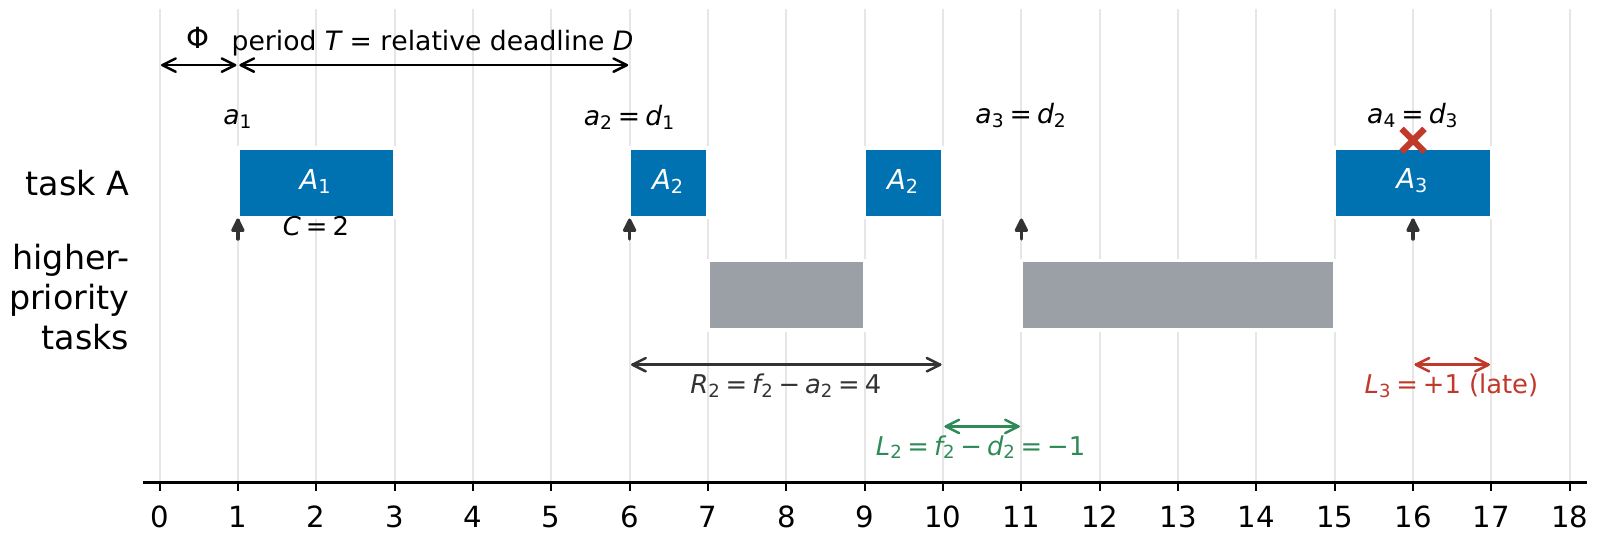
\includegraphics[width=\textwidth]{images/week-06/w6-u1-task-model.png}
    \caption{The task model on one periodic task with phase $\Phi = 1$ and $T = D = 5$: each release $a_k$ is the deadline $d_{k-1}$ of the previous job, and every job needs $C = 2$ units. Job 2 is delayed by higher-priority work: $R_2 = f_2 - a_2 = 4$, and it ends one unit before its deadline ($L_2 = -1$); job 3 ends one unit late ($L_3 = +1$).}
\end{figure}

\subsection{Fixed priorities for periodic tasks}
Every task now also needs a \textbf{priority}: \textbf{fixed} (static: chosen once, before the system starts) or \textbf{dynamic} (recomputed at run time). Fixed priorities are the easier case: the priority is one more parameter of the task, set at creation and never changed. Which task should get the higher one?

\paragraph{Example: the longer task first.} Two tasks, phase 0, $D = T$: A ($C = 2, T = 5$) and B ($C = 4, T = 10$).
\[
U = \frac{2}{5} + \frac{4}{10} = \frac{4}{10} + \frac{4}{10} = \frac{8}{10} = 0.800 \le 1
\]
The set can \emph{potentially} be scheduled, depending on the algorithm. Give the higher priority to the \textbf{longest} task: B (4 units) $>$ A (2 units). Over $H = \mathrm{LCM}(5, 10) = 10$:
\begin{verbatim}
    time  0         10
        |.........|
    A     ....####..   <- A1 misses its deadline at 5
    B     ####......
    CPU   BBBBAAAA..
\end{verbatim}
$A_1$ starts at 4 and finishes at 6, after its deadline 5: $R_{A_1} = 6 - 0 = 6 > 5$, $L_{A_1} = 6 - 5 = 1$. A late job keeps running until it completes, so $A_2$ (released at 5) runs 6--8. Answer: \texttt{schedule=BBBBAAAA..}, \texttt{feasible=no}, \texttt{first\_miss=A@5}: a deadline is \textbf{missed} although $U = 0.800$ leaves the CPU idle 20\% of the time. B could have waited until 10: with A $>$ B the set is schedulable. A is both the shorter task and the one with the shorter period; the general rule (next subsection) is that the \textbf{shorter period} means the tighter deadline, so that task goes first.

\subsection{Rate monotonic (RM)}
With fixed priorities, the problem is the assignment that makes the best use of the CPU: the highest utilisation that still meets every deadline. \textbf{Rate monotonic} (RM), found in practically every embedded system, derives a fixed priority from the \textbf{period}:
\[
\text{priority} = \frac{1}{T}
\]
The rate $1/T$ is how often a task runs: a short period gives a high priority.
\begin{itemize}
    \item \textbf{Why}: a short period means frequent releases and a deadline ($D = T$) that is always close, so the task must not wait; a long period means a far deadline and room for a small delay.
    \item \textbf{Fixed}: computed from $T$ before the system runs. Only the \textbf{order} matters, not the values $1/T$.
    \item \textbf{Preemptive}: a released job with a shorter period preempts the running one.
    \item \textbf{Same period}: the lower identifier has the higher priority (course rule); other ties as in week 5.
\end{itemize}

\paragraph{Example: the same two tasks with RM.} A ($C = 2, T = 5$) has priority $1/5$, B ($C = 4, T = 10$) has $1/10$: A $>$ B. A runs 0--2, then B; at 5, after 3 units of B, $A_2$ is released and \textbf{preempts} B (5--7); B runs its last unit 7--8.
\begin{verbatim}
    time  0         10
        |.........|
    A     ##...##...
    B     ..###..#..
    CPU   AABBBAAB..
\end{verbatim}
$A_1$ ends at $2 \le 5$, $A_2$ at $7 \le 10$, $B_1$ at $8 \le 10$ (A runs twice in one period of B): \texttt{schedule=AABBBAAB..}, \texttt{feasible=yes}, \texttt{first\_miss=none}.
\begin{figure}[H]
    \centering
    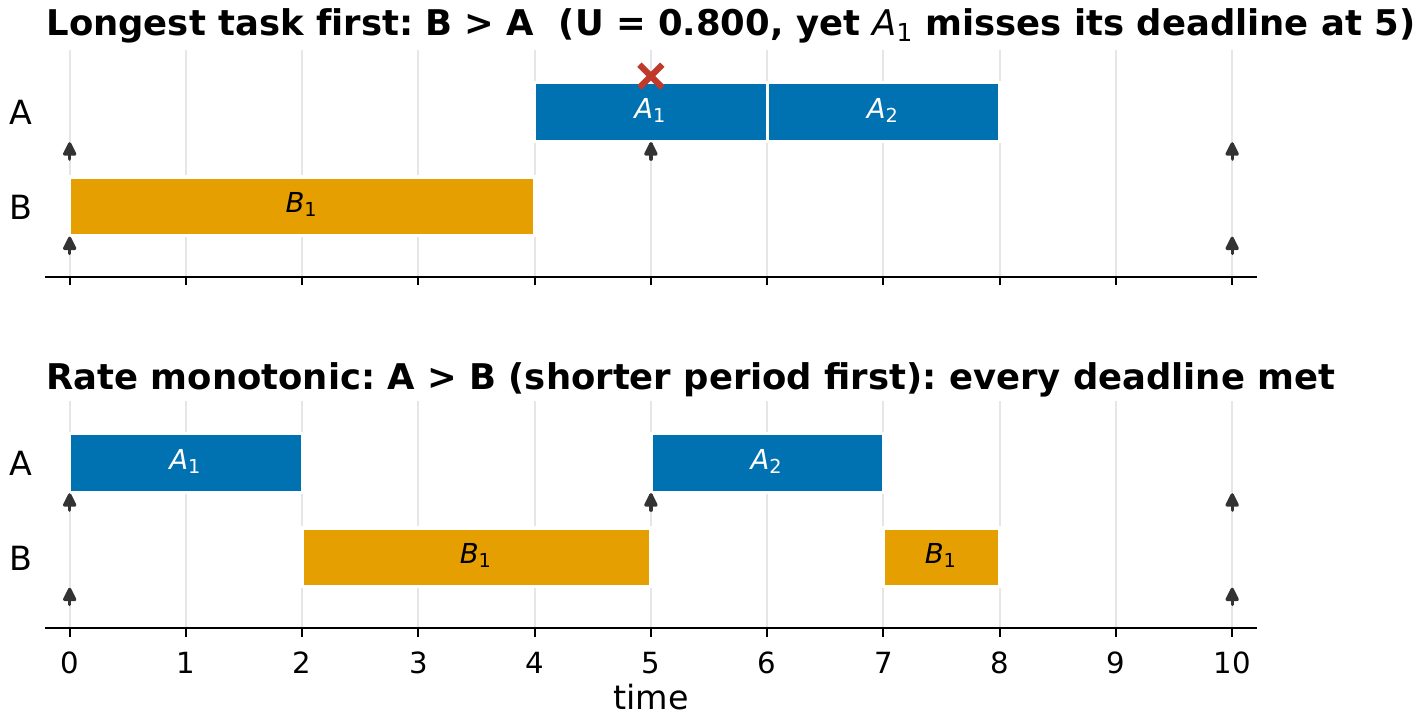
\includegraphics[width=\textwidth]{images/week-06/w6-u1-longest-vs-rm.png}
    \caption{The two priority assignments for A ($C = 2, T = 5$) and B ($C = 4, T = 10$); arrows mark the releases. With the longest task first, $A_1$ misses its deadline at 5. With rate monotonic, $A_2$ preempts B at 5 and every deadline is met.}
\end{figure}

\paragraph{Implementation.} The kernel keeps \textbf{one ready queue per priority} and runs the head of the highest non-empty one; with fixed priorities a task never changes queue.
\begin{figure}[H]
    \centering
    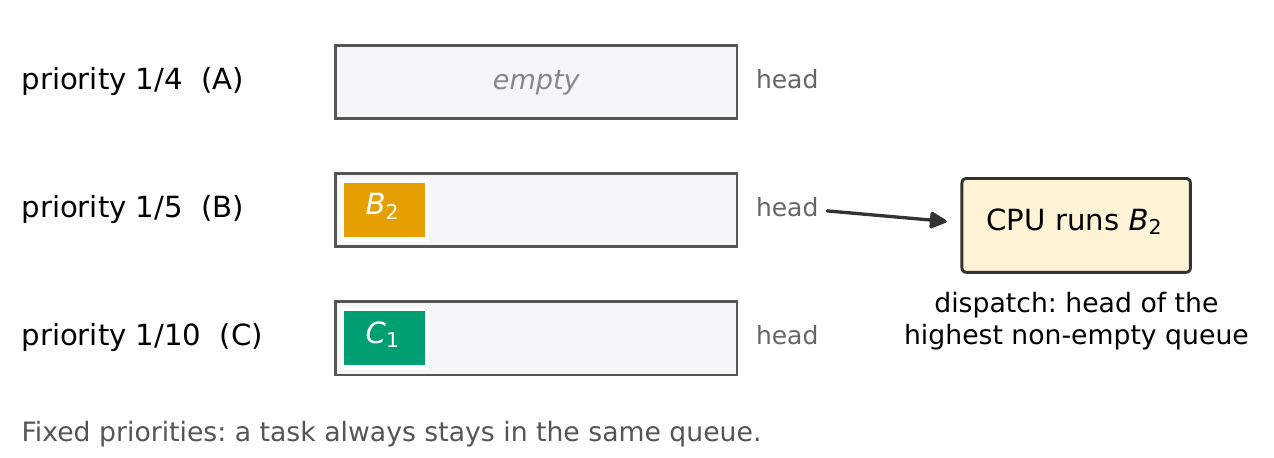
\includegraphics[width=0.8\textwidth]{images/week-06/w6-u1-rm-queues.png}
    \caption{RM implementation: one ready queue per priority. The scheduler runs the head of the highest-priority non-empty queue: here the queue of A is empty, so $B_2$ runs.}
\end{figure}

\paragraph{Tasks with the same priority.} A pure priority scheduler needs a second policy among equal priorities, any of week 5 (first-come first-served, round robin, shortest job first, \dots). FreeRTOS offers the first two: round robin if enabled, first-come first-served otherwise. In the exercises the course rule decides.

\paragraph{Where the numbers come from.} The period is a \textbf{design decision}, dictated by the safety of the users: a video player at 60 frames per second has a period of $1/60$\,s; if a car brake must react within 1\,ms, its task has a period of 1\,ms. The \textbf{WCET} must instead be \textbf{measured} (week 5), which is harder.

\subsection{RM: worked example}
Three periodic tasks: A ($C = 1, T = 4$), B ($C = 1, T = 5$), C ($C = 2, T = 10$). The period alone gives the priorities: A $>$ B $>$ C.

\paragraph{How long to draw.} With no other information, one hyperperiod, after which the schedule repeats:
\[
H = \mathrm{LCM}(4, 5, 10) = 20
\]
If every deadline in these 20 units is met, the set is feasible. A large $H$ makes drawing by hand long: the schedulability tests below give a better way to decide.

\paragraph{A method to draw by hand.} Only two \textbf{events} trigger the scheduler: the \textbf{start of a period} (a release: the task becomes ready) and the \textbf{end of a job} (another task must be chosen). Stop at every event and run the highest-priority ready task; between two events nothing changes.

\paragraph{The first steps.} No phase is given: all three tasks are released at 0.
\begin{itemize}
    \item $t = 0$: all three are ready; A, the highest priority, runs its 1 unit. At 1, $A_1$ is done (A is ready again at 4) and B runs; at 2, $B_1$ is done (B again at 5) and C runs its 2 units.
    \item $t = 4$: $C_1$ completes (C again at 10); $A_2$ is released and runs, then $B_2$ at 5.
    \item $t = 6$: nothing is ready (A returns at 8, B and C at 10): the CPU is \textbf{idle}. $A_3$ runs 8--9, then the CPU is idle until 10.
    \item $t = 10$: B and C are released: $B_3$ runs (higher priority), then $C_2$ at 11.
    \item $t = 12$: $A_4$ is released while $C_2$ runs. A has the higher priority, so C is stopped: a \textbf{preemption}. At 13 C resumes its last unit and finishes at 14 (deadline 20).
    \item Then $B_4$ (released at 15) runs at 15, and $A_5$ (released at 16) at 16.
\end{itemize}
\begin{verbatim}
    time  0         10        20
        |.........|.........|
    A     #...#...#...#...#...
    B     .#...#....#....#....
    C     ..##.......#.#......
    CPU   ABCCAB..A.BCAC.BA...
\end{verbatim}
\texttt{schedule=ABCCAB..A.BCAC.BA...}. First jobs: $R_A = 1$, $R_B = 2$, $R_C = 4$. Every job meets its deadline: \textbf{feasible}.
\begin{figure}[H]
    \centering
    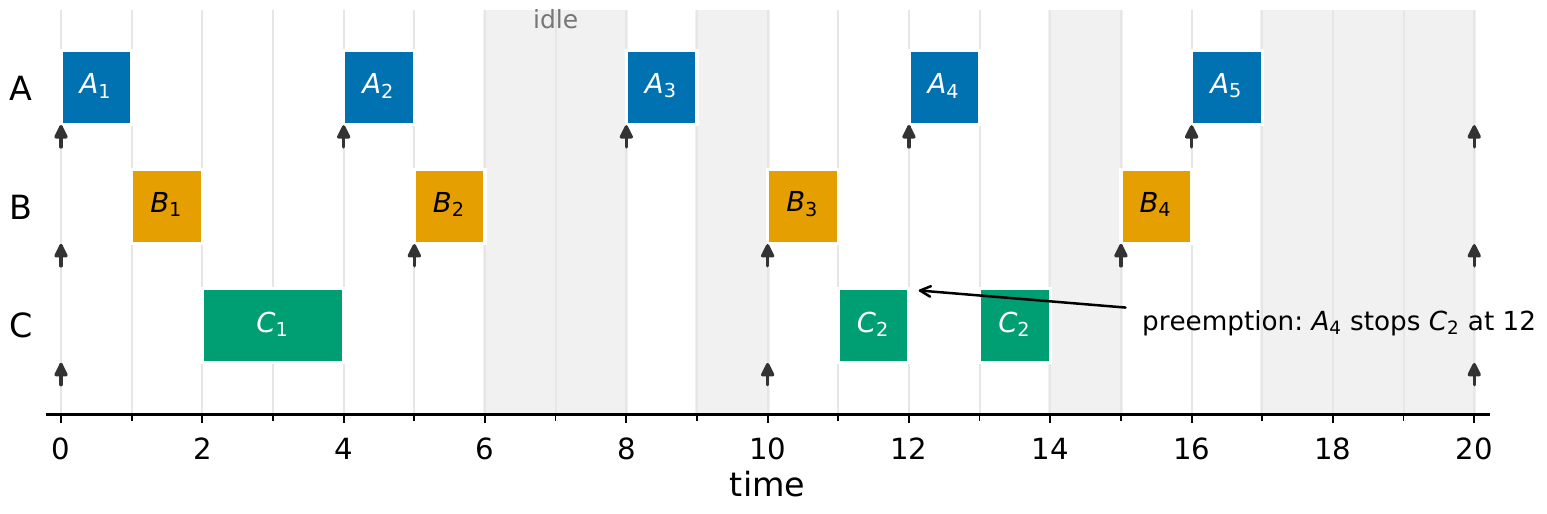
\includegraphics[width=\textwidth]{images/week-06/w6-u1-rm-example.png}
    \caption{The RM worked example over one hyperperiod ($H = 20$). Arrows mark the releases (with $D = T$, each deadline is the next release); grey bands are idle time. At 12, $A_4$ preempts $C_2$.}
\end{figure}

\subsection{Exercise: an RM schedule}
Three periodic tasks, phase 0, $D = T$, scheduled with RM: A ($C = 2, T = 5$), B ($C = 2, T = 10$), C ($C = 4, T = 20$).
\begin{enumerate}
    \item Give the priority order and compute $U$.
    \item Draw the schedule over one hyperperiod and write the schedule string.
    \item Find the response time of the \textbf{first} job of each task ($R = f - a$).
    \item Is the set feasible with RM?
\end{enumerate}
Whatever the questions, follow the exam method described at the end of the chapter: $U$ first (if $U > 1$, stop), then the priorities, then one hyperperiod from event to event.

\paragraph{Tip: mark the releases.} On paper, draw an up arrow in each task's row at the start of every period (A at 5, 10, 15 and 20; B at 10 and 20; C only at 20): you see at once when a task is ready again. The slides omit these marks.

\textbf{Solution.}
\begin{enumerate}
    \item A ($T = 5$) $>$ B ($T = 10$) $>$ C ($T = 20$).
    \[
    U = \frac{2}{5} + \frac{2}{10} + \frac{4}{20} = \frac{8}{20} + \frac{4}{20} + \frac{4}{20} = \frac{16}{20} = 0.800 \le 1
    \]
    \item $H = \mathrm{LCM}(5, 10, 20) = 20$. A runs 0--2 and B 2--4; C starts at 4, is preempted by $A_2$ at 5 (5--7), and runs its last 3 units 7--10, before A and B are released again at 10. Then $A_3$ (10--12), $B_2$ (12--14) and $A_4$ (15--17).
\begin{verbatim}
    time  0         10        20
        |.........|.........|
    A     ##...##...##...##...
    B     ..##........##......
    C     ....#..###..........
    CPU   AABBCAACCCAABB.AA...
\end{verbatim}
    \texttt{schedule=AABBCAACCCAABB.AA...}: four jobs of A, two of B and one of C per hyperperiod; from 20 the schedule repeats.
    \item $A_1$: $f = 2$, $R = 2$; \quad $B_1$: $f = 4$, $R = 4$; \quad $C_1$: $f = 10$, $R = 10$ ($C_1$ is preempted by $A_2$ at 5).
    \item Every job finishes by its deadline: feasible. The set comes back in the RTA exercise.
\end{enumerate}

\section{Schedulability tests for RM}

\subsection{Sufficient, necessary and exact tests}
$U \le 1$ is \textbf{not conclusive}: $U > 1$ means the set cannot be scheduled, but some sets with $U \le 1$ still miss a deadline. Drawing the schedule over $H$ (all phases 0) is an exact test, but:
\begin{itemize}
    \item $H$ can be very long: periods 7, 11 and 13 give $H = \mathrm{LCM}(7, 11, 13) = 1001$ slots, too many to draw by hand;
    \item real periods are in µs or ms: 20\,ms and 25\,ms at 1\,ms resolution give $H = 100$ slots for only two tasks;
    \item a designer wants a quick answer when a task is added or a WCET changes.
\end{itemize}
We want a \textbf{test}: an equation on $C$ and $T$ that decides schedulability without drawing the Gantt chart. A test is
\begin{itemize}
    \item \textbf{sufficient} if passing proves feasibility; when it fails, we know \textbf{nothing};
    \item \textbf{necessary} if failing proves infeasibility. $U \le 1$ is necessary, and \textbf{agnostic}: it holds for every algorithm;
    \item \textbf{necessary and sufficient} (``exact'') if it always answers yes or no.
\end{itemize}
Next: a test specific to RM, more precise than $U \le 1$ (Liu--Layland), then the exact test (response-time analysis).
\begin{figure}[H]
    \centering
    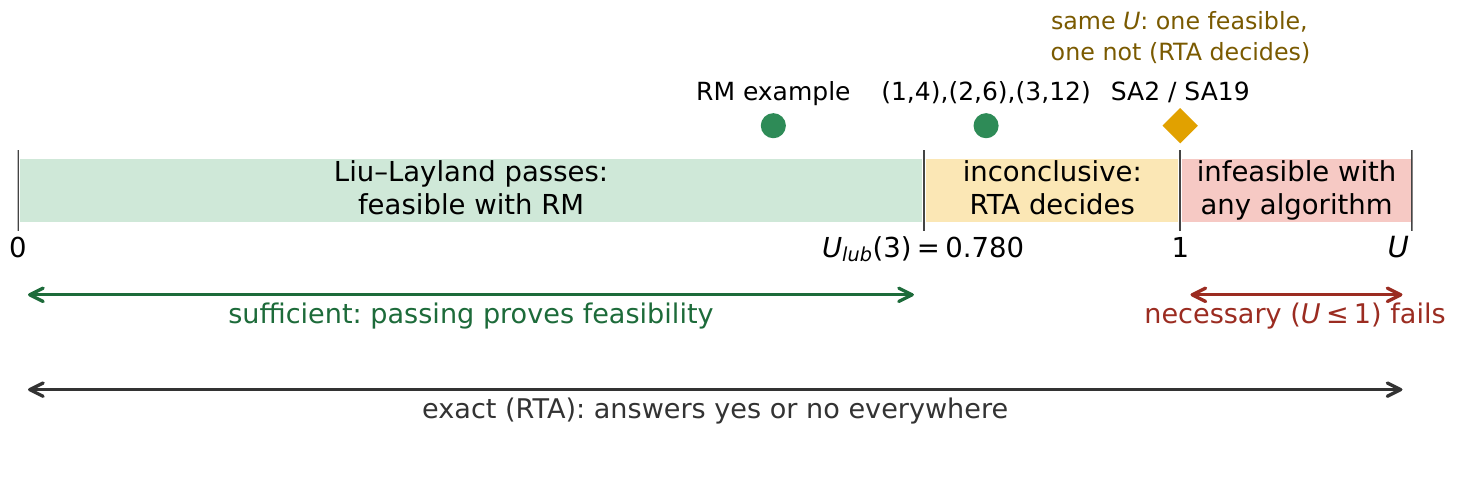
\includegraphics[width=\textwidth]{images/week-06/w6-u1-tests.png}
    \caption{The three kinds of test on the utilisation axis, for $n = 3$ tasks. Liu--Layland is sufficient: below 0.780 it proves feasibility. $U \le 1$ is necessary: above 1 no algorithm works. In between only an exact test decides: SA2 and SA19 both have $U = 1$, and RTA shows that only SA2 is feasible with RM.}
\end{figure}

\subsection{The Liu--Layland bound}
Liu and Layland (1973) showed that for RM the threshold is not 1: $n$ periodic tasks (our model, $D = T$) are feasible with RM if
\[
U = \sum_{i=1}^{n} \frac{C_i}{T_i} \le U_{lub}(n) = n \left( 2^{1/n} - 1 \right)
\]
$U_{lub}$ is the \textbf{least upper bound}: up to it, RM meets every deadline, for any periods. It depends only on the number of tasks $n$:
\begin{center}
    \begin{tabular}{c | c c c c c c c}
        \hline
        $n$ & 1 & 2 & 3 & 4 & 5 & 10 & $n \to \infty$ \\
        \hline
        $U_{lub}(n)$ & 1.000 & 0.828 & 0.780 & 0.757 & 0.743 & 0.718 & $\ln 2 \approx 0.693$ \\
        \hline
    \end{tabular}
\end{center}

\paragraph{How to use it.} Compare $U$, with three decimals, with $U_{lub}(n)$ for the $n$ of the set instead of with 1. Remember the equation, not the table: with three tasks, put $n = 3$: $3 \times (2^{1/3} - 1) = 0.780$.
\begin{itemize}
    \item $U \le U_{lub}(n)$: \textbf{feasible with RM}, done. Examples: the first two-task set ($U = 0.800 \le 0.828$) and the RM worked example ($U = 1/4 + 1/5 + 2/10 = 0.650 \le 0.780$).
    \item $U_{lub}(n) < U \le 1$: \textbf{inconclusive}: the set may or may not be feasible.
    \item $U > 1$: not feasible, with RM or any other algorithm.
    \item The bound is \textbf{sufficient, not necessary}: a set above it can still be feasible.
\end{itemize}

\paragraph{The bound as a function of $n$.} $U_{lub}(n)$ decreases from 1 at $n = 1$. Above the line $U = 1$ every set is infeasible; below the curve RM is guaranteed; in between, a more precise test is needed. As $n \to \infty$:
\[
\lim_{n \to \infty} n \left( 2^{1/n} - 1 \right) = \ln 2 \approx 0.693
\]
so a set with $U \le 0.693$ is always feasible with RM, whatever $n$.
\begin{figure}[H]
    \centering
    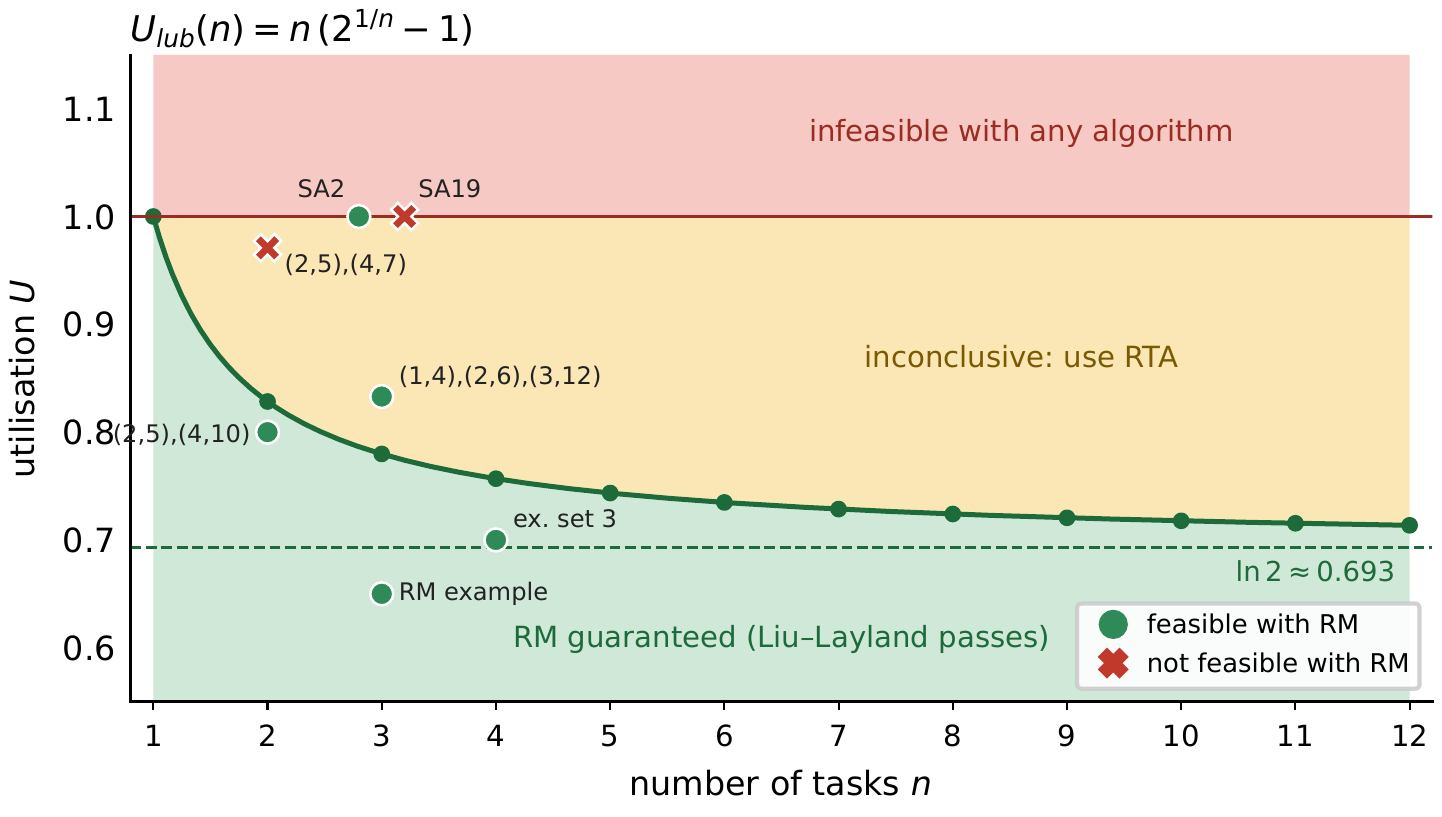
\includegraphics[width=0.92\textwidth]{images/week-06/w6-u1-liu-layland.png}
    \caption{The Liu--Layland bound $U_{lub}(n)$, decreasing towards $\ln 2$, with the task sets of these notes. Below the curve RM is guaranteed; between the curve and $U = 1$ both outcomes occur, and RTA decides; above 1 no algorithm can meet every deadline.}
\end{figure}

\subsection{Above the bound: two sets, two outcomes}
Above the bound the test is inconclusive and both outcomes are possible. Sets written as ($C$, $T$):

\paragraph{A (1, 4), B (2, 6), C (3, 12): feasible.}
\[
U = \frac{1}{4} + \frac{2}{6} + \frac{3}{12} = \frac{3}{12} + \frac{4}{12} + \frac{3}{12} = \frac{10}{12} = \frac{5}{6} = 0.833 > 0.780
\]
\begin{verbatim}
    time  0         10
        |.........|..
    A     #...#...#...
    B     .##...##....
    C     ...#.#...#..
    CPU   ABBCACBBAC..
\end{verbatim}
$H = \mathrm{LCM}(4, 6, 12) = 12$: every deadline is met.

\paragraph{A (2, 5), B (4, 7): not feasible.}
\[
U = \frac{2}{5} + \frac{4}{7} = \frac{14}{35} + \frac{20}{35} = \frac{34}{35} = 0.971 > 0.828
\]
\begin{verbatim}
    time  0         10        20        30
        |.........|.........|.........|....
    A     ##...##...##...##...##...##...##...
    B     ..###..###..###..###..###..###..##.   <- B1 misses its deadline at 7
    CPU   AABBBAABBBAABBBAABBBAABBBAABBBAABB.
\end{verbatim}
$H = \mathrm{LCM}(5, 7) = 35$. $B_1$ runs 2--5, is preempted by $A_2$ at 5, and finishes at 8, after its deadline 7: \texttt{first\_miss=B@7}.

Same verdict of the test, opposite answers: deciding needs an \textbf{exact} test for RM.

\subsection{Exercise: the bound test}
Four task sets, phase 0, $D = T$, RM, written as ($C$, $T$):
\begin{enumerate}
    \item A (1, 4), B (2, 8)
    \item A (1, 2), B (1, 3)
    \item A (1, 4), B (1, 5), C (2, 10), D (1, 20)
    \item A (3, 5), B (3, 6)
\end{enumerate}
For each set compute $U$ and $U_{lub}(n)$ with three decimals and give the verdict of the Liu--Layland test: feasible with RM, inconclusive, or not feasible at all. For set 2, draw the RM schedule over $H = 6$ to decide.

\textbf{Solution.}
\begin{center}
    \begin{tabular}{c l c c l}
        \hline
        set & $U$ & $U_{lub}(n)$ & compare & verdict \\
        \hline
        1 & $1/4 + 2/8 = 0.500$ & $U_{lub}(2) = 0.828$ & $0.500 \le 0.828$ & feasible with RM \\
        2 & $1/2 + 1/3 = 5/6 = 0.833$ & $U_{lub}(2) = 0.828$ & $0.833 > 0.828$ & inconclusive \\
        3 & $1/4 + 1/5 + 2/10 + 1/20 = 14/20 = 0.700$ & $U_{lub}(4) = 0.757$ & $0.700 \le 0.757$ & feasible with RM \\
        4 & $3/5 + 3/6 = 11/10 = 1.100$ & & $U > 1$ & not feasible (any algorithm) \\
        \hline
    \end{tabular}
\end{center}
Set 2 with RM:
\begin{verbatim}
    time  0     6
        |.....|
    A     #.#.#.
    B     .#.#..
    CPU   ABABA.
\end{verbatim}
\texttt{schedule=ABABA.}: $B_1$ finishes at $2 \le 3$, $B_2$ at $4 \le 6$: set 2 is feasible, although above the bound. Set 3 is the RM worked example plus D: one more task lowers the bound from 0.780 to 0.757.

\subsection{Response-time analysis (RTA)}
The exact test for RM is not a formula but an \textbf{algorithm}, based on the \textbf{response time} of each task.

\paragraph{The foundation.} A ready task can be delayed only by tasks with a higher priority that run: their execution time is the \textbf{interference} on it. RTA bounds the \textbf{maximum delay} they can cause, computing $R$ in windows of time from their execution times and periods.

\paragraph{Which tasks count.} Number five tasks from 1 (lowest priority) to 5 (highest): the $R$ of task 1 depends on tasks 2, 3, 4 and 5, that of task 2 on tasks 3, 4 and 5, and so on. Task 5 has no task above it: no interference, it always runs at the start of its period, so $R = C$.

\paragraph{Why the release at 0 is the worst case.} RTA needs the \textbf{worst} response time of the jobs of each task. The interference on a job is largest when every higher-priority task releases a job \textbf{at the same instant}: the \textbf{critical instant} (Liu and Layland). With all phases 0, every task releases its first job at 0, so \textbf{the first job of each task has the worst response time}, and $R_i$ is its finish time.

\paragraph{The equation.} $R_i$ is the task's own time plus the interference. In a window of length $R$, a higher-priority task $j$ releases $\lceil R / T_j \rceil$ jobs ($\lceil x \rceil$ = round \textbf{up}, e.g.\ $\lceil 7/4 \rceil = 2$), each taking $C_j$:
\[
R_i = C_i + \sum_{j \in hp(i)} \left\lceil \frac{R_i}{T_j} \right\rceil C_j
\]
where $hp(i)$ is the set of tasks with a higher priority than $i$. $R_i$ is on both sides, so the equation is solved by \textbf{iteration}:
\begin{itemize}
    \item \textbf{start}: no interference yet, $R_i^{(0)} = C_i$;
    \item \textbf{step}: $R_i^{(k+1)} = C_i + \sum_{j \in hp(i)} \lceil R_i^{(k)} / T_j \rceil \, C_j$, the interference of the higher-priority jobs released in $[0, R_i^{(k)})$;
    \item \textbf{stop 1}, a \textbf{fixed point}: $R_i^{(k+1)} = R_i^{(k)}$. The value cannot change any more: $R_i = R_i^{(k)}$ is the window in which the task, released at the start of its period, completes. If $R_i \le D_i$, task $i$ meets its deadline;
    \item \textbf{stop 2}: $R_i^{(k+1)} > D_i$: the deadline is missed, there is no need to go on, and $R_i$ is that first value above $D_i$ (course rule).
\end{itemize}
For the highest-priority task the sum is empty, and $R = C$ is already a fixed point. The set is feasible with RM \textbf{if and only if} $R_i \le D_i$ for every task: RTA is exact (for our model), and one task that misses proves the set unschedulable.

\subsection{RTA: worked example}
The feasible set above the bound: A ($C = 1, T = 4$), B ($C = 2, T = 6$), C ($C = 3, T = 12$), $D = T$, RM: A $>$ B $>$ C. $U = 0.833 > U_{lub}(3) = 0.780$: inconclusive, so we use RTA.

\paragraph{Task A.} Highest priority: $R_A = C_A = 1$, and $1 \le 4$: \textbf{met}.

\paragraph{Task B.} Higher priority: only A.
\[
\begin{aligned}
R_B^{(0)} &= C_B = 2 \\
R_B^{(1)} &= 2 + \left\lceil \tfrac{2}{4} \right\rceil \cdot 1 = 2 + 1 = 3 \\
R_B^{(2)} &= 2 + \left\lceil \tfrac{3}{4} \right\rceil \cdot 1 = 2 + 1 = 3
\end{aligned}
\]
$2/4 = 0.5$ rounds up to 1: one job of A falls in the window. $R_B^{(1)} = 3$ differs from the previous value, so we iterate; $R_B^{(2)} = R_B^{(1)}$: fixed point, $R_B = 3 \le 6$: met.

\paragraph{Task C.} Higher priority: A and B, so the sum has two terms.
\[
\begin{aligned}
R_C^{(0)} &= C_C = 3 \\
R_C^{(1)} &= 3 + \left\lceil \tfrac{3}{4} \right\rceil \cdot 1 + \left\lceil \tfrac{3}{6} \right\rceil \cdot 2 = 3 + 1 + 2 = 6 \\
R_C^{(2)} &= 3 + \left\lceil \tfrac{6}{4} \right\rceil \cdot 1 + \left\lceil \tfrac{6}{6} \right\rceil \cdot 2 = 3 + 2 + 2 = 7 \\
R_C^{(3)} &= 3 + \left\lceil \tfrac{7}{4} \right\rceil \cdot 1 + \left\lceil \tfrac{7}{6} \right\rceil \cdot 2 = 3 + 2 + 4 = 9 \\
R_C^{(4)} &= 3 + \left\lceil \tfrac{9}{4} \right\rceil \cdot 1 + \left\lceil \tfrac{9}{6} \right\rceil \cdot 2 = 3 + 3 + 4 = 10 \\
R_C^{(5)} &= 3 + \left\lceil \tfrac{10}{4} \right\rceil \cdot 1 + \left\lceil \tfrac{10}{6} \right\rceil \cdot 2 = 3 + 3 + 4 = 10
\end{aligned}
\]
$R_C^{(5)} = R_C^{(4)}$: fixed point, $R_C = 10 \le 12$: met. Each step adds the jobs released before the previous $R$: $A_2$ (released at 4) enters at 6, $B_2$ (at 6) at 7, $A_3$ (at 8) at 9; at 10 nothing new enters.

\paragraph{Result.} Every $R \le D$: feasible with RM, although $U = 0.833 > 0.780$. The Gantt chart drawn earlier for this set agrees: $A_1$ ends at 1, $B_1$ at 3, $C_1$ at 10. Being exact, RTA spares a designer the Gantt chart: the system works, as long as the WCETs used are the true ones.
\begin{figure}[H]
    \centering
    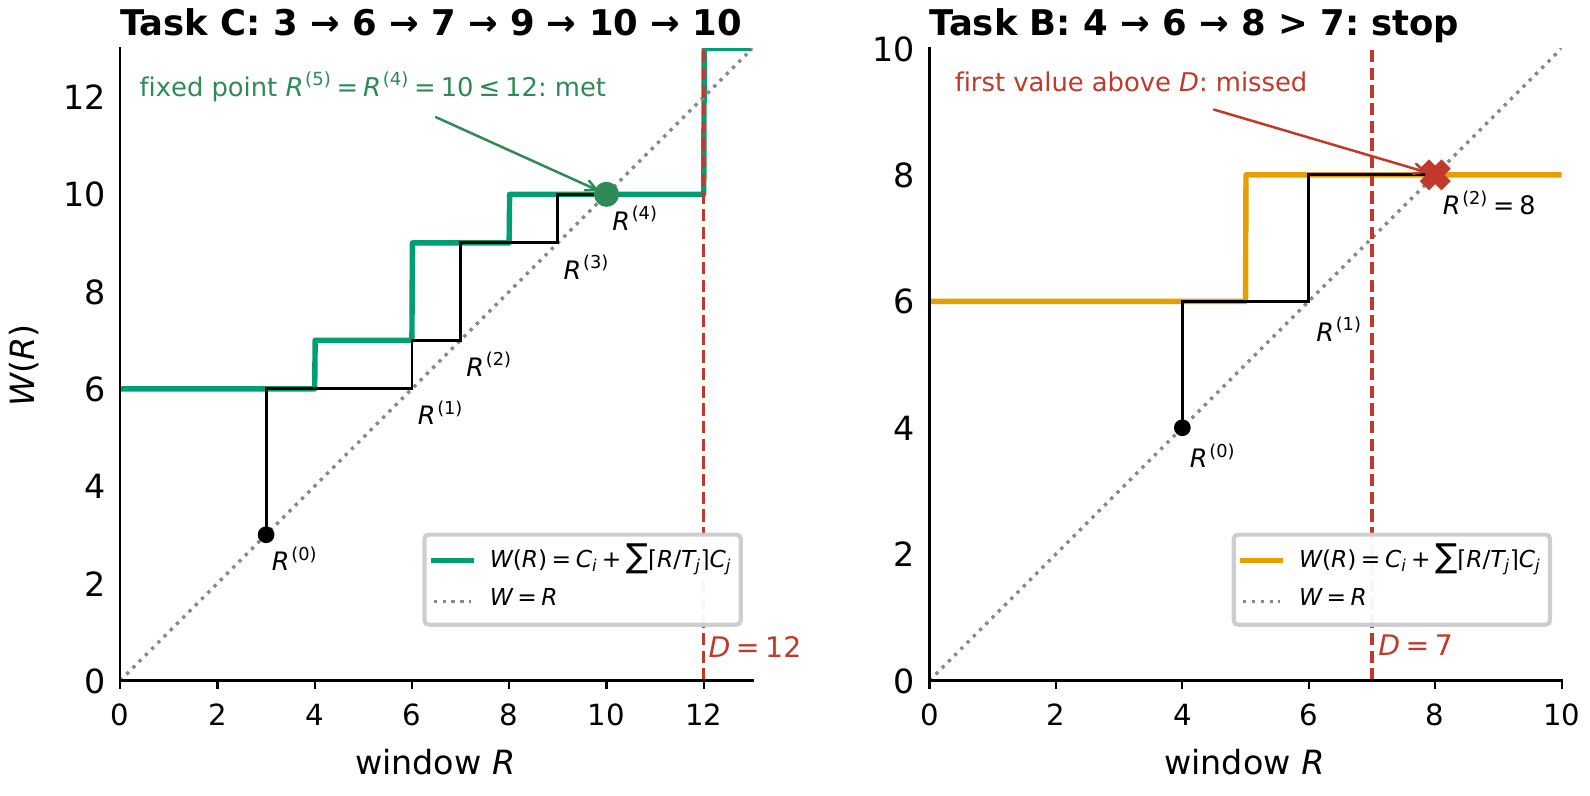
\includegraphics[width=\textwidth]{images/week-06/w6-u1-rta-iteration.png}
    \caption{RTA as a fixed-point iteration. The step function $W(R) = C_i + \sum_j \lceil R/T_j \rceil C_j$ is the work released in a window of length $R$; each iterate is read on the curve and brought back to the diagonal $W = R$. Left: task C of the worked example reaches the fixed point $R_C = 10 \le 12$. Right: task B of the set A ($C = 2, T = 5$), B ($C = 4, T = 7$) jumps to 8, above $D = 7$, and the iteration stops.}
\end{figure}

\paragraph{Three tests for fixed priorities.} $U \le 1$, necessary for every algorithm; $U \le U_{lub}(n)$ (Liu--Layland), specific to RM and sufficient only; RTA, an algorithm that is exact.

\subsection{RTA when a deadline is missed}
A ($C = 2, T = 5$), B ($C = 4, T = 7$), RM: $U = 0.971 > 0.828$, inconclusive.

\paragraph{Task A.} Highest priority: $R_A = C_A = 2 \le 5$: met.

\paragraph{Task B.} Higher priority: only A.
\[
\begin{aligned}
R_B^{(0)} &= C_B = 4 \\
R_B^{(1)} &= 4 + \left\lceil \tfrac{4}{5} \right\rceil \cdot 2 = 4 + 2 = 6 \\
R_B^{(2)} &= 4 + \left\lceil \tfrac{6}{5} \right\rceil \cdot 2 = 4 + 4 = 8
\end{aligned}
\]
$R_B^{(2)} = 8$ is not a fixed point, but it is already above the deadline $D_B = 7$: stop, $R_B = 8$, deadline missed: the set cannot be scheduled with RM. The window $[0, 6)$ contains $A_2$ (released at 5): 2 more units of interference. The Gantt chart drawn earlier for this set confirms it: $B_1$ finishes at 8, one unit after its deadline; the first miss is \texttt{B@7}.

\subsection{Try it: explain an RM set with schedsim}
\texttt{schedsim}, used last week for the timeline, can also \texttt{explain}, \texttt{solve} and \texttt{check} RM exercises, printing the bound test and every RTA iteration. The task-set file of the RTA example is \texttt{images/week-06/w6-u1-rm-rta.txt}:
\begin{lstlisting}
    algorithm: rm
    task A C=1 T=4
    task B C=2 T=6
    task C C=3 T=12
\end{lstlisting}
From the folder that contains your copy of \texttt{course-material}:
\begin{lstlisting}[language=bash]
    cd course-material/tools/schedsim
    python3 schedsim.py explain ../../images/week-06/w6-u1-rm-rta.txt
\end{lstlisting}
Output (excerpt):
\begin{verbatim}
    == Utilization test (Liu-Layland) ==
    U = sum C/T = 1/4 + 2/6 + 3/12 = 5/6 = 0.833
    bound = n(2^(1/n) - 1) = 3*(2^(1/3) - 1) = 0.780
    0.833 vs 0.780  ->  U > bound: test inconclusive, use RTA

    == Response-time analysis (RTA) ==
    Priority order (shorter period = higher priority): A > B > C
    R(0) = C;  R(k+1) = C + sum over higher priority j of ceil(R(k)/Tj)*Cj;
    stop at a fixed point or when R > D.
    ...
    C (C=3, D=12), higher priority: A, B
      R(0) = C_C = 3
      R(1) = 3 + ceil(3/4)*1 + ceil(3/6)*2 = 6
      R(2) = 3 + ceil(6/4)*1 + ceil(6/6)*2 = 7
      R(3) = 3 + ceil(7/4)*1 + ceil(7/6)*2 = 9
      R(4) = 3 + ceil(9/4)*1 + ceil(9/6)*2 = 10
      R(5) = 3 + ceil(10/4)*1 + ceil(10/6)*2 = 10
      R(5) = R(4): fixed point, R_C = 10
      R_C = 10 <= D = 12: deadline met
\end{verbatim}
The output continues with A and B, the chart \texttt{ABBCACBBAC..}, the job table and every decision: compare the iterations of C with the worked example.

\paragraph{Exam.} The exam requires the algorithms and the schedulability conditions, RTA included; the details are at the end of the chapter.

\subsection{Exercise: RTA}
The set of the RM exercise, with RM: A ($C = 2, T = 5$), B ($C = 2, T = 10$), C ($C = 4, T = 20$).
\begin{enumerate}
    \item Compute $U_{lub}(3)$ and apply the Liu--Layland test ($U = 0.800$). What does it tell you?
    \item Compute $R_A$, $R_B$ and $R_C$ with RTA. Write every iteration.
    \item Is the set feasible with RM? Compare each $R$ with the first-job response times you found in the schedule.
\end{enumerate}

\textbf{Solution.}
\begin{enumerate}
    \item $U_{lub}(3) = 3 \times (2^{1/3} - 1) = 0.780$; $0.800 > 0.780$: inconclusive, use RTA.
    \item A: no higher priority, $R_A = C_A = 2 \le 5$: met.

    B: higher A.
    \[
    R_B^{(0)} = 2, \quad R_B^{(1)} = 2 + \left\lceil \tfrac{2}{5} \right\rceil \cdot 2 = 4, \quad R_B^{(2)} = 2 + \left\lceil \tfrac{4}{5} \right\rceil \cdot 2 = 4
    \]
    Fixed point, $R_B = 4 \le 10$: met.

    C: higher A and B.
    \[
    \begin{aligned}
    R_C^{(0)} &= 4 \\
    R_C^{(1)} &= 4 + \left\lceil \tfrac{4}{5} \right\rceil \cdot 2 + \left\lceil \tfrac{4}{10} \right\rceil \cdot 2 = 4 + 2 + 2 = 8 \\
    R_C^{(2)} &= 4 + \left\lceil \tfrac{8}{5} \right\rceil \cdot 2 + \left\lceil \tfrac{8}{10} \right\rceil \cdot 2 = 4 + 4 + 2 = 10 \\
    R_C^{(3)} &= 4 + \left\lceil \tfrac{10}{5} \right\rceil \cdot 2 + \left\lceil \tfrac{10}{10} \right\rceil \cdot 2 = 4 + 4 + 2 = 10
    \end{aligned}
    \]
    Fixed point, $R_C = 10 \le 20$: met. In $R_C^{(3)}$, $A_3$ and $B_2$ are released at 10, but the window $[0, 10)$ does not contain them: $\lceil 10/5 \rceil = 2$, not 3.
    \item \textbf{Feasible with RM}. The schedule \texttt{AABBCAACCCAABB.AA...} gave $A_1$: 2, $B_1$: 4, $C_1$: 10: the same values.
\end{enumerate}

\section{Unit 1: summary}
\begin{itemize}
    \item Fixed priorities: the shorter period goes first. \textbf{Rate monotonic}: priority $1/T$, fixed, preemptive; one ready queue per priority.
    \item Draw one hyperperiod from event to event (releases and completions), running the highest-priority ready task.
    \item \textbf{Sufficient} test: passing proves feasibility, failing says nothing. \textbf{Necessary}: failing proves infeasibility. \textbf{Exact}: always answers.
    \item \textbf{Liu--Layland}: RM is feasible if $U \le n(2^{1/n} - 1)$: 0.828 for 2 tasks, 0.780 for 3, down to $\ln 2 \approx 0.693$. Sufficient, \textbf{not necessary}: above the bound a set may still be feasible.
    \item \textbf{Critical instant}: all tasks released together gives the worst response time, that of the first job with phase 0.
    \item \textbf{RTA}: $R^{(k+1)} = C_i + \sum \lceil R^{(k)} / T_j \rceil C_j$ over the higher-priority tasks, from $R^{(0)} = C_i$ until a fixed point or $R > D$. Exact for RM.
    \item \texttt{schedsim explain} prints the bound test and every RTA iteration: use it to check paper solutions. One exam exercise is always on scheduling.
\end{itemize}

\section{Unità 2 - Dynamic priorities and one-shot jobs: EDF, Jackson, Horn}
This unit adds an algorithm with \textbf{dynamic priorities} for periodic tasks, then the second problem of real-time scheduling: not everything is periodic, and \textbf{aperiodic} jobs must be scheduled too.

\subsection{Earliest Deadline First (EDF)}
RM is not \textbf{optimal}: an optimal algorithm schedules every set that some algorithm can schedule, which with $D = T$ means every set with $U \le 1$, up to 100\% of the CPU. To get there, drop the only constraint of RM, the fixed priorities: priorities computed at run time adapt to the situation of the tasks, at the price of a more complex scheduler. The priority now comes from the \textbf{deadline} of the job.

\paragraph{The rule.} \textbf{EDF} runs, at every instant, the ready job closest to its deadline: the one with the \textbf{earliest absolute deadline} $d = a + D$.
\begin{itemize}
    \item The priority belongs to the \textbf{job}, not to the task: two jobs of the same task have different deadlines. Priorities are dynamic: the order between two tasks changes over time.
    \item \textbf{Preemptive}: a released job with a strictly earlier deadline preempts the running one.
    \item Same deadline: tie rules of week 5.
\end{itemize}

\paragraph{Where the complexity is.} Whenever the set of ready jobs changes, the scheduler must first \textbf{recompute the priorities}, and only then choose: at each release the kernel computes $d$ and keeps the ready jobs ordered by $d$.
\begin{figure}[H]
    \centering
    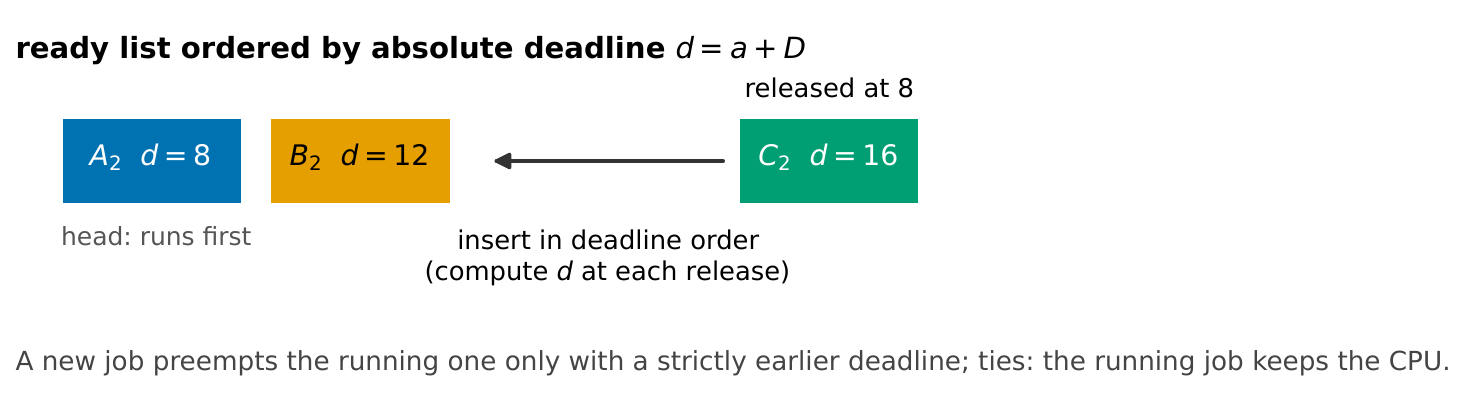
\includegraphics[width=0.85\textwidth]{images/week-06/w6-u2-edf-list.png}
    \caption{EDF bookkeeping: the ready jobs are kept ordered by absolute deadline. At each release the kernel computes $d = a + D$ and inserts the job in place; the head runs.}
\end{figure}

\subsection{The EDF test: $U \le 1$}
Liu and Layland also proved that, in our model (independent, preemptive, $D = T$, one CPU), a set of periodic tasks is feasible with EDF if and only if
\[
U = \sum_{i=1}^{n} \frac{C_i}{T_i} \le 1
\]
\begin{itemize}
    \item \textbf{Necessary and sufficient}: the general condition of week 5 is now an exact test, with no bound and no iteration: $U \le 1$, every deadline is met; $U > 1$, some deadline is missed.
    \item EDF can use \textbf{100\%} of the CPU (on the plot of $U_{lub}(n)$, everything up to the line $U = 1$); RM is guaranteed only up to $U_{lub}(n)$, never below 69\%.
    \item EDF is optimal on one CPU: if some algorithm meets every deadline of the set, EDF does too.
\end{itemize}
The Gantt chart is still drawn over one hyperperiod.

\subsection{EDF: worked example}
A ($C = 1, T = 4$), B ($C = 2, T = 6$), C ($C = 3, T = 8$).
\[
U = \frac{1}{4} + \frac{2}{6} + \frac{3}{8} = \frac{6}{24} + \frac{8}{24} + \frac{9}{24} = \frac{23}{24} = 0.958 \le 1
\]
Far above the RM bound 0.780, yet feasible with EDF. $H = \mathrm{LCM}(4, 6, 8) = 24$; at every event the priorities are recomputed from the deadlines.
\begin{itemize}
    \item $t = 0$: deadlines $A_1$: 4, $B_1$: 6, $C_1$: 8, so A $>$ B $>$ C: A runs (1 unit), then B (2 units), then C. Nothing changes the deadlines before 4.
    \item $t = 4$: $A_2$ is released with $d = 8$, the \textbf{same} deadline as the running $C_1$ ($B_2$ is not released yet): on a tie the running job keeps the CPU, so C ends at 6. With RM, $A_2$ would have preempted $C_1$.
    \item $t = 6$: $C_1$ finishes and $B_2$ is released ($d = 12$); $A_2$ ($d = 8$) is earlier and runs 1 unit, then B.
    \item $t = 8$: $A_3$ ($d = 12$) is released while $B_2$ ($d = 12$) runs: tie, B keeps the CPU. $C_2$, released with $d = 16$, waits. B ends at 9, then $A_3$ runs, then C from 10.
    \item $t = 12$: $A_4$ ($d = 16$) is released while $C_2$ ($d = 16$) runs: tie, C keeps the CPU.
    \item $t = 20$: $A_6$ ($d = 24$) and $B_4$ ($d = 24$) tie and neither is running (C just ended): lowest identifier, A.
\end{itemize}
\begin{verbatim}
    time  0         10        20
        |.........|.........|...
    A     #.....#..#...#..#...#...
    B     .##....##.....##.....##.
    C     ...###....###....###....
    CPU   ABBCCCABBACCCABBACCCABB.
\end{verbatim}
\texttt{schedule=ABBCCCABBACCCABBACCCABB.}: no deadline is missed, feasible, with $U = 0.958$.
\begin{figure}[H]
    \centering
    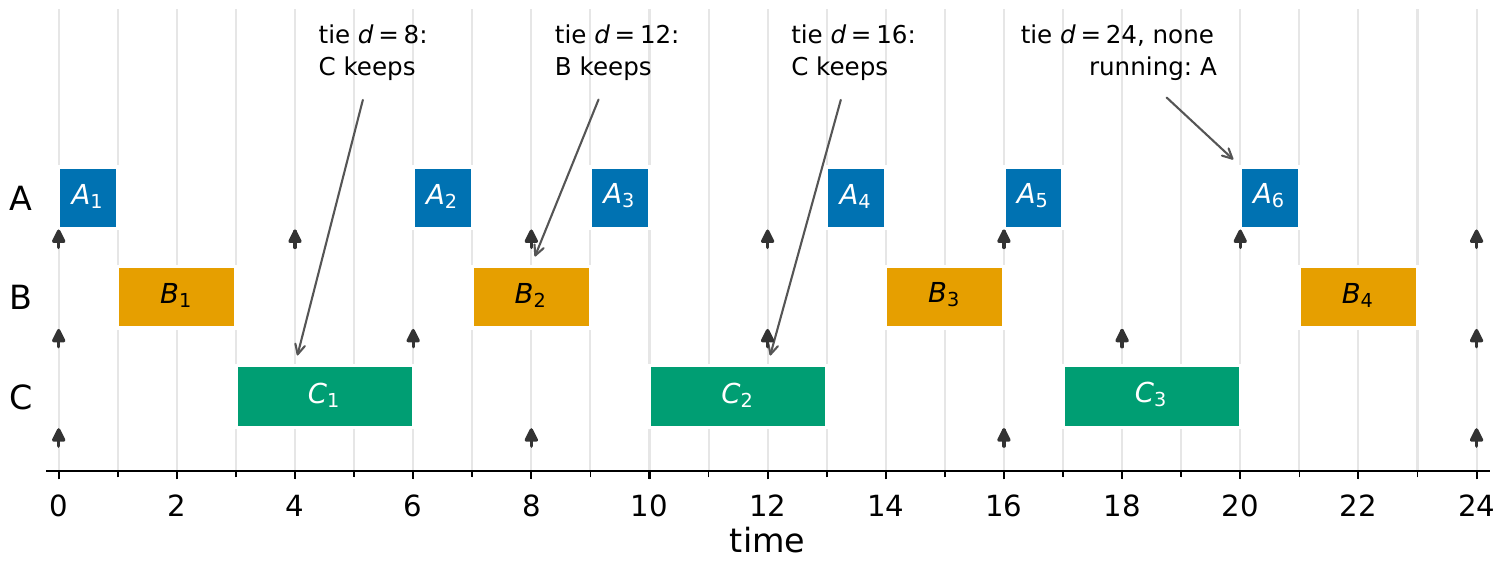
\includegraphics[width=\textwidth]{images/week-06/w6-u2-edf-example.png}
    \caption{The EDF worked example ($H = 24$). The callouts mark the ties: a job released with the same deadline as the running one does not preempt it; when neither tied job is running, the lowest identifier wins.}
\end{figure}

\paragraph{Solving EDF exercises by hand.} Use the event method of the RM worked example as an \textbf{algorithmic} procedure: \textbf{mark all the periods} (every period start is an event), then go left to right through releases and completions, recomputing the deadlines at each event. RM is the same without the recomputation. Any layout works (one line per task, or one timeline), as long as you have a method.

\subsection{Exercise: an EDF schedule}
Three periodic tasks, phase 0, $D = T$, scheduled with EDF: A ($C = 1, T = 4$), B ($C = 2, T = 5$), C ($C = 3, T = 10$).
\begin{enumerate}
    \item Compute $U$ and apply the EDF test.
    \item Draw the EDF schedule over one hyperperiod and write the schedule string. At every tie, write which rule decides.
    \item Which job is preempted, and when? Which ties occur at 5 and at 16?
    \item Give \texttt{feasible} and \texttt{first\_miss}.
\end{enumerate}

\textbf{Solution.}
\begin{enumerate}
    \item \[
    U = \frac{1}{4} + \frac{2}{5} + \frac{3}{10} = \frac{5}{20} + \frac{8}{20} + \frac{6}{20} = \frac{19}{20} = 0.950 \le 1
    \]
    Feasible with EDF.
    \item $H = \mathrm{LCM}(4, 5, 10) = 20$. At 0, A has the earliest deadline and runs. When A completes, the deadlines are evaluated again: the next deadline of A is 8, that of B is 5, that of C is 10, so B runs; and so on.
\begin{verbatim}
    time  0         10        20
        |.........|.........|
    A     #...#....#..#...#...
    B     .##..##...##.....##.
    C     ...#...##....###....
    CPU   ABBCABBCCABBACCCABB.
\end{verbatim}
    \texttt{schedule=ABBCABBCCABBACCCABB.}
    \item At 4, $A_2$ ($d = 8$) arrives while $C_1$ ($d = 10$) runs: $A_2$ preempts $C_1$. At 5, $B_2$ ($d = 10$) and $C_1$ ($d = 10$) are tied and neither is running ($A_2$ just ended): lowest identifier, B. $C_1$ runs in slot 3, waits for $A_2$ and $B_2$, and ends at $9 \le 10$. At 15, $B_4$ ($d = 20$) arrives while $C_2$ ($d = 20$) runs: C keeps the CPU. At 16, $A_5$ ($d = 20$) and $B_4$ ($d = 20$) are tied and neither is running ($C_2$ just ended): lowest identifier, A.
    \item \texttt{feasible=yes}, \texttt{first\_miss=none}.
\end{enumerate}

\subsection{RM vs EDF on the same set}
A set built to show that EDF does better than RM: A ($C = 2, T = 5$), B ($C = 4, T = 7$), $U = 34/35 = 0.971 \le 1$, $H = 35$.
\begin{itemize}
    \item \textbf{RM}: A always before B. $U > 0.828$, and RTA gives $R_B = 8 > 7$: $B_1$ misses its deadline, \texttt{first\_miss=B@7}, as its chart in Unit 1 shows.
    \item \textbf{EDF}: $U \le 1$: feasible. At 5, $A_2$ ($d = 10$) does \textbf{not} preempt $B_1$ ($d = 7$), which ends at 6.
\end{itemize}
\begin{verbatim}
    time  0         10        20        30
        |.........|.........|.........|....
    A     ##....##....##.##...##....##....##.
    B     ..####..####..#..###..####..####...
    CPU   AABBBBAABBBBAABAABBBAABBBBAABBBBAA.
\end{verbatim}
At 5, RM gives the CPU to $A_2$ because of its period; EDF lets $B_1$ finish because its deadline is closer. Over $H = 35$, EDF preempts once (at 15, where $A_4$, $d = 20$, preempts $B_3$, $d = 21$), RM five times (at 5, 10, 15, 25 and 30).
\begin{figure}[H]
    \centering
    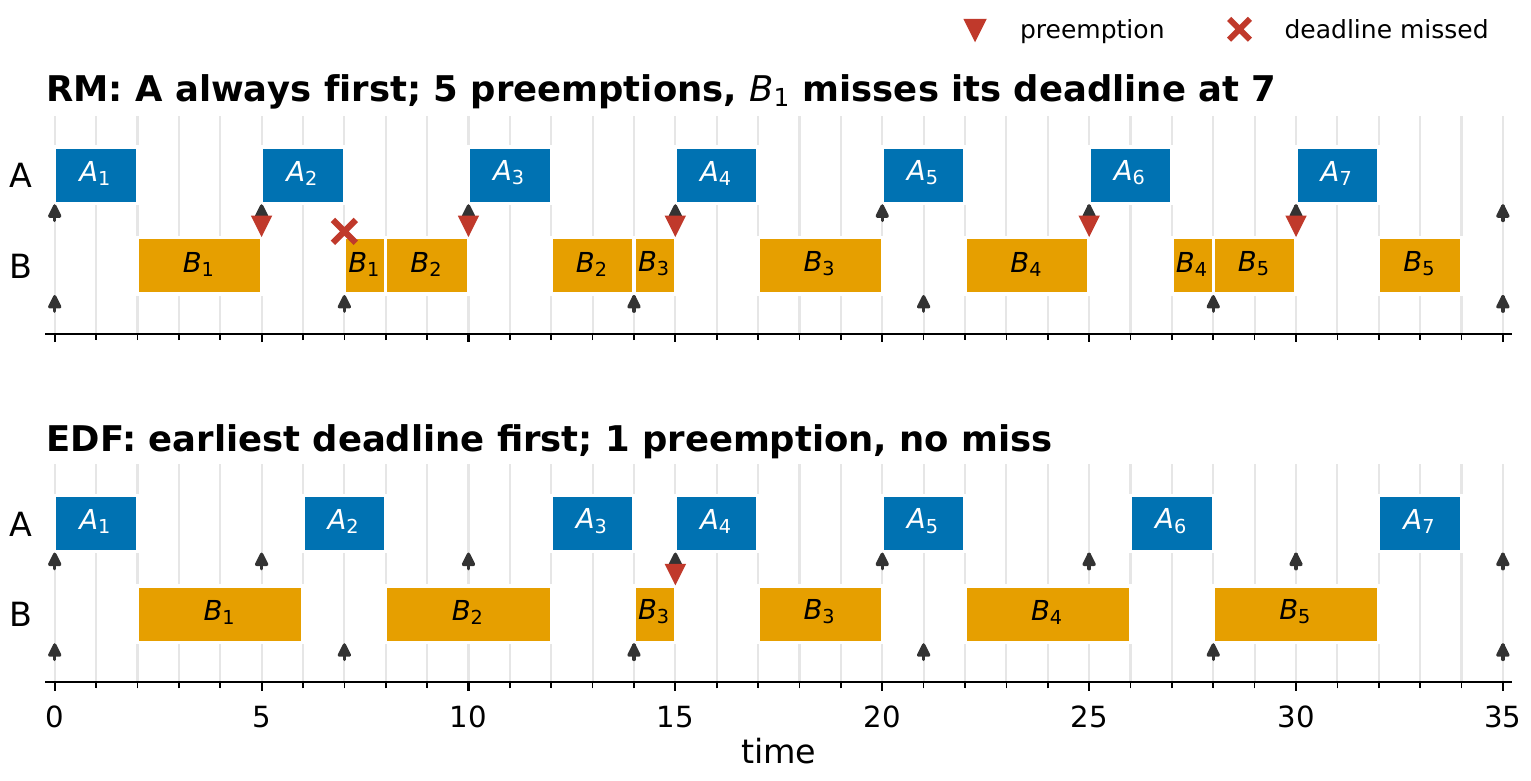
\includegraphics[width=\textwidth]{images/week-06/w6-u2-rm-vs-edf.png}
    \caption{RM and EDF on A ($C = 2, T = 5$) and B ($C = 4, T = 7$); triangles mark the preemptions. With RM, $A_2$ preempts $B_1$ at 5 and $B_1$ misses its deadline 7. With EDF, $B_1$ ($d = 7$) keeps the CPU against $A_2$ ($d = 10$) and no deadline is missed.}
\end{figure}

\subsection{Under overload: who misses?}
A ($C = 1, T = 3$), B ($C = 2, T = 4$), C ($C = 2, T = 6$):
\[
U = \frac{1}{3} + \frac{2}{4} + \frac{2}{6} = \frac{4}{12} + \frac{6}{12} + \frac{4}{12} = \frac{14}{12} = \frac{7}{6} = 1.167 > 1
\]
An \textbf{overload} (in a real system, often a task that runs longer than its WCET): no algorithm can meet every deadline. Two hyperperiods ($H = 12$):

\paragraph{RM:} only C, the \textbf{lowest} priority, misses (first at 6); A and B are never late.
\begin{verbatim}
    time  0         10        20
        |.........|.........|...
    A     #..#..#..#..#..#..#..#..
    B     .##.##..#.#..##.##..#.#.
    C     .......#...#.......#...#   <- C misses at 6, 12, 18, 24
    CPU   ABBABBACBABCABBABBACBABC
\end{verbatim}

\paragraph{EDF:} the first miss comes later (C at 12), but then A, B and C \textbf{all} miss.
\begin{verbatim}
    time  0         10        20
        |.........|.........|...
    A     #..#....##....#..#....##   <- A misses at 21
    B     .##...##..##...##...##..   <- B misses at 16, 20, 24
    C     ....##......##....##....   <- C misses at 12, 18, 24
    CPU   ABBACCBBAABBCCABBACCBBAA
\end{verbatim}
With EDF a late job keeps an early deadline and delays the next jobs, which become late too: a \textbf{domino effect}. With RM the damage stays in the lowest-priority tasks, so you choose which tasks may suffer: a \emph{graceful} degradation.
\begin{figure}[H]
    \centering
    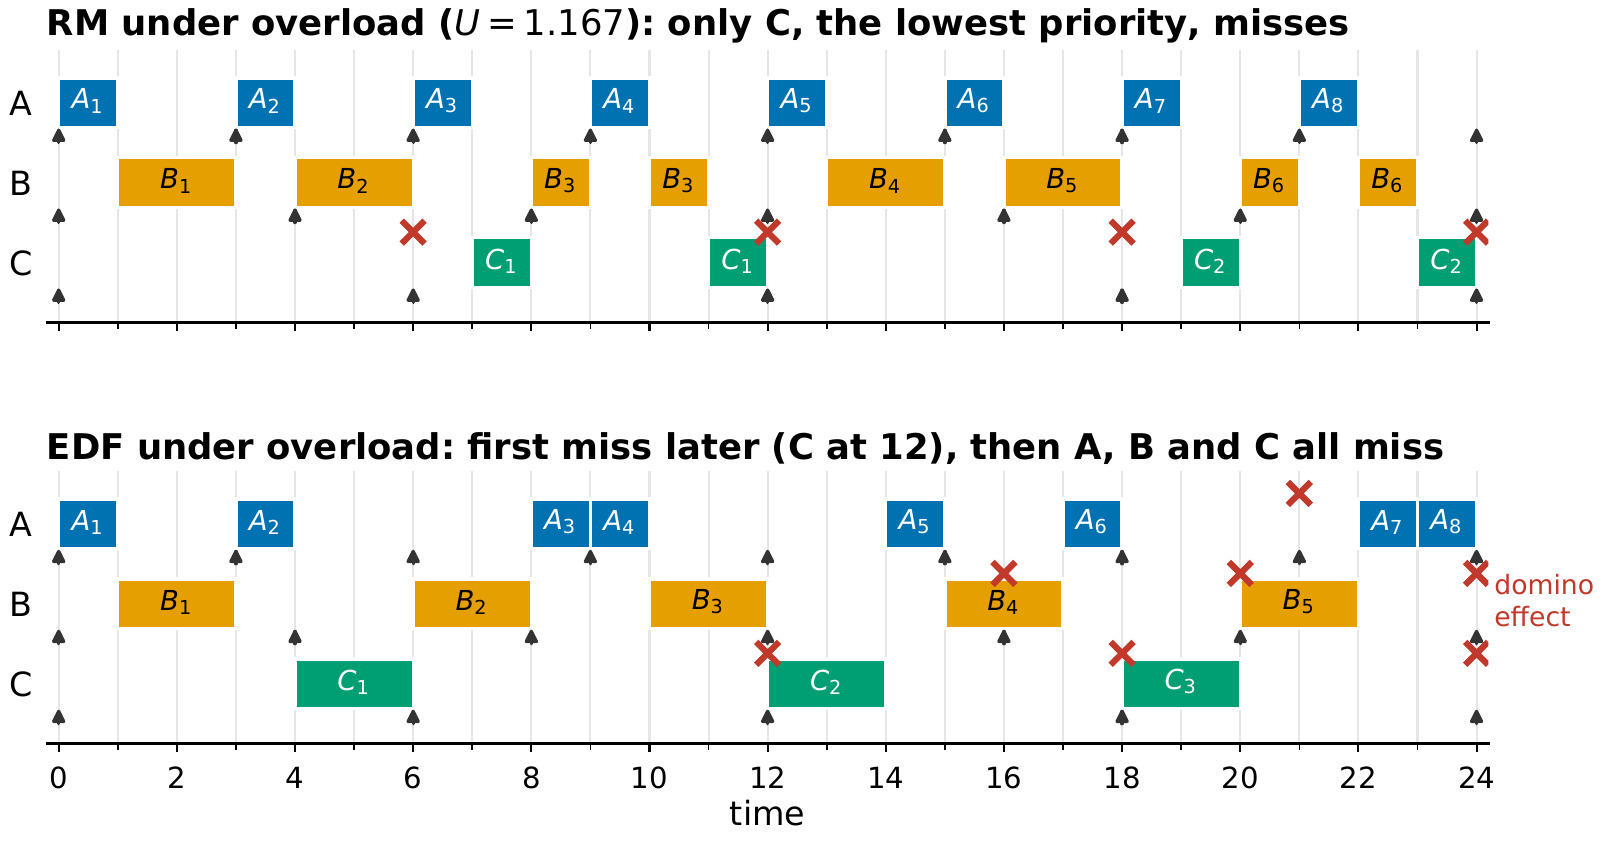
\includegraphics[width=\textwidth]{images/week-06/w6-u2-overload.png}
    \caption{Overload ($U = 1.167$) over two hyperperiods; crosses mark the missed deadlines. RM confines the damage to C, the lowest priority; with EDF the late jobs keep their early deadlines and delay all the others (domino effect).}
\end{figure}

\subsection{RM or EDF?}
\begin{center}
    \begin{tabular}{l p{5.5cm} p{5.5cm}}
        \hline
        & RM & EDF \\
        \hline
        Priority & fixed, from $T$, set once & dynamic, from $d$, per job \\
        Exact test & RTA, iterations per task & $U \le 1$ \\
        Usable CPU & up to $U_{lub}(n)$ ($\ge 69\%$), more if RTA says so & up to 100\% \\
        Implementation & any priority scheduler: most RTOS kernels offer only fixed priorities & must compute $d$ at each release and keep the ready jobs sorted by $d$ \\
        Run-time overhead & low: the priority never changes & higher work per release; often fewer preemptions \\
        Overload & predictable: the lowest priorities miss & domino effect: any task can miss \\
        \hline
    \end{tabular}
\end{center}
\begin{itemize}
    \item Choose \textbf{RM} when the set passes the bound or RTA, or when overload must hit only known, less important tasks.
    \item Choose EDF when RM fails and $U \le 1$: it uses the CPU fully, if the kernel supports it.
\end{itemize}

\paragraph{EDF in real products.} Although optimal, EDF is little used: every deadline is met, but the order of the tasks is hard to predict, and safety-critical products must be \textbf{certified} on paper, where \textbf{predictability} matters most. Many cars, airplanes, trains and medical devices use timeline scheduling, the most predictable (always the same order); many products use rate monotonic, which wastes less CPU. Some producers prefer a more powerful CPU with a less efficient algorithm to a less predictable one.

\subsection{Exercise: RM or EDF?}
System 1: A ($C = 2, T = 4$), B ($C = 3, T = 6$).
\begin{enumerate}
    \item Compute $U$ and apply the Liu--Layland test.
    \item Apply RTA to B. Is the set feasible with RM? If not, give \texttt{first\_miss}.
    \item Is it feasible with EDF? Draw both schedules over $H$.
\end{enumerate}
System 2: the RM worked example A (1, 4), B (1, 5), C (2, 10), $U = 0.650$, on a kernel that offers only fixed priorities. A rare bug may make C run longer than its WCET.
\begin{enumerate}
    \setcounter{enumi}{3}
    \item For each system: RM or EDF? Give one reason.
\end{enumerate}

\textbf{Solution.}
\begin{enumerate}
    \item $U = 2/4 + 3/6 = 1$ (1.000); $U_{lub}(2) = 0.828$; $1.000 > 0.828$: inconclusive.
    \item $R_A = 2$. B:
    \[
    R_B^{(0)} = 3, \quad R_B^{(1)} = 3 + \left\lceil \tfrac{3}{4} \right\rceil \cdot 2 = 5, \quad R_B^{(2)} = 3 + \left\lceil \tfrac{5}{4} \right\rceil \cdot 2 = 7 > 6
    \]
    $R_B = 7$, missed. RM: not feasible, \texttt{first\_miss=B@6}.
    \item EDF: $U = 1 \le 1$: feasible. $H = \mathrm{LCM}(4, 6) = 12$.
\begin{verbatim}
    RM
    time  0         10
        |.........|..
    A     ##..##..##..
    B     ..##..##..##   <- B1 misses its deadline at 6
    CPU   AABBAABBAABB

    EDF
    time  0         10
        |.........|..
    A     ##...##...##
    B     ..###..###..
    CPU   AABBBAABBBAA
\end{verbatim}
    RM: \texttt{schedule=AABBAABBAABB}; EDF: \texttt{schedule=AABBBAABBBAA}.
    \item System 1: EDF, the only one of the two that meets every deadline. System 2: RM: $0.650 \le 0.780$ passes the bound, the kernel has fixed priorities, and if C overruns only C (the lowest priority) is late.
\end{enumerate}

\section{One-shot jobs}
EDF is the last algorithm for periodic tasks. Work that is not periodic has a separate scheduler with its own queues: the algorithms below assume that all jobs are aperiodic, and Unit 3 combines the two kinds of work.

\subsection{Aperiodic jobs}
An aperiodic (\emph{one-shot}) job arrives once, at an irregular time not known in advance: a key press, a message from the network, an alarm. It has an execution time $C$ and, being real time, often a deadline.
\begin{itemize}
    \item The theory so far relies on the period: $U = \sum C/T$ (in the bound and in $U \le 1$) and the RTA term $\lceil R / T_j \rceil C_j$ use $T$. Without $T$, neither the returns of a job nor its interference can be bounded: no schedulability analysis, no guarantee. A scheduler can only try to \textbf{minimise how late} the jobs are.
    \item Two different problems, two answers:
    \begin{itemize}
        \item \textbf{only one-shot jobs}, all known (arrival $a$, $C$, deadline $D$): meet the deadlines, or be as little late as possible. Algorithms: \textbf{Jackson} and \textbf{Horn} (this unit);
        \item \textbf{mixed sets}, hard periodic tasks plus aperiodic jobs whose arrival is not known in advance: keep every periodic deadline and serve the aperiodic jobs \textbf{fast}. Algorithms: \textbf{background}, \textbf{polling server}, \textbf{deferrable server} (Unit 3).
    \end{itemize}
\end{itemize}
A one-shot job is written with an uppercase letter (A), as in \texttt{schedsim}.

\subsection{Lateness and maximum lateness}
For one-shot jobs we measure how late each job is. Job $J$ arrives at $a$, has relative deadline $D$, absolute deadline $d = a + D$, and finishes at $f$:
\begin{itemize}
    \item \textbf{Lateness} $L = f - d$ (week 5): $L \le 0$, the deadline is met (early: good); $L > 0$, late by $L$ units.
    \item \textbf{Maximum lateness} $L_{max} = \max L$ over all jobs: $L_{max} \le 0$ means \textbf{every} deadline is met, and the schedule is feasible. When some job must be late, a small $L_{max}$ still keeps all jobs close to their deadline.
\end{itemize}
For example, if the latest job D has $d = 8$ and finishes at 10, $L_D = 10 - 8 = 2$; if it is the largest lateness, $L_{max} = 2$ (the set comes back with Jackson's algorithm).

\subsection{Naming a scheduling problem: $\alpha \,|\, \beta \,|\, \gamma$}
Before designing an algorithm, \textbf{name the problem}: textbooks write it as $\alpha \,|\, \beta \,|\, \gamma$, a heavy notation for a simple idea.
\begin{itemize}
    \item $\alpha$, the \textbf{machine}: the number of processors (\texttt{1}, \texttt{3}, \dots). This course uses a single-core CPU, realistic on small embedded systems: $\alpha = 1$.
    \item $\beta$, the \textbf{tasks and resources}, the most important field: preemption allowed (\texttt{preem}) or not (\texttt{no preem}); all jobs arriving at the same time (\texttt{sync}) or at arbitrary times (empty field). Each choice is a different problem, with a different algorithm.
    \item $\gamma$, the \textbf{goal} to optimise: $L_{max}$ (minimise the maximum lateness, i.e.\ try to respect the deadlines), $\sum f_i$ (the sum of the finishing times), $\sum Late_i$ (the number of late jobs).
\end{itemize}
Examples: $3 \,|\, \textit{no preem} \,|\, \sum f_i$, three processors, no preemption, arbitrary arrivals, minimise the sum of the finishing times; $2 \,|\, \textit{sync} \,|\, \sum Late_i$, two processors, all jobs arrive at 0, minimise the number of late jobs. Theory studies every combination, even those that never occur in practice. On one processor, two problems arise in real systems, both minimising $L_{max}$:
\begin{itemize}
    \item $1 \,|\, \textit{sync} \,|\, L_{max}$: a quiet system suddenly receives a \textbf{burst} of jobs at the same time, e.g.\ the camera, radar and infrared sensor of a car all detect an obstacle and raise an interrupt, each service computing the distance within a deadline. Solved by Jackson (EDD): run the jobs in \textbf{non-decreasing deadline} order (that is, increasing deadline order).
    \item $1 \,|\, \textit{preem} \,|\, L_{max}$: interrupts arrive one by one, at times not known in advance, and every job has a deadline. Solved by Horn (EDF): whenever the scheduler runs, earliest absolute deadline first.
\end{itemize}
\begin{figure}[H]
    \centering
    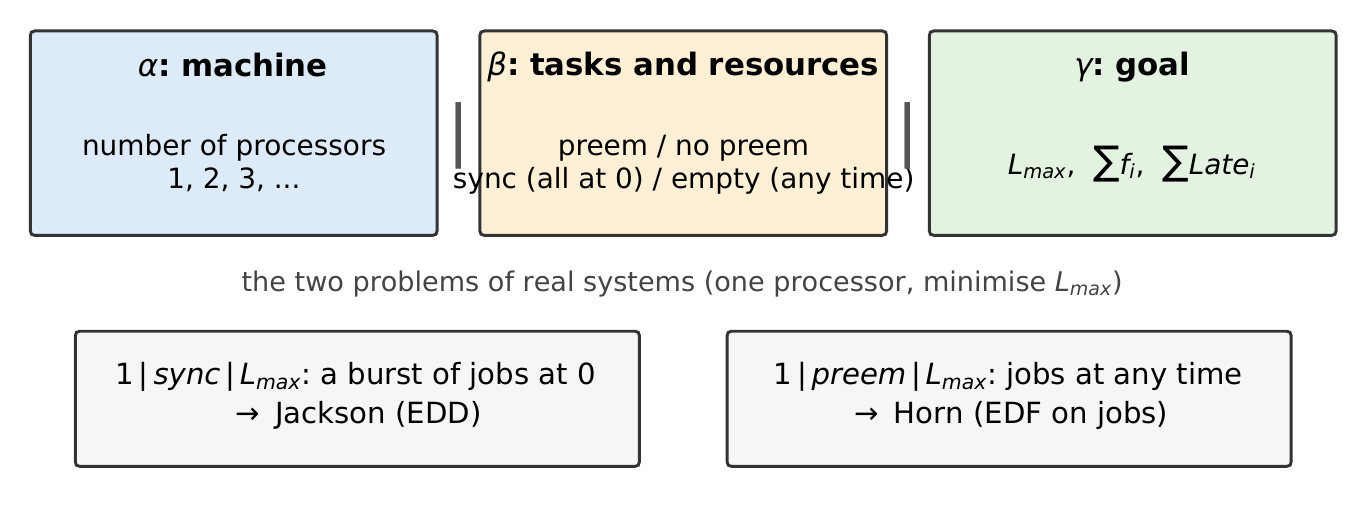
\includegraphics[width=0.92\textwidth]{images/week-06/w6-u2-notation.png}
    \caption{The $\alpha \,|\, \beta \,|\, \gamma$ notation, and the two problems of real systems solved in this unit.}
\end{figure}

\subsection{Jackson's algorithm (EDD)}
Problem $1 \,|\, \textit{sync} \,|\, L_{max}$: one processor, $n$ independent jobs that \textbf{all arrive at 0}, each with its own $C$ and $D$; minimise $L_{max}$.

\textbf{Earliest Due Date (EDD)}: run the jobs one after the other in order of non-decreasing deadline; same deadline, the lowest identifier first (course rule).
\begin{itemize}
    \item All jobs are there at 0, so preemption cannot help: EDD only fixes the order, sorting the jobs by $d$ before the start, and runs each job to the end.
    \item \textbf{Jackson's theorem}: EDD is optimal for $L_{max}$: no other order gives a smaller $L_{max}$.
    \item No guarantee that all deadlines can be met, but EDD settles it: with $L_{max} \le 0$ all are met; if EDD misses one ($L_{max} > 0$), every order misses one: the set is infeasible.
\end{itemize}

\subsection{Why EDD is optimal: swap two jobs}
Two jobs, both arriving at 0: A ($C = 2, D = 5$) and B ($C = 1, D = 2$). With two jobs, all orders can be tried.

\paragraph{Later deadline first, \texttt{AAB}.} A runs for 2 units, then B for 1:
\begin{verbatim}
    time  0  3
        |..|
    A     ##.
    B     ..#   <- B misses its deadline at 2
    CPU   AAB
\end{verbatim}
\[
L_A = 2 - 5 = -3 \ (\text{early}), \qquad L_B = 3 - 2 = 1, \qquad L_{max} = 1
\]
A positive $L_{max}$ means that at least one job misses its deadline: here B.

\paragraph{EDD, \texttt{BAA}.} Deadlines 2 and 5, so B first.
\begin{verbatim}
    time  0  3
        |..|
    A     .##
    B     #..
    CPU   BAA
\end{verbatim}
\[
L_B = 1 - 2 = -1, \qquad L_A = 3 - 5 = -2, \qquad L_{max} = -1
\]
No miss, and no other order does better.

\paragraph{The swap argument.} In any order, take a job X with a \textbf{later} deadline that runs just before a job Y with an earlier one, and swap them. The pair ends at the same time (3 in the example) and the other jobs do not move; Y finishes earlier, and X finishes where Y did, with a later deadline, so its lateness is not larger than Y's was. No swap increases $L_{max}$, and swapping until the order is EDD gives $L_{max}$ of EDD $\le$ $L_{max}$ of any order. Try four jobs with random times and deadlines in all orders: the best $L_{max}$ is always EDD's.
\begin{figure}[H]
    \centering
    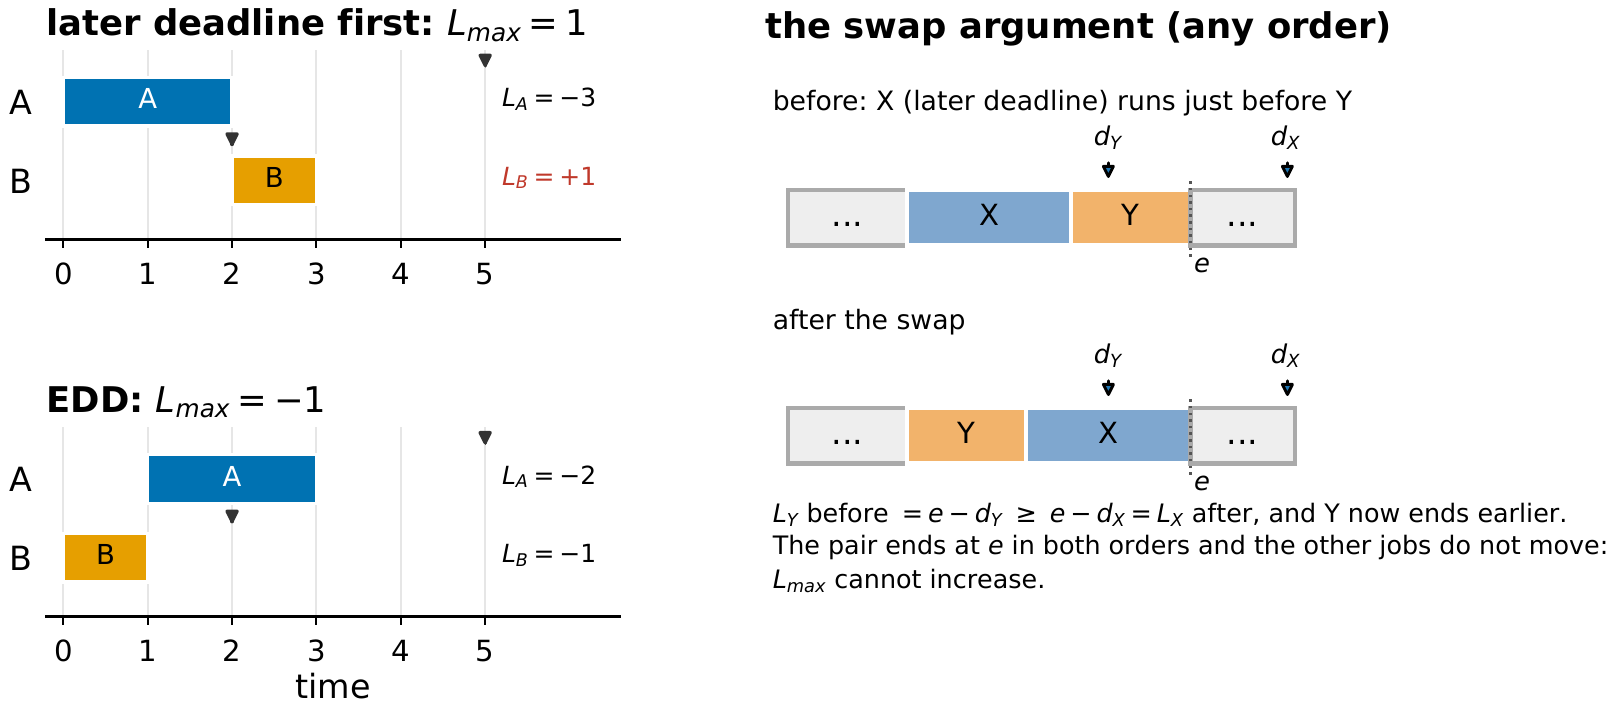
\includegraphics[width=\textwidth]{images/week-06/w6-u2-edd-swap.png}
    \caption{Left: the two orders of A ($C = 2, D = 5$) and B ($C = 1, D = 2$); arrows mark the deadlines. Right: the swap argument in general: exchanging an adjacent pair that runs the later deadline first never increases $L_{max}$.}
\end{figure}

\subsection{Jackson: worked example}
Five jobs, all arriving at 0 (so $d = D$):
\begin{center}
    \begin{tabular}{c | c c c c c}
        \hline
        job & A & B & C & D & E \\
        \hline
        $C$ & 1 & 1 & 1 & 3 & 2 \\
        $d$ & 3 & 10 & 7 & 8 & 5 \\
        \hline
    \end{tabular}
\end{center}
EDD order: A (3), E (5), C (7), D (8), B (10).
\begin{verbatim}
    time  0       8
        |.......|
    A     #.......
    B     .......#
    C     ...#....
    D     ....###.
    E     .##.....
    CPU   AEECDDDB
\end{verbatim}
\[
L_A = 1 - 3 = -2, \quad L_E = 3 - 5 = -2, \quad L_C = 4 - 7 = -3, \quad L_D = 7 - 8 = -1, \quad L_B = 8 - 10 = -2
\]
\texttt{schedule=AEECDDDB}, $L_{max} = L_D = -1 \le 0$: all deadlines met.

\paragraph{A case with a miss.} Five jobs, all arriving at 0:
\begin{center}
    \begin{tabular}{c | c c c c c}
        \hline
        job & A & B & C & D & E \\
        \hline
        $C$ & 1 & 2 & 1 & 4 & 2 \\
        $d$ & 2 & 5 & 4 & 8 & 6 \\
        \hline
    \end{tabular}
\end{center}
EDD order: A (2), C (4), B (5), E (6), D (8).
\begin{verbatim}
    time  0         10
        |.........|
    A     #.........
    B     ..##......
    C     .#........
    D     ......####   <- D misses its deadline at 8
    E     ....##....
    CPU   ACBBEEDDDD
\end{verbatim}
\[
L_A = -1, \quad L_C = -2, \quad L_B = -1, \quad L_E = 0, \quad L_D = 10 - 8 = 2
\]
\texttt{schedule=ACBBEEDDDD}, $L_{max} = 2$, \texttt{first\_miss=D@8}. EDD is optimal, so no order meets every deadline: only a faster CPU would help. Check: the total work is 10 units and no deadline is later than 8, so the job that runs last ends at 10, late.
\begin{figure}[H]
    \centering
    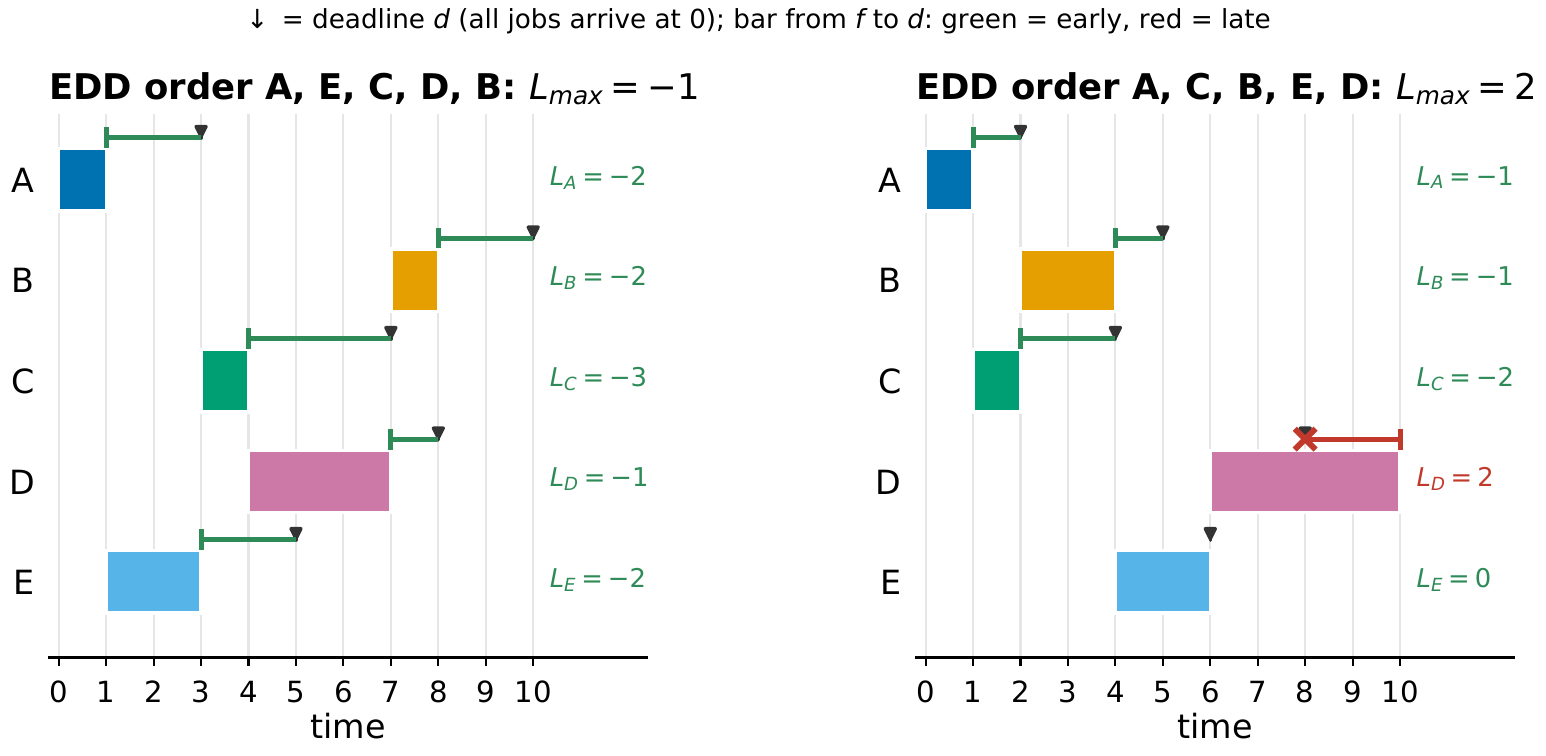
\includegraphics[width=\textwidth]{images/week-06/w6-u2-jackson.png}
    \caption{Jackson's algorithm on the two sets of this section. The bar between finish time and deadline shows the lateness, green when early, red when late. In the second set the total work (10 units) exceeds every deadline (at most 8), so the last job is late in any order.}
\end{figure}

\paragraph{Implementation.} At every activation of an aperiodic job (an interrupt, or whatever the design uses), the EDD scheduler \textbf{sorts} the ready aperiodic jobs by deadline and runs them one by one. Time 0 is the instant the burst arrives, with the whole set known, and deadlines are relative to it. Real systems often bend the assumptions of the theorem, and the result may no longer be optimal.

\paragraph{Aperiodic jobs in practice.} Jackson's algorithm assumes \textbf{no periodic tasks} (Unit 3 adds them). The future is unknown, so the analysis is a \textbf{worst-case} one: how many jobs can arrive together? With 25 interrupt lines, the worst case is all 25 at once, each with its deadline; if the CPU cannot cope with optimised code, a faster CPU is needed. Analysing only groups that fire together is possible, but no formula guarantees the outcome, as it does for periodic tasks: only the lateness measures the schedule. Hence the rule: \textbf{hard} real time is implemented with \textbf{periodic} tasks, \textbf{soft} real time is left to aperiodic jobs.

\subsection{Exercise: Jackson}
Five jobs, all arriving at 0, scheduled with Jackson's algorithm (EDD):
\begin{center}
    \begin{tabular}{c | c c c c c}
        \hline
        job & A & B & C & D & E \\
        \hline
        $C$ & 2 & 1 & 3 & 2 & 1 \\
        $D$ & 7 & 3 & 7 & 4 & 10 \\
        \hline
    \end{tabular}
\end{center}
\begin{enumerate}
    \item Write the EDD order. Two jobs have the same deadline: which one goes first?
    \item Draw the Gantt chart and write the schedule string.
    \item Compute the lateness of each job and $L_{max}$.
    \item Is the set feasible? If not, give \texttt{first\_miss}. Could another order do better?
\end{enumerate}

\textbf{Solution.}
\begin{enumerate}
    \item B (3), D (4), A (7), C (7), E (10). A and C both have $d = 7$: the lowest identifier, A, goes first.
    \item \begin{verbatim}
    time  0        9
        |........|
    A     ...##....
    B     #........
    C     .....###.   <- C misses its deadline at 7
    D     .##......
    E     ........#
    CPU   BDDAACCCE
\end{verbatim}
    \item $L_A = 5 - 7 = -2$, $L_B = 1 - 3 = -2$, $L_C = 8 - 7 = 1$, $L_D = 3 - 4 = -1$, $L_E = 9 - 10 = -1$; $L_{max} = 1$.
    \item In the answer format:
\begin{verbatim}
    schedule=BDDAACCCE
    L_A=-2
    L_B=-2
    L_C=1
    L_D=-1
    L_E=-1
    Lmax=1
    feasible=no
    first_miss=C@7
\end{verbatim}
    C ends at 8: $L_C = 1$. Swapping A and C gives $L_A = 8 - 7 = 1$: the same $L_{max}$. EDD is optimal: no order reaches $L_{max} \le 0$.
\end{enumerate}

\subsection{Horn's algorithm (EDF over jobs)}
Problem $1 \,|\, \textit{preem} \,|\, L_{max}$: one processor, jobs that arrive \textbf{at any time} (arrival $a$, $C$, $D$), preemption allowed; minimise $L_{max}$.

A new job may arrive while another runs: rather than waiting (first come, first served), to minimise the lateness the scheduler works \textbf{preemptively}, as EDF does: a job with a close deadline stops a running job with a far one, which resumes later.

\textbf{Horn's rule}: at every instant, run the ready job with the earliest absolute deadline $d = a + D$; a new job with a strictly earlier deadline preempts the running one.
\begin{itemize}
    \item This is EDF applied to one-shot jobs instead of periodic tasks. Ties: the week 5 rules.
    \item \textbf{Horn's theorem}: EDF is optimal for $L_{max}$, by the swap argument of Jackson applied to the slots of the schedule.
    \item Preemption is needed: a job with a near deadline may arrive while a long job runs. Without preemption, the problem with arbitrary arrivals is much harder.
    \item With all arrivals at 0 there is no preemption, and Horn gives the same schedule as Jackson.
\end{itemize}

\subsection{Horn: worked example}
Each job now also needs its \textbf{arrival time}. The table already gives the absolute deadline $d = a + D$:
\begin{center}
    \begin{tabular}{c | c c c c c}
        \hline
        job & A & B & C & D & E \\
        \hline
        $a$ & 0 & 0 & 2 & 3 & 6 \\
        $C$ & 1 & 2 & 2 & 2 & 2 \\
        $d = a + D$ & 2 & 5 & 4 & 10 & 9 \\
        \hline
    \end{tabular}
\end{center}
The scheduler decides at every arrival and completion:
\begin{itemize}
    \item $t = 0$: A and B are ready; A has the earlier deadline (2) and runs; at 1, B.
    \item $t = 2$: C arrives with $d = 4$ while B ($d = 5$) is running: C preempts B.
    \item $t = 3$: D arrives with $d = 10$, far away: C keeps running.
    \item $t = 4$: C completes; B ($d = 5$) runs before D ($d = 10$), which runs one unit at 5.
    \item $t = 6$: E arrives with $d = 9$, earlier than D's 10: E preempts D. After E (6--8), D resumes and finishes at 9.
\end{itemize}
\begin{verbatim}
    time  0        9
        |........|
    A     #........
    B     .#..#....
    C     ..##.....
    D     .....#..#
    E     ......##.
    CPU   ABCCBDEED
\end{verbatim}
\[
L_A = 1 - 2 = -1, \quad L_B = 5 - 5 = 0, \quad L_C = 4 - 4 = 0, \quad L_D = 9 - 10 = -1, \quad L_E = 8 - 9 = -1
\]
\texttt{schedule=ABCCBDEED}, $L_{max} = 0$: every deadline is met, and no other schedule does better ($L_{max} = 0$ or worse).
\begin{figure}[H]
    \centering
    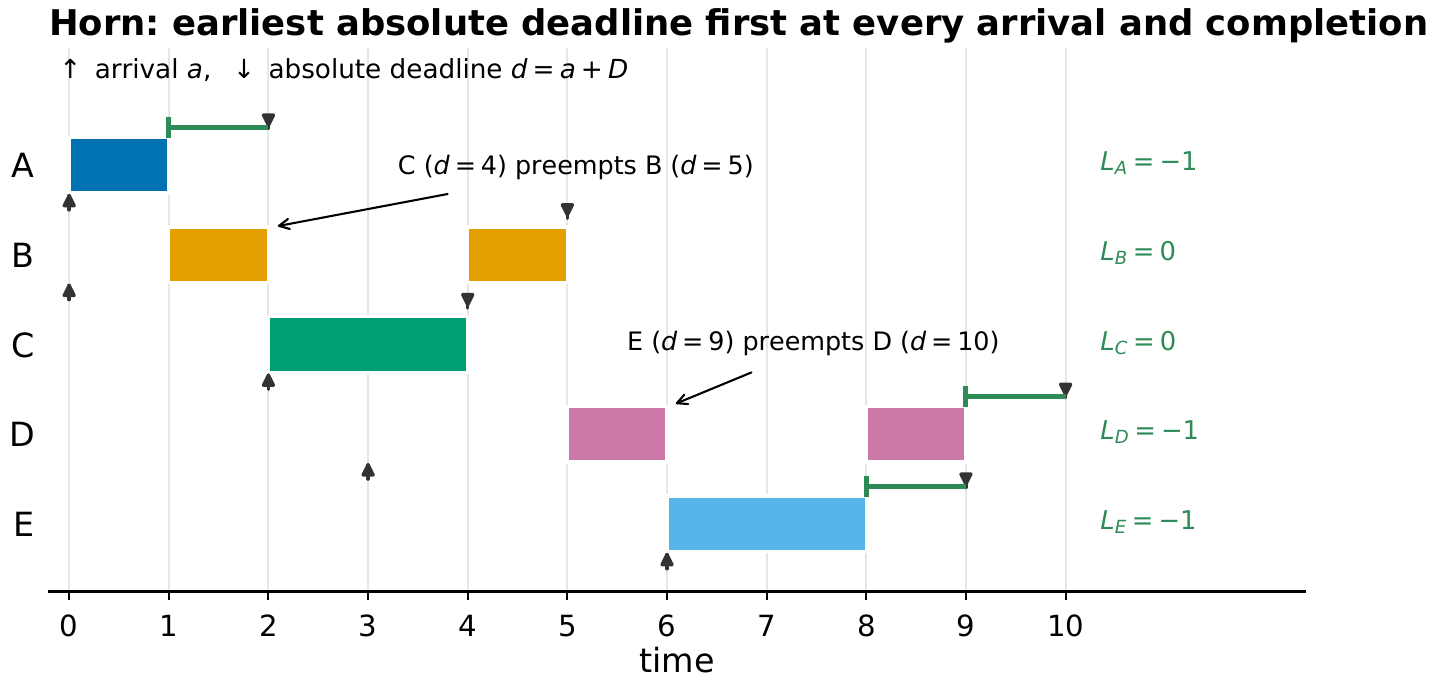
\includegraphics[width=0.88\textwidth]{images/week-06/w6-u2-horn.png}
    \caption{Horn's algorithm on the worked example: arrows below the rows mark the arrivals, arrows above the absolute deadlines. The two preemptions happen when a job with a strictly earlier deadline arrives.}
\end{figure}

\paragraph{Implementation.} The OS keeps the list of ready jobs and picks the earliest deadline, either keeping the list \textbf{ordered} (each new job inserted in place, e.g.\ in a linked list) or \textbf{unordered} and searched at every decision. That cost is the cost of the scheduler, and it is small: embedded systems run 10, 15 or 20 tasks, and a linear search over 20 elements is cheap.

\subsection{Exercise: Horn}
Five jobs, scheduled with Horn's algorithm. $D$ is relative: the absolute deadline is $d = a + D$.
\begin{center}
    \begin{tabular}{c | c c c c c}
        \hline
        job & A & B & C & D & E \\
        \hline
        arrival $a$ & 0 & 1 & 2 & 4 & 5 \\
        $C$ & 3 & 2 & 1 & 2 & 2 \\
        $D$ & 10 & 4 & 2 & 8 & 4 \\
        \hline
    \end{tabular}
\end{center}
\begin{enumerate}
    \item Compute the absolute deadline of each job.
    \item Draw the Gantt chart and write the schedule string. Where does a preemption happen?
    \item Compute the lateness of each job and $L_{max}$. Is the set feasible?
\end{enumerate}

\textbf{Solution.}
\begin{enumerate}
    \item $d$: A 10, B 5, C 4, D 12, E 9.
    \item B (5) preempts A (10) at 1; C (4) preempts B at 2; E (9) preempts A at 5. At 4, A (10) runs before D (12).
\begin{verbatim}
    time  0         10
        |.........|
    A     #...#..#..
    B     .#.#......
    C     ..#.......
    D     ........##
    E     .....##...
    CPU   ABCBAEEADD
\end{verbatim}
    \item $L_A = 8 - 10 = -2$, $L_B = 4 - 5 = -1$, $L_C = 3 - 4 = -1$, $L_D = 10 - 12 = -2$, $L_E = 7 - 9 = -2$; $L_{max} = -1 \le 0$: feasible.
\begin{verbatim}
    schedule=ABCBAEEADD
    L_A=-2
    L_B=-1
    L_C=-1
    L_D=-2
    L_E=-2
    Lmax=-1
    feasible=yes
    first_miss=none
\end{verbatim}
\end{enumerate}

\paragraph{Where we are now.} We can schedule only periodic tasks, or only aperiodic jobs; Unit 3 combines the two: the periodic tasks first, never missing a deadline, then the aperiodic jobs, not as plain best effort (where a job might never run) but so that each one surely runs. Apart from round robin, the course does not implement general-purpose (non-real-time) schedulers: embedded operating systems are mostly real time.

\section{Unit 2: summary}
\begin{itemize}
    \item \textbf{EDF}: the earliest absolute deadline runs; dynamic priorities, recomputed at every event; feasible if and only if $U \le 1$, so the CPU can be used at 100\%. Optimal on one CPU.
    \item \textbf{RM vs EDF}: EDF uses the whole CPU and saves sets that RM cannot; RM is simpler, in every RTOS, and predictable under overload, where EDF has a domino effect. Safety-critical products prefer timeline or RM.
    \item \textbf{Aperiodic} jobs have no period: $U$ and RTA do not apply, and deadlines cannot be guaranteed. One-shot jobs are judged by the lateness $L = f - d$ and $L_{max}$; $L_{max} \le 0$ means every deadline is met.
    \item $\alpha \,|\, \beta \,|\, \gamma$ names a problem: machine, task characteristics, goal.
    \item \textbf{Jackson (EDD)}, $1 \,|\, \textit{sync} \,|\, L_{max}$: all jobs at 0, run by non-decreasing deadline, no preemption. Optimal for $L_{max}$ (swap argument): if EDD misses, every order misses.
    \item \textbf{Horn (EDF)}, $1 \,|\, \textit{preem} \,|\, L_{max}$: jobs at any time, earliest absolute deadline first, with preemption. Optimal for $L_{max}$.
    \item In practice, hard real time is implemented with periodic tasks, soft real time is left to aperiodic jobs.
\end{itemize}

\section{Unità 3 - Mixed task sets: background, polling and deferrable servers}
Each algorithm so far assumes a single kind of work. This unit mixes periodic tasks and aperiodic jobs, and closes real-time scheduling.

\subsection{Mixed task sets}
Real systems mix \textbf{periodic tasks} (time-driven critical control loops with hard deadlines, Unit 1) and \textbf{aperiodic jobs} (event-driven: a button, a message, a fault; hard, soft or no deadline; arrival \textbf{not known} in advance). The goal: every periodic deadline \textbf{guaranteed}, and a \textbf{short response time} $R = f - a$ for the aperiodic jobs. The course uses one simple setup (more complex ones follow easily):
\begin{itemize}
    \item periodic tasks with RM, all released at 0, $D = T$, preemptible; another algorithm would work too, but fixed priorities keep the exercises simple;
    \item aperiodic jobs served \textbf{first come, first served} (same arrival: lowest identifier), deadlines ignored; with Jackson or Horn, only the policy of their queue would change;
    \item aperiodic jobs in \textbf{lowercase} (a), periodic tasks in \textbf{uppercase} (A), as in \texttt{schedsim}; one-shot jobs alone (Unit 2) stay uppercase;
    \item three ways to serve them, in increasing complexity and performance: background, polling server, deferrable server.
\end{itemize}

\subsection{Background scheduling}
The simplest approach: the periodic schedule usually leaves \textbf{idle time}, especially on a fast CPU, and the aperiodic jobs use it. \textbf{Background}: the periodic tasks run with RM; an aperiodic job runs \textbf{only when no periodic job is ready}.
\begin{itemize}
    \item An event such as an interrupt (very high priority) creates or activates the job and puts it in the aperiodic queue.
    \item Two ready queues, periodic (RM priority) and aperiodic (FCFS); the aperiodic one is served only when the periodic one is empty.
    \item Only the periodic scheduler decides: a periodic release preempts the aperiodic job at once.
\end{itemize}

\paragraph{Implementation.} Practically nothing to add: the \textbf{idle task} of the scratch-OS, which runs when there is nothing to do, reads the aperiodic queue and runs the jobs one by one; when the idle time ends, the scheduler gives the CPU back to the periodic tasks.
\begin{figure}[H]
    \centering
    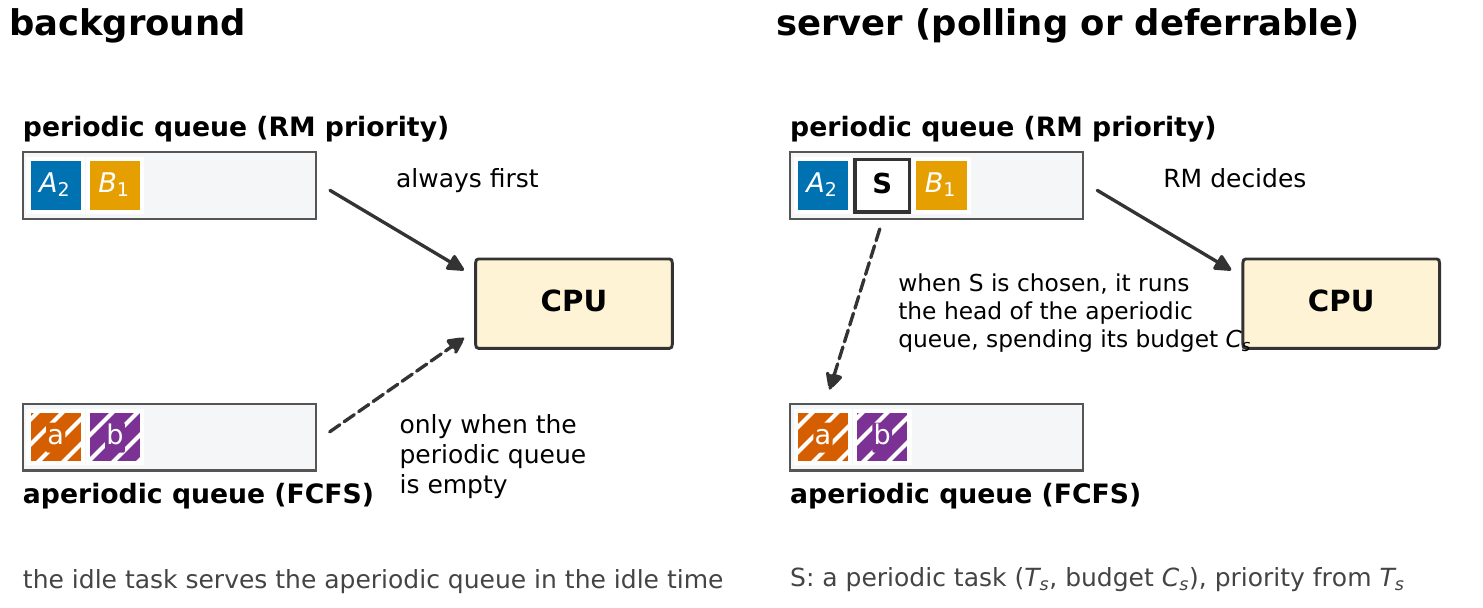
\includegraphics[width=\textwidth]{images/week-06/w6-u3-queues.png}
    \caption{Left: background service, where the aperiodic queue is served only when no periodic job is ready. Right: a server is one more entry of the RM queue; when it is chosen, it runs the head of the aperiodic queue and spends its budget.}
\end{figure}

\subsection{Background: worked example}
Periodic tasks A ($C = 2, T = 6$) and B ($C = 4, T = 10$), RM; aperiodic jobs a (arrives at 2, $C = 1$) and b (arrives at 12, $C = 2$), each with an arrival time and an execution time, no period. The analysis covers only the periodic tasks:
\[
U = \frac{2}{6} + \frac{4}{10} = \frac{10}{30} + \frac{12}{30} = \frac{22}{30} = \frac{11}{15} = 0.733 \le U_{lub}(2) = 0.828
\]
The set is RM-schedulable.

\paragraph{The periodic schedule.} A has the higher priority ($1/6 > 1/10$); A is released at 0, 6, 12, 18, B at 0, 10, 20. At 12 $A_3$ preempts B, which ends 14--16. RM leaves idle time at 8--10 and 16--18 (the chart covers 24 units).

\paragraph{The aperiodic jobs.} a arrives at 2, but a periodic job is ready until 8: it runs 8--9. b arrives at 12 and waits for the next idle time: 16--18.
\begin{verbatim}
    time  0         10        20
        |.........|.........|...
    A     ##....##....##....##....
    B     ..####....##..##....####
    a     ........#...............
    b     ................##......
    CPU   AABBBBAAa.BBAABBbbAABBBB
\end{verbatim}
\texttt{schedule=AABBBBAAa.BBAABBbbAABBBB}, \quad $R_a = 9 - 2 = 7$, \quad $R_b = 18 - 12 = 6$. The jobs ran only in the time left: a needs 1 unit and waits 6. With 3 units, b would wait for the next idle time, at 26 ($H = \mathrm{LCM}(6, 10) = 30$), and finish at 27 ($R_b = 15$).
\begin{figure}[H]
    \centering
    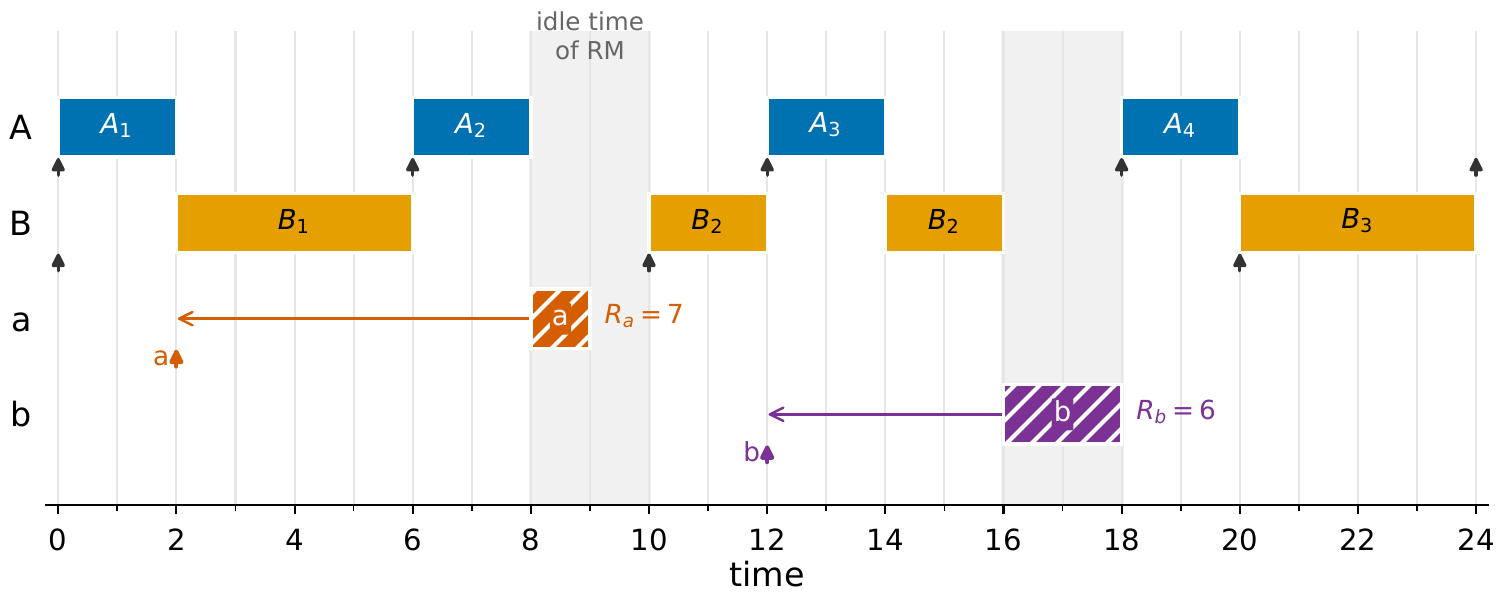
\includegraphics[width=\textwidth]{images/week-06/w6-u3-background.png}
    \caption{The background worked example: the aperiodic jobs run only in the idle time left by RM (grey bands).}
\end{figure}

\subsection{Background: pros and cons}
\paragraph{Pros.} Very simple: two ready queues, no new parameter. The periodic tasks, the important ones, are \textbf{not disturbed}: their schedule is \textbf{exactly} the RM schedule without the aperiodic jobs, and all the tests of Unit 1 stay valid. Idle time is used instead of wasted.

\paragraph{Cons.} The aperiodic response time is what the periodic load leaves: \textbf{very long} when $U$ is close to 1 (and a CPU is bought to be used), infinite with no idle time, and unbounded in general; aperiodic deadlines are ignored. Background fits only soft or non-real-time jobs (a late job loses its result but does no damage), on a CPU fast enough to leave idle time. Braking a car in background (never an aperiodic job anyway) would be unacceptable, above all on the single computer of new cars, which also plays videos and runs the air conditioning.

To serve aperiodic jobs earlier \textbf{and} still guarantee the periodic tasks, CPU time is reserved for them: a \textbf{server}.

\subsection{Exercise: background}
Periodic tasks A ($C = 1, T = 4$) and B ($C = 2, T = 8$) with RM. Aperiodic jobs in background: a arrives at 1 with $C = 2$, b arrives at 9 with $C = 3$. Horizon: 16.
\begin{enumerate}
    \item Compute $U$ and the Liu--Layland bound. What do they say?
    \item Compute $R_A$ and $R_B$ with RTA.
    \item Draw the Gantt chart for 16 units and write the schedule string.
    \item Compute the response time of a and b.
\end{enumerate}

\textbf{Solution.} As always, the schedulability analysis first, on the periodic tasks only.

(1) Two tasks, so the limit is $U_{lub}(2) = 0.828$:
\[
U = \frac{1}{4} + \frac{2}{8} = 0.500 \le 0.828
\]
RM-schedulable.

(2) A has the highest priority: $R_A = C_A = 1$. B iterates from its execution time:
\[
R_B^{(0)} = 2, \quad R_B^{(1)} = 2 + \left\lceil \tfrac{2}{4} \right\rceil \cdot 1 = 3, \quad R_B^{(2)} = 2 + \left\lceil \tfrac{3}{4} \right\rceil \cdot 1 = 3
\]
Fixed point, $R_B = 3$. Take the \textbf{ceiling before} multiplying by $C_j$: a common mistake. Both values are within the deadlines ($1 \le 4$, $3 \le 8$), as the bound said.

(3) The periodic tasks alone leave long idle times (B's period is 8):
\begin{verbatim}
    time  0         10
        |.........|.....
    A     #...#...#...#...
    B     .##......##.....
    CPU   ABB.A...ABB.A...
\end{verbatim}
a (arrival 1) takes the first idle slot, 3, is \textbf{preempted} by $A_2$ at 4, and finishes in 5--6; b (arrival 9) takes slot 11, waits for A at 12, and finishes in 13--15.
\begin{verbatim}
    time  0         10
        |.........|.....
    A     #...#...#...#...
    B     .##......##.....
    a     ...#.#..........
    b     ...........#.##.
    CPU   ABBaAa..ABBbAbb.
\end{verbatim}
(4) $R_a = 6 - 1 = 5$, \quad $R_b = 15 - 9 = 6$.
\begin{verbatim}
    schedule=ABBaAa..ABBbAbb.
    U=0.500
    bound=0.828
    R_A=1
    R_B=3
    R_a=5
    R_b=6
    feasible=yes
    first_miss=none
\end{verbatim}
No periodic deadline is missed and all the aperiodic jobs fit. They have no deadline here, since FCFS does not optimise their lateness anyway; with these arrival times, \textbf{Horn's} algorithm could reorder them to minimise it.

\subsection{The polling server}
Background leaves the aperiodic jobs out of the analysis. A good system \textbf{reserves} time for them with a server: a dummy periodic task, scheduled by RM like the others, that runs aperiodic jobs inside it. It has a period $T_s$ and, instead of a WCET, a \textbf{budget} (or \textbf{capacity}) $C_s$: the time it may spend on aperiodic jobs in each period. Like any task, it has a utilisation:
\[
U_s = \frac{C_s}{T_s}
\]
The two servers of this unit differ only in what happens when no aperiodic job is pending.

\paragraph{Server rules} (as in \texttt{Exam.md} and \texttt{schedsim}):
\begin{itemize}
    \item The server is scheduled with RM like the periodic tasks (or with EDF, in a more complex scheduler): its priority comes from $T_s$.
    \item With the same period as a task it has the same RM priority, but the task is more important, so in the tie the server counts as the highest identifier: if neither is running, the \textbf{task runs first}; a server that is already running keeps the CPU, as in Self-assessment 16.
    \item It is activated at $t = 0, T_s, 2T_s, \dots$ and runs other jobs, not itself. At each activation its budget is \textbf{recharged} to $C_s$ (with $C_s = 3$, every period starts with 3 units): it never accumulates.
    \item It runs only with budget and a pending aperiodic job; each slot costs 1 unit of budget. Unlike a periodic job, which runs until it ends, the server stops when its budget reaches 0.
\end{itemize}

\paragraph{Polling server rules.} A \textbf{polling} server is defined by how it loses its budget, the most important rule:
\begin{itemize}
    \item \textbf{No job pending at its activation}: the budget drops to 0 until the next period; a job arriving immediately after is too late.
    \item Its queue \textbf{becomes empty} while budget is left (the job was shorter than the budget): the rest of the budget is \textbf{lost}.
\end{itemize}
One exit condition, really: finding the queue empty, at its activation or after a job, ends the server's period, since it cannot know that a job will arrive one unit later. A job arriving during a period is served in \textbf{that} period only if the budget is still there (a job was pending at the activation, and the queue has not emptied); otherwise it waits for the \textbf{next} period. Other sources may implement polling slightly differently: this is the course rule, used in \texttt{Exam.md}, in \texttt{schedsim} and in the exercises. In the schedule, a server slot shows the name of the aperiodic job it runs.

\subsection{Polling server: worked example}
Periodic tasks A ($C = 1, T = 4$) and B ($C = 2, T = 6$); polling server $C_s = 2$, $T_s = 5$ (how to choose them is explained below). Priorities follow the periods, A (4) $>$ server (5) $>$ B (6): the period of the server sets the priority of the aperiodic jobs. Aperiodic jobs, as (arrival, $C$): a (2, 2), b (8, 1), c (12, 2), d (19, 1). The chart covers 24 units.
\begin{itemize}
    \item $t = 0$: no aperiodic job is pending: the budget drops to 0, and the first server period is lost; a, arriving at 2, waits for the next one.
    \item $t = 5$: new period, budget 2, a pending: a runs 5--7, $R_a = 7 - 2 = 5$; $B_2$, released at 6 with a lower priority, waits, runs at 7, is preempted by $A_3$ at 8, and finishes 9--10.
    \item $t = 10$: b (arrived at 8) is pending, so the budget is kept: b runs 10--11, $R_b = 11 - 8 = 3$. At 11 the queue is empty: the remaining unit is lost, although the period lasts until 15, so c (arriving at 12) waits.
    \item $t = 15$: c runs, is preempted by $A_5$ at 16, and ends at 18: $R_c = 18 - 12 = 6$.
    \item $t = 20$: d (arrived at 19) is pending: A runs at 20, d at 21, $R_d = 22 - 19 = 3$; at 22 the queue is empty and the rest of the budget is lost.
\end{itemize}
\begin{verbatim}
    time  0         10        20
        |.........|.........|...
    A     #...#...#...#...#...#...
    B     .##....#.#...##...##....
    a     .....##.................
    b     ..........#.............
    c     ...............#.#......
    d     .....................#..
    CPU   ABB.AaaBABb.ABBcAcBBAd..
\end{verbatim}
\texttt{schedule=ABB.AaaBABb.ABBcAcBBAd..}, \quad $R_a = 5$, $R_b = 3$, $R_c = 6$, $R_d = 3$.
\begin{figure}[H]
    \centering
    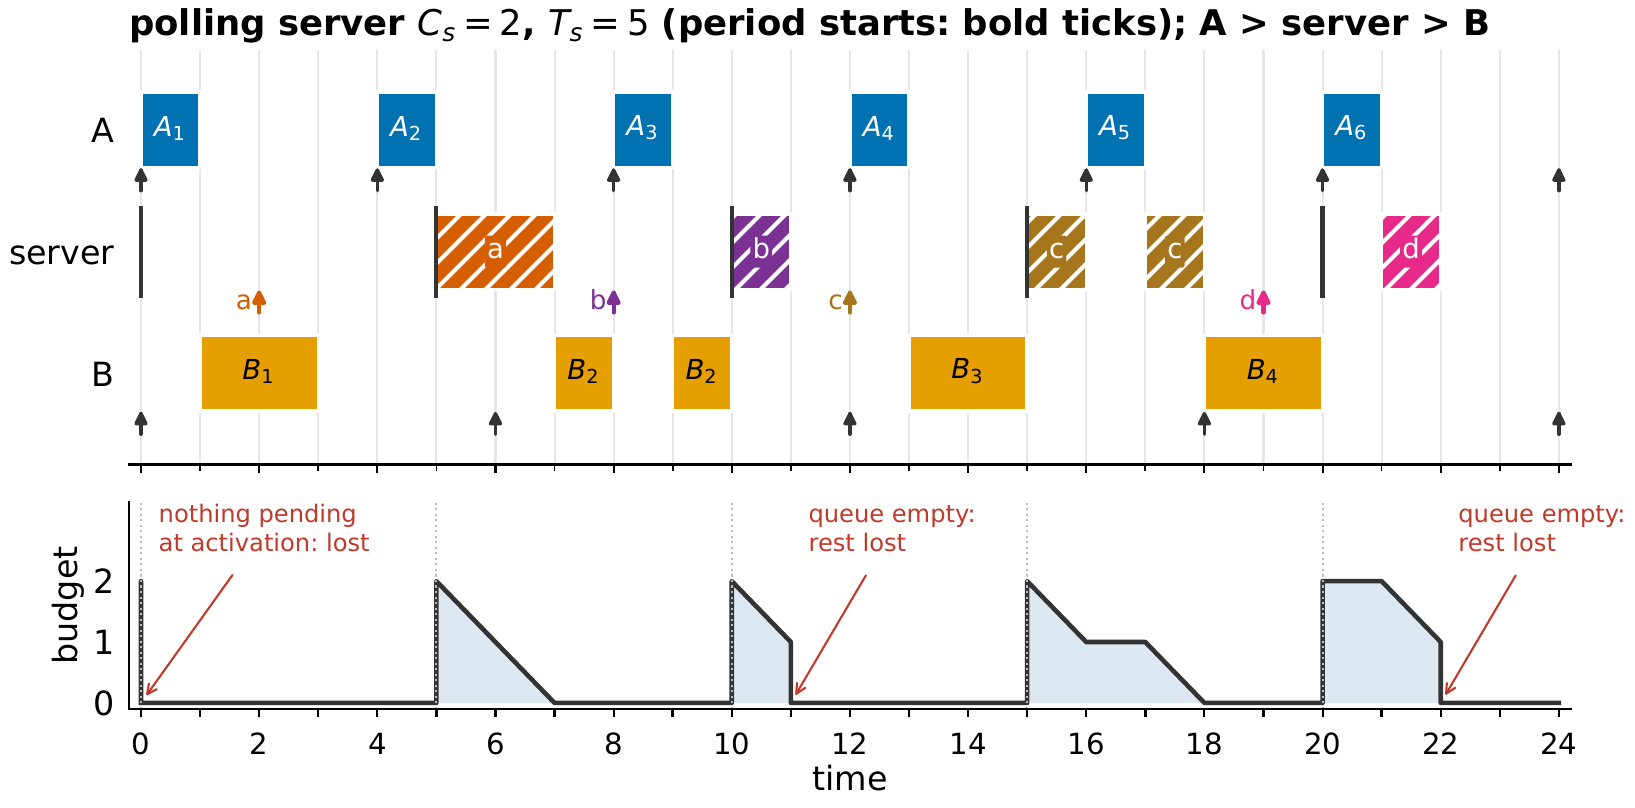
\includegraphics[width=\textwidth]{images/week-06/w6-u3-polling.png}
    \caption{The polling server worked example: schedule (bold ticks mark the server periods, arrows the arrivals of the aperiodic jobs) and budget. The budget is lost at an activation with nothing pending (at 0) and whenever the queue becomes empty (at 11 and 22).}
\end{figure}

\subsection{Polling server: the feasibility test}
A server is one more periodic task, $C_s$ every $T_s$, so the analysis of Unit 1 applies: with Liu--Layland the server is the third task (below $U_{lub}(3)$ the set is feasible, otherwise RTA can be tried). In the worked example:
\[
U + U_s = \frac{1}{4} + \frac{2}{6} + \frac{2}{5} = 0.583 + 0.400 = 0.983 > U_{lub}(3) = 0.780
\]
inconclusive. A related sufficient test, in \textbf{product} (hyperbolic) form, treats the server as one more task:
\[
\prod_{i=1}^{n} (U_i + 1) \cdot (U_s + 1) \le 2
\]
It never accepts less than the classic Liu--Layland form, often more, and it separates the server from the periodic tasks: for $n$ periodic tasks with $U_i = C_i / T_i$ and a polling server with $U_s = C_s / T_s$, the set is feasible with RM if
\[
P = \prod_{i=1}^{n} (U_i + 1) \le \frac{2}{U_s + 1}
\]
Like Liu--Layland, it is \textbf{sufficient} only: if it fails, the result is unknown. In the worked example $P = (1/4 + 1)(2/6 + 1) = 5/3 = 1.667$, $U_s = 2/5 = 0.400$, bound $2 / 1.4 = 1.429$: $1.667 > 1.429$, inconclusive, although no deadline is missed in the 24 units drawn.
\begin{figure}[H]
    \centering
    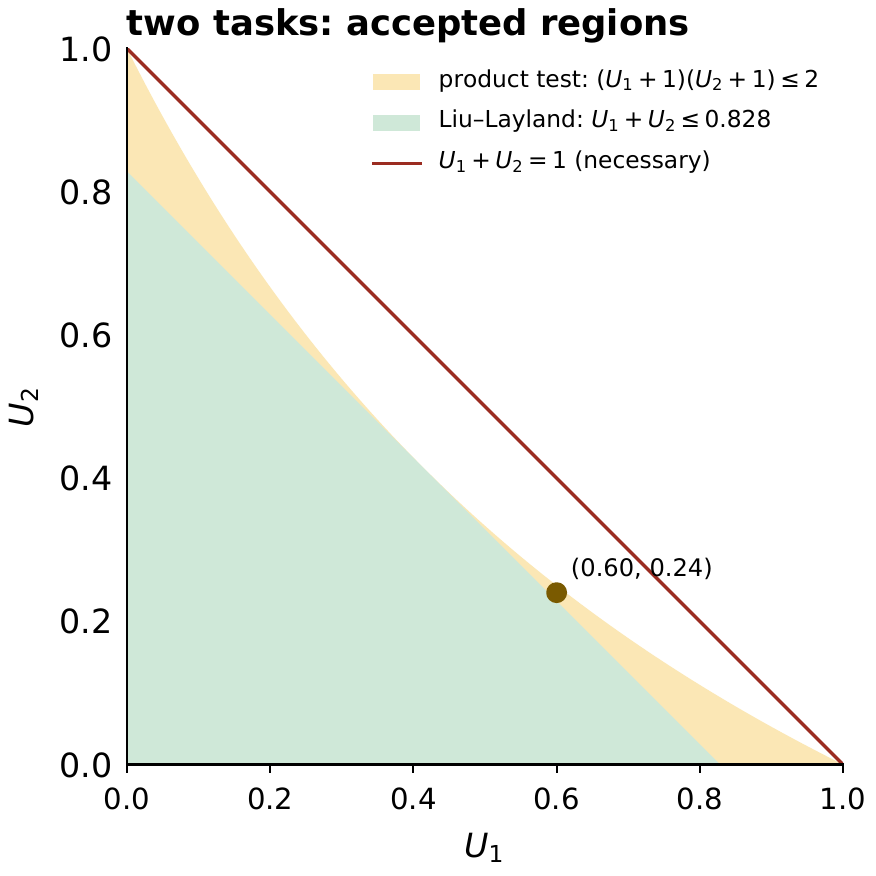
\includegraphics[width=0.5\textwidth]{images/week-06/w6-u3-hyperbolic.png}
    \caption{Two tasks: the region accepted by Liu--Layland ($U_1 + U_2 \le 0.828$) lies inside the region accepted by the product test ($(U_1 + 1)(U_2 + 1) \le 2$). A set such as $(0.60, 0.24)$, with $U = 0.84$, is accepted only by the product test.}
\end{figure}

\subsection{Sizing the polling server}
The test above is the design condition: the $U_i$ of the periodic tasks are known, $U_s$ is the unknown. Solving for $U_s$ gives the \textbf{largest server utilisation}, where the line $P$ meets the curve $2/(U_s + 1)$:
\[
P\,(U_s + 1) \le 2 \quad \Rightarrow \quad U_s \le \frac{2}{P} - 1 \quad \Rightarrow \quad U_{s,max} = \frac{2 - P}{P}
\]
$U_s$ is the ratio of two choices. The period $T_s$ sets the priority of the server: a shorter period gives more frequent activations and a higher priority to the aperiodic jobs, which matters when they handle important events. The budget $C_s$ is how long the server can run aperiodic jobs per period, never more than the period. It is a trade-off with no perfect rule. Rule of thumb: $T_s$ = the \textbf{shortest period}, so the server gets the highest priority (equal to that task, which wins the tie), and $C_s = U_s \cdot T_s$ with $U_s \le U_{s,max}$: at the exam, the largest \textbf{integer} $C_s$.

\paragraph{Example.} With A ($C = 1, T = 4$) and B ($C = 2, T = 6$), $P = 1.667$:
\[
U_{s,max} = \frac{2 - 1.667}{1.667} = \frac{0.333}{1.667} = 0.200
\]
With $T_s = 4$: $C_s \le 0.200 \times 4 = 0.8$, \textbf{no integer budget}. With $T_s = 10$ and $C_s = 2$ the test passes ($1.667 \le 2/1.2 = 1.667$), but the server has the lowest priority. The classic Liu--Layland form would give only $U_{s,max} = U_{lub}(3) - U = 0.780 - 0.583 = 0.197$, and with $T_s = 10$ it would allow only $C_s = 1$. Once the period and the budget of the server are chosen, the set is a normal rate-monotonic set.

\subsection{Exercise: polling server}
Periodic tasks A ($C = 1, T = 4$) and B ($C = 1, T = 8$) with RM. Polling server $C_s = 1$, $T_s = 4$. Aperiodic jobs: a arrives at 1 with $C = 2$, b arrives at 9 with $C = 1$. Horizon: 16.
\begin{enumerate}
    \item Compute $U$, $U_s$, $P$ and the bound $2/(U_s + 1)$. Does the test pass?
    \item Compute $U_{s,max}$. With $T_s$ = the shortest period, what is the largest integer $C_s$?
    \item Draw the Gantt chart for 16 units, and write the schedule string. The server and A have the same period: who wins the tie?
    \item Compute the response time of a and b.
\end{enumerate}

\textbf{Solution.}
\begin{enumerate}
    \item $U = 1/4 + 1/8 = 0.375$, $U_s = 1/4 = 0.250$, $P = (1.25)(1.125) = 1.406 \le 2 / 1.25 = 1.600$: guaranteed.
    \item $U_{s,max} = (2 - 1.406) / 1.406 = 0.594 / 1.406 = 0.422$; with $T_s = 4$, $C_s \le 1.69$: $C_s = 1$.
    \item At 0 nothing is pending: the budget is lost. A wins the tie at 4 and at 8 (the task runs before the server): a runs at 5 and at 9. b arrives at 9, when the budget of the period 8--12 has just been used by a: it waits for the period at 12, and runs after A.
\begin{verbatim}
    time  0         10
        |.........|.....
    A     #...#...#...#...
    B     .#........#.....
    a     .....#...#......
    b     .............#..
    CPU   AB..Aa..AaB.Ab..
\end{verbatim}
    \item $R_a = 10 - 1 = 9$, $R_b = 14 - 9 = 5$.
\begin{verbatim}
    schedule=AB..Aa..AaB.Ab..
    U=0.375
    Us=0.250
    P=1.406
    bound=1.600
    Usmax=0.422
    R_a=9
    R_b=5
    feasible=yes
    first_miss=none
\end{verbatim}
\end{enumerate}

\subsection{The deferrable server}
The polling server wastes its budget when no job is pending at the right moment, so a job arriving just after waits a whole period. The \textbf{deferrable server} \textbf{keeps} its budget until the end of the period, even with nothing to do; the rest is as for the polling server: same parameters, same RM priority from $T_s$, same tie rule. It serves an aperiodic job \textbf{at any time} while budget is left, so an arriving job can preempt a lower-priority task at once; at each period start the budget is set \textbf{back to} $C_s$, not added to what is left.

\subsection{Polling vs deferrable: the budget}
Both servers with $C_s = 2$, $T_s = 5$, and one aperiodic job a, arriving at 2 with $C = 1$:
\begin{itemize}
    \item \textbf{Polling}: nothing is pending at 0, so the budget drops to 0; at 5 it is recharged, a runs 5--6, and the rest of the budget is lost. $R_a = 6 - 2 = 4$.
    \item \textbf{Deferrable}: the budget stays, and a runs at once, 2--3: $R_a = 3 - 2 = 1$. The remaining unit is kept until the end of the period: a job arriving at 4 could still use it.
\end{itemize}
The deferrable server is a bit harder to implement, since it must be woken up at every aperiodic activation, but it uses the reserved time better, with less idle time.
\begin{figure}[H]
    \centering
    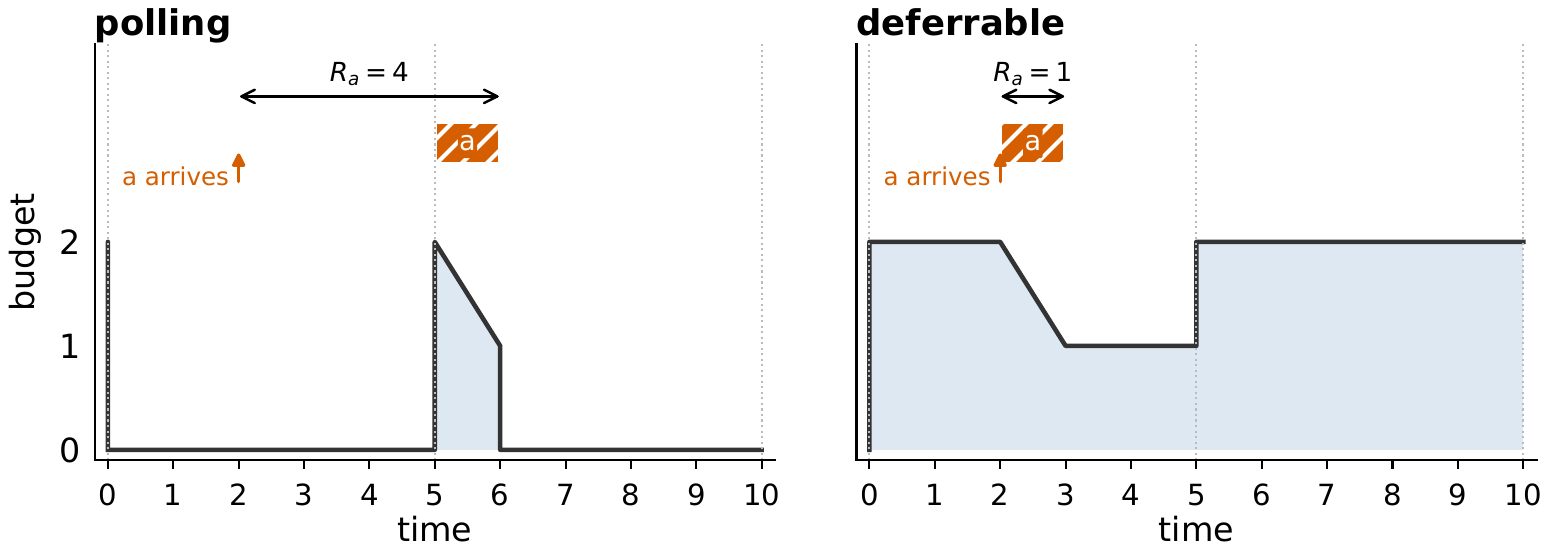
\includegraphics[width=\textwidth]{images/week-06/w6-u3-polling-vs-deferrable.png}
    \caption{Budget of the two servers for a single job a arriving at 2: the polling server has already lost its budget, so a waits for the next period; the deferrable server serves it at once.}
\end{figure}

\subsection{Deferrable server: worked example}
The same set as the polling example: A ($C = 1, T = 4$), B ($C = 2, T = 6$), server $C_s = 2$, $T_s = 5$, aperiodic a (2, 2), b (8, 1), c (12, 2), d (19, 1); A $>$ server $>$ B; 24 units.
\begin{itemize}
    \item $t = 0$: A runs; the budget of the first period, lost by the polling server, is kept. At 1 the server has budget but no job: B runs.
    \item $t = 2$: a arrives; the server has budget and a higher priority than B, so a preempts B and runs 2--4: $R_a = 4 - 2 = 2$.
    \item $t = 9$: b (arrived at 8, while A ran) is served at once: nothing of the period 5--10 was consumed, so the full budget is there, with one unit of time left in the period: $R_b = 10 - 8 = 2$.
    \item $t = 13$: c (arrived at 12) runs 13--15, right after A, on the budget of the period 10--15, kept until then: $R_c = 15 - 12 = 3$.
    \item $t = 19$: d preempts B at once: $R_d = 20 - 19 = 1$.
\end{itemize}
\begin{verbatim}
    time  0         10        20
        |.........|.........|...
    A     #...#...#...#...#...#...
    B     .#...###.......#.##..#..
    a     ..##....................
    b     .........#..............
    c     .............##.........
    d     ...................#....
    CPU   ABaaABBBAb..AccBABBdAB..
\end{verbatim}
\texttt{schedule=ABaaABBBAb..AccBABBdAB..}
\begin{center}
    \begin{tabular}{l | c c c c | c}
        \hline
        $R$ & a & b & c & d & avg \\
        \hline
        polling & 5 & 3 & 6 & 3 & 4.25 \\
        deferrable & \textbf{2} & \textbf{2} & \textbf{3} & \textbf{1} & \textbf{2.00} \\
        \hline
    \end{tabular}
\end{center}
Compared with the polling example, the deferrable server keeps its capacity available much longer.
\begin{figure}[H]
    \centering
    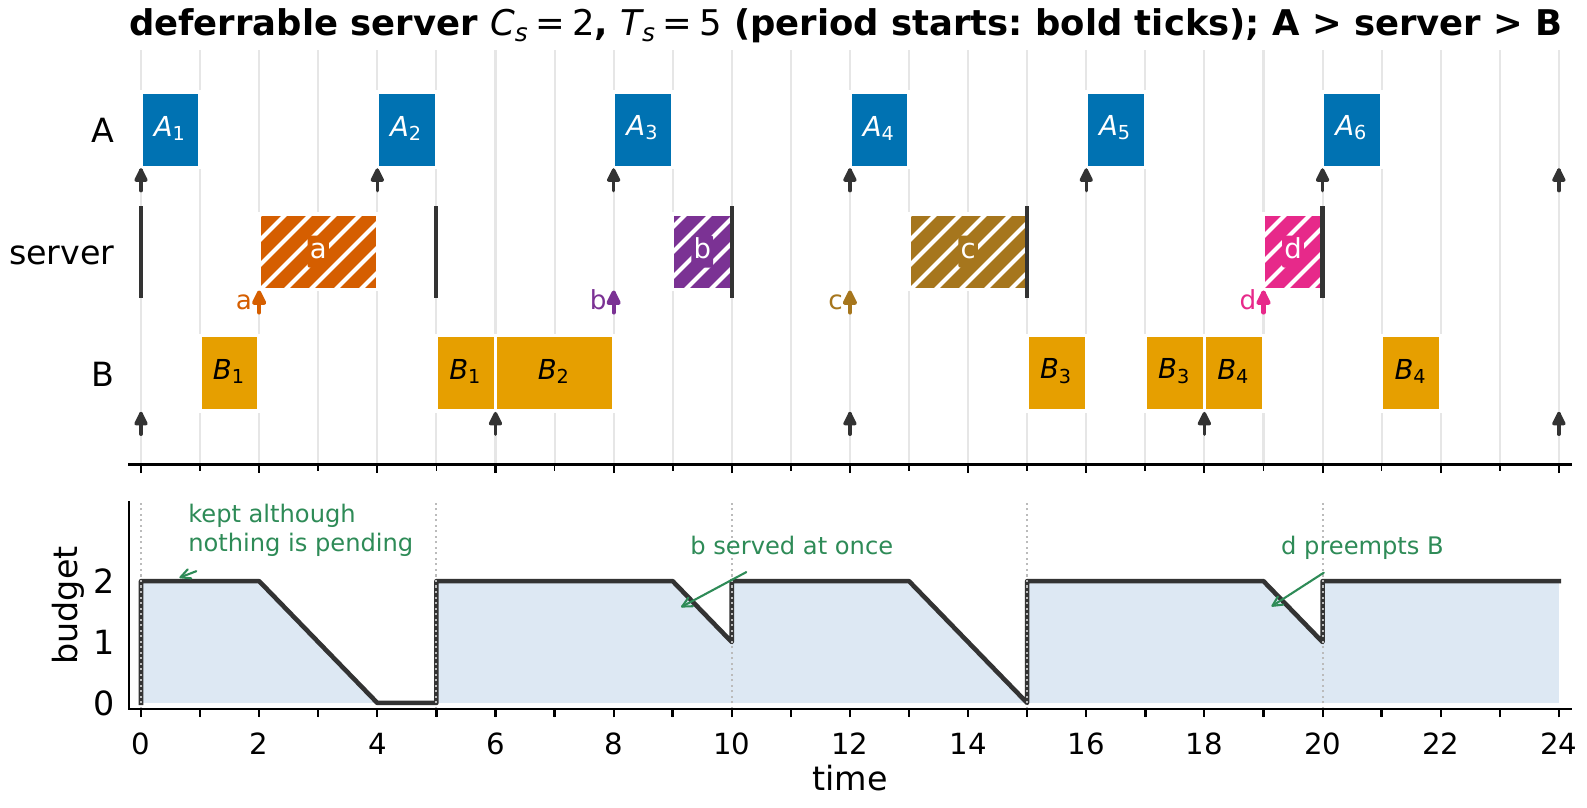
\includegraphics[width=\textwidth]{images/week-06/w6-u3-deferrable.png}
    \caption{The deferrable server on the same set as the polling example: the budget is kept until the end of each period, so each job is served as soon as the higher-priority work allows.}
\end{figure}

\subsection{The price: back-to-back execution}
The deferrable server can use its budget at the \textbf{end} of one period and again at the \textbf{start} of the next: up to $2C_s$ in a row. A ($C = 3, T = 6$), server $C_s = 2$, $T_s = 4$ (higher priority), a at 2 and b at 4, both with $C = 2$.

\paragraph{Deferrable:} a runs 2--4 (budget of the first period), b runs 4--6 (budget of the second). $A_1$ ends at 7: it \textbf{misses} its deadline 6.
\begin{verbatim}
    time  0         10
        |.........|..
    A     ##....####..   <- A1 misses its deadline at 6
    a     ..##........
    b     ....##......
    CPU   AAaabbAAAA..
\end{verbatim}
\paragraph{Polling:} the budget is lost at 0, a runs at 4, b at 8. No miss, but $R_a = 4$, $R_b = 6$ (deferrable: 2 and 2).
\begin{verbatim}
    time  0         10
        |.........|..
    A     ###...##..#.
    a     ....##......
    b     ........##..
    CPU   AAA.aaAAbbA.
\end{verbatim}
\begin{figure}[H]
    \centering
    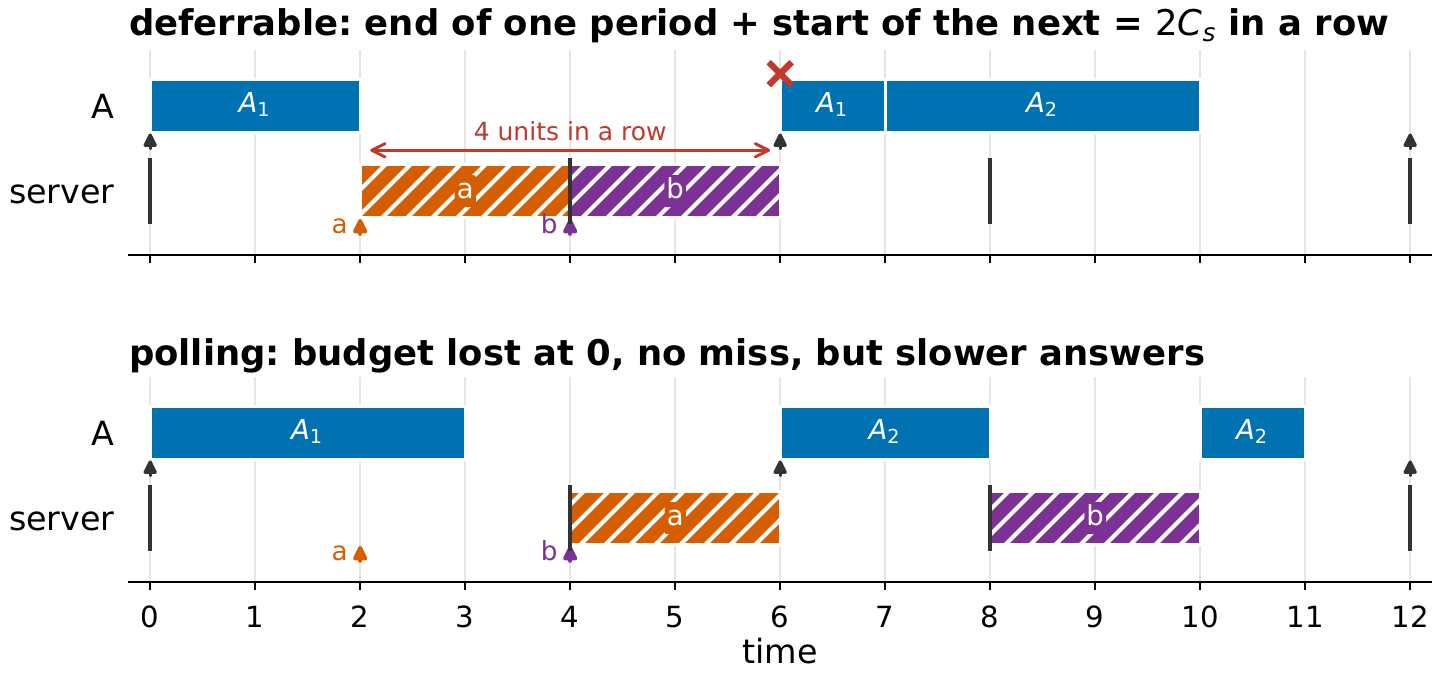
\includegraphics[width=0.92\textwidth]{images/week-06/w6-u3-back-to-back.png}
    \caption{Back-to-back execution: the deferrable server spends the budget of one period at its end (2--4) and the new budget at the start of the next (4--6), 4 units in a row, and $A_1$ misses its deadline at 6. The polling server avoids the miss, but answers later.}
\end{figure}

\subsection{Deferrable server: test and sizing}
Since it can run $2C_s$ in a row, the deferrable server is not a plain periodic task: it has its own test, again sufficient only and in product form (no need to derive it):
\[
P = \prod_{i=1}^{n} (U_i + 1) \le \frac{U_s + 2}{2U_s + 1}
\]
Here $P$ is the product over the $n$ periodic tasks ($U_i = C_i / T_i$; the server is not in it) and $U_s = C_s / T_s$: on the left the known periodic load, on the right the room left by a server of size $U_s$. Same shape as the polling bound $2/(U_s + 1)$, but \textbf{lower}: equal at $U_s = 0$ (2) and $U_s = 1$ (1), below in between.

\paragraph{Sizing.} As for polling, the largest server utilisation is where the line $P$ meets the curve: set the two sides equal and solve for $U_s$,
\[
P = \frac{U_s + 2}{2U_s + 1} \;\Rightarrow\; P(2U_s + 1) = U_s + 2 \;\Rightarrow\; U_s(2P - 1) = 2 - P \;\Rightarrow\; U_{s,max} = \frac{2 - P}{2P - 1}
\]
then choose $T_s$ and $C_s$ as for the polling server. In the worked example (A: $C = 1, T = 4$; B: $C = 2, T = 6$; server $C_s = 2, T_s = 5$):
\[
\begin{aligned}
&P = 1.667, \quad U_s = 0.400, \quad \text{bound} = \frac{0.4 + 2}{0.8 + 1} = \frac{2.4}{1.8} = 1.333, \quad 1.667 > 1.333: \text{inconclusive} \\
&U_{s,max} = \frac{2 - 1.667}{2 \cdot 1.667 - 1} = \frac{0.333}{2.333} = 0.143 \\
&T_s = 4: \ C_s \le 0.143 \cdot 4 = 0.571: \text{no integer budget passes}
\end{aligned}
\]
$U_{s,max} = 0.143$ is below the polling 0.200: the deferrable server answers faster, but leaves less room in the guarantee.
\begin{figure}[H]
    \centering
    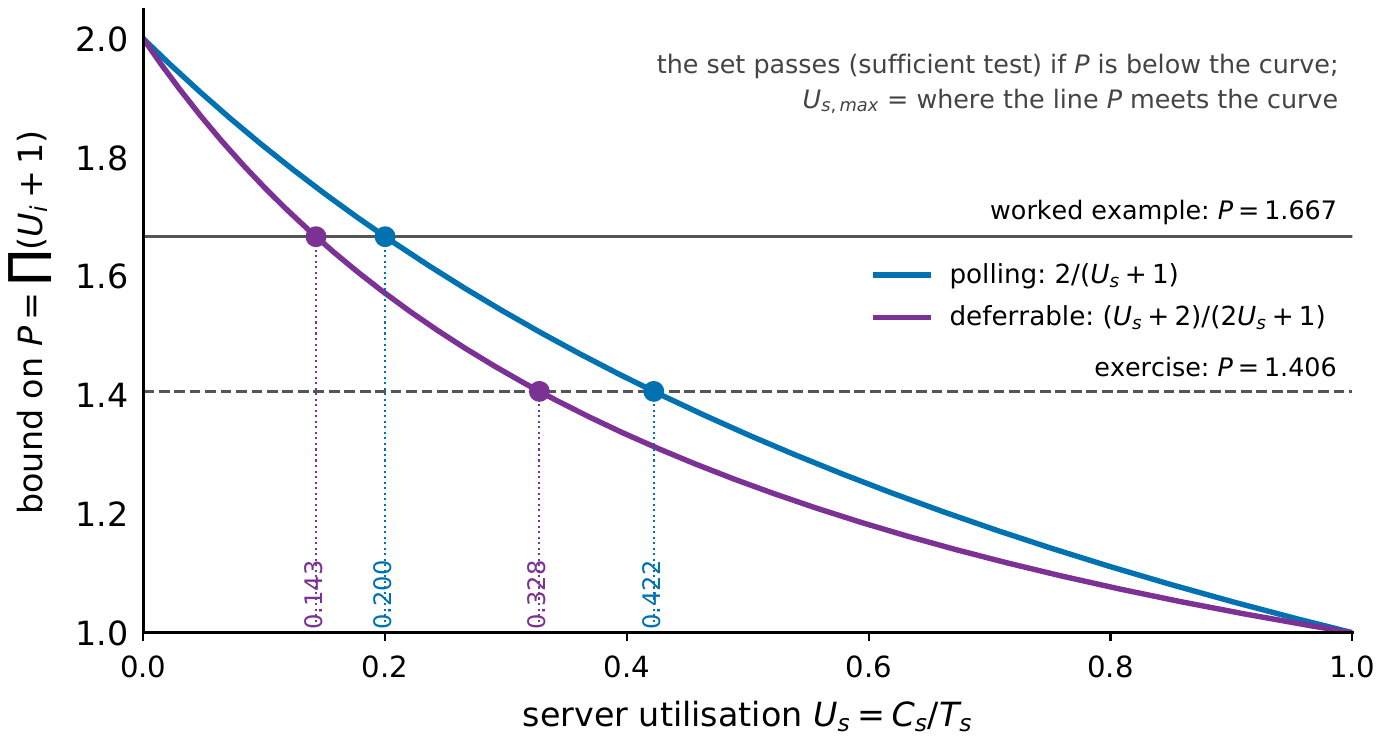
\includegraphics[width=0.88\textwidth]{images/week-06/w6-u3-server-bounds.png}
    \caption{The two server tests as functions of $U_s$. A set passes when its $P = \prod (U_i + 1)$ lies below the curve; $U_{s,max}$ is where the line $P$ meets the curve: 0.200 (polling) and 0.143 (deferrable) for the worked example, 0.422 and 0.328 for the exercise.}
\end{figure}

\subsection{Exercise: deferrable server}
The same set as the polling exercise, now with a deferrable server: A ($C = 1, T = 4$) and B ($C = 1, T = 8$) with RM, deferrable server $C_s = 1$, $T_s = 4$, a arrives at 1 with $C = 2$, b arrives at 9 with $C = 1$. Horizon: 16.
\begin{enumerate}
    \item Compute $U_s$, $P$ and the bound $(U_s + 2)/(2U_s + 1)$. Does the test pass?
    \item Compute $U_{s,max}$ and the largest integer $C_s$ with $T_s = 4$.
    \item Draw the Gantt chart for 16 units, and write the schedule string.
    \item Compute the response time of a and b, and compare them with the polling server.
\end{enumerate}

\textbf{Solution.}
\begin{enumerate}
    \item $U_s = 0.250$, $P = 1.406 \le (0.25 + 2) / 1.5 = 1.500$: guaranteed.
    \item $U_{s,max} = 0.594 / 1.812 = 0.328$; $C_s \le 1.31$: $C_s = 1$.
    \item a arrives at 1 with budget 1: it runs at once (the server is above B). At 4 the budget is back to 1, A wins the tie, and a ends at 6. b arrives at 9: the budget kept since 8 serves it at once.
\begin{verbatim}
    time  0         10
        |.........|.....
    A     #...#...#...#...
    B     ..#.......#.....
    a     .#...#..........
    b     .........#......
    CPU   AaB.Aa..AbB.A...
\end{verbatim}
    \item $R_a = 6 - 1 = 5$, $R_b = 10 - 9 = 1$, against 9 and 5 with polling.
\begin{verbatim}
    schedule=AaB.Aa..AbB.A...
    U=0.375
    Us=0.250
    P=1.406
    bound=1.500
    Usmax=0.328
    R_a=5
    R_b=1
    feasible=yes
    first_miss=none
\end{verbatim}
\end{enumerate}

\section{Sources of unpredictability}
On paper everything is predictable. The theory is enough for the exam, but in a real system some mechanisms make the timing \textbf{unpredictable}.

\subsection{Predictability}
Every test of this week assumes that $C$ is a \textbf{true upper bound} (the WCET) and that nothing else takes the CPU: independent tasks on a single-core CPU. A real system must be \textbf{predictable}: its timing can be bounded in advance. Five mechanisms of the hardware and of the OS break these assumptions, adding delays the task set does not show: \textbf{DMA}, \textbf{cache}, \textbf{interrupts}, \textbf{system calls} and \textbf{memory management}. For each: remove it, bound it, or add it to $C$.
\begin{figure}[H]
    \centering
    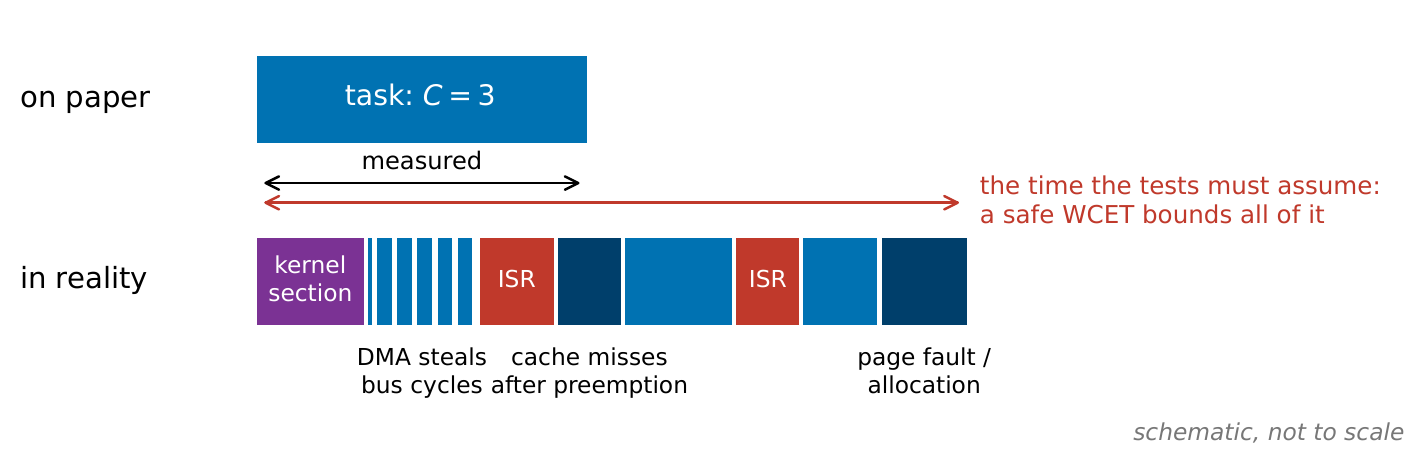
\includegraphics[width=\textwidth]{images/week-06/w6-u3-unpredictability.png}
    \caption{Schematic, not to scale: the same job on paper and on a real system, where a kernel section, interrupts, DMA, cache misses and memory management stretch its execution. The tests are valid only if $C$ is a safe WCET that bounds all of it.}
\end{figure}

\subsection{Where the extra time comes from}
\paragraph{DMA.} The DMA controller and the CPU share the bus to the only memory, so the CPU waits: for a whole block in \textbf{burst} mode, one word at a time in \textbf{cycle stealing}. Dual-port memories exist, but embedded systems must cost a few tens of euros. Fix: a \textbf{time-sliced} bus (fixed slots for CPU and DMA), slower, but the task time no longer depends on the transfers. Really safety-critical designs do without DMA and spend CPU time on the transfers.

\paragraph{Cache.} The hit/miss variance makes the execution time vary, and paging on top makes it worse. The average improves, but the worst case is hard to compute, and each preemption destroys locality and adds misses (one measure on a PowerPC: WCET $+33\%$). Fix: \textbf{disable} or \textbf{lock} the cache, or use a larger, safe WCET. Safety engineers often disable it: every CPU can mark memory as not cacheable (the MPU regions of the scratch-OS have this attribute too), and everything runs at RAM speed, but predictably.

\paragraph{Interrupts.} An interrupt is more important than any scheduler: its ISR preempts any task, and the number of interrupts in a window is hard to bound. Interrupts cannot be disabled, so their impact must be minimised. Fix: a very short ISR that only wakes a \textbf{task} doing the work, with its own priority; or the device treated as \textbf{aperiodic jobs served by a server}, as in this unit. Both are too complex for the scratch-OS and will be studied with FreeRTOS.

\paragraph{System calls.} Tasks that ask the OS for services may block each other, breaking their independence: a non-preemptible kernel section delays even the highest-priority task. System calls cannot be avoided, short of running bare metal (as many avionics applications do). Fix: bound their time and make the kernel \textbf{preemptible}, so that a more important periodic task stops a system call in the middle.

\paragraph{Memory management.} The nightmare of every real-time system: paging and dynamic allocation take a time that depends on the state of memory. Real-time code allocates statically at start-up, without paging, and avoids recursion and unbounded loops. The scratch-OS is perfect from this point of view: no memory management, everything allocated on paper and never changed.

\section{How to solve an exam scheduling exercise}
The last slides collect the rules of the two weeks as guidelines for the exam. The same rules are copied into every exam, so they need not be memorised: practise with them, so as not to lose time at the exam remembering a rule or a formula.

\paragraph{Exam.} One exercise of the first part of the exam is \textbf{always} on scheduling, on one of the algorithms studied: you must know the algorithms and the schedulability conditions, RTA included, and apply them to any exercise. The exam is being redesigned, probably not completely: last year a scheduling exercise was worth about \textbf{4--5 points}, depending on its complexity. It is not difficult, but stress causes confusion: you need a method that works even when your brain shuts down. Two or three exercises can be solved by method alone, about 12 points; with a pass threshold of 14 (not confirmed), only two more points need real thinking. A fast method takes minutes: students with one left after 30 minutes of a one-hour exam. The hyperperiod is small (16, 20 or 25 units, never 100), and the exercises done in class by the end of the semester cover the possible ones.

\subsection{The method}
\begin{enumerate}
    \item \textbf{Read the set}: which algorithm? Periodic tasks ($C$, $T$, $D = T$), one-shot jobs ($a$, $C$, $D$), aperiodic jobs, a server? Note the \textbf{answer keys} asked.
    \item \textbf{Tests first} (\textbf{schedulability first}, before any drawing): $U$, then the test of the algorithm. If $U > 1$, stop, unless the exercise asks for the chart anyway: in the real world too, $U > 1$ is the first problem to solve. RM: the Liu--Layland bound, and RTA if it is inconclusive. EDF: $U \le 1$. Servers: $P$ against the bound, and $U_{s,max}$. One-shot jobs: the absolute deadlines $d = a + D$.
    \item \textbf{Priorities}: write the order once. RM: shorter period first ($1/T$); a server from $T_s$. EDF and Horn: the earliest absolute deadline.
    \item \textbf{Draw slot by slot}, over one hyperperiod or the given horizon: at every release, completion and server period start, \textbf{apply the algorithm} with the conventions listed below. Write the chart and the schedule string, one character per time unit.
    \item \textbf{Read the results} from the chart: finish $f$, $R = f - a$, $L = f - d$, the first miss. They must agree with the tests: for an RM task that meets its deadline, the RTA value is the finish time of its first job.
    \item \textbf{Write the answer file} (\texttt{key=value}, one per line), then check it with \texttt{schedsim}.
\end{enumerate}
\begin{figure}[H]
    \centering
    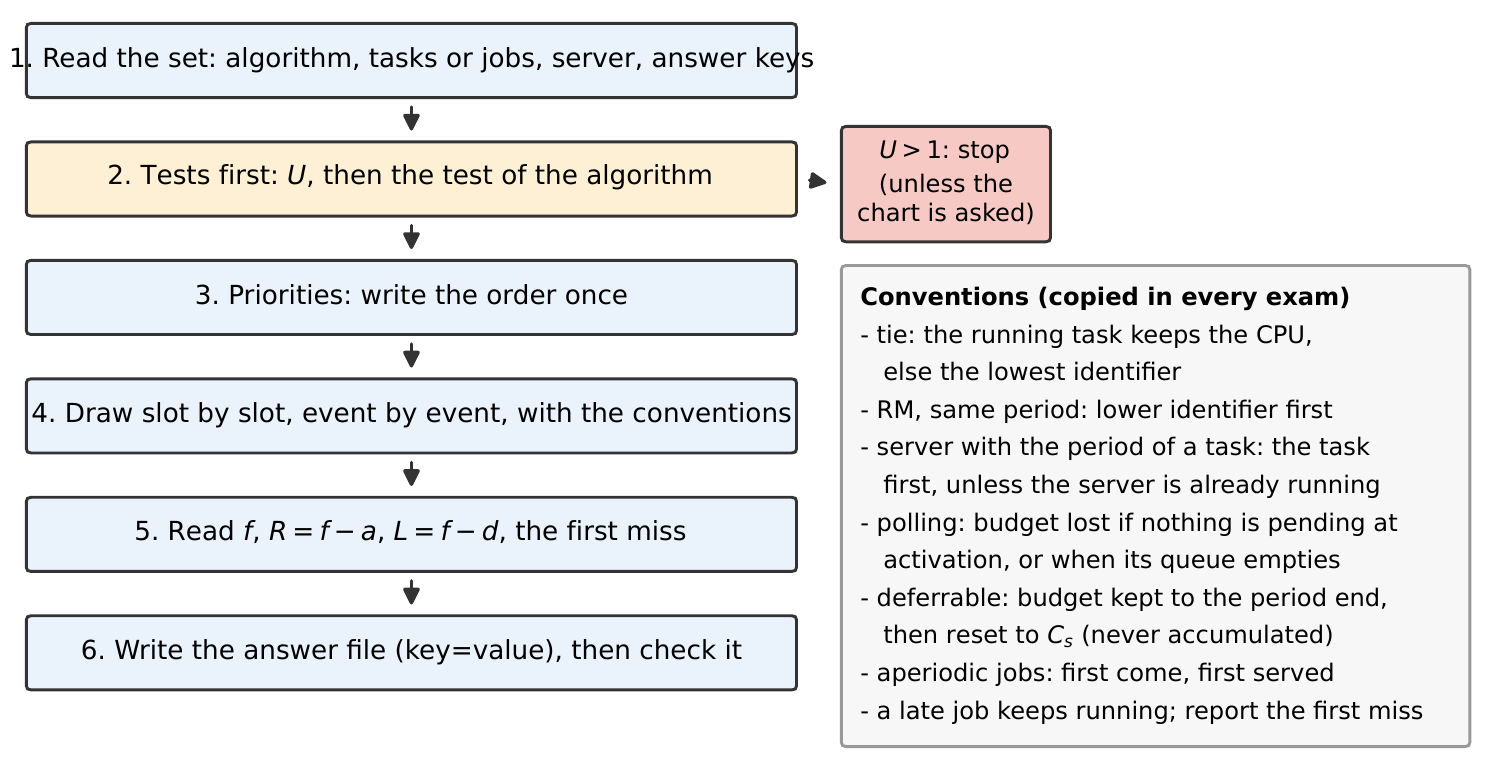
\includegraphics[width=\textwidth]{images/week-06/w6-u3-exam-method.png}
    \caption{The method for an exam scheduling exercise, with the conventions that decide the slots.}
\end{figure}

\subsection{The rules that decide a slot}
The conventions of \texttt{Exam.md} that decide the slots where the choice is not obvious:
\begin{itemize}
    \item \textbf{Tie} in priority or deadline: the running task keeps the CPU. If none of the tied tasks is running, the lowest identifier runs.
    \item \textbf{RM, same period}: the lower identifier has the higher priority.
    \item \textbf{Server}: RM priority from its period $T_s$. With the same period as a task, it loses the tie, as if it had the highest identifier: the task runs first, unless the server is already running.
    \item \textbf{Polling server}: loses its budget when no aperiodic job is pending at its activation ($t = 0, T_s, 2T_s, \dots$), and as soon as its queue becomes empty.
    \item \textbf{Deferrable server}: keeps its budget until the end of its period; at each period start the budget is set back to $C_s$, never accumulated.
    \item \textbf{Aperiodic jobs} (background or server) are served first come, first served.
    \item A job that misses its deadline \textbf{keeps running} until it completes; the first miss is the one reported. In RTA, if $R$ exceeds $D$, $R$ is the first iterate above $D$.
\end{itemize}

\subsection{Practice at home}
\begin{itemize}
    \item \textbf{The week 6 self-assessment} (on Git): exam-style problems with full solutions (one per algorithm of this week, plus mixed problems), each with its task set to \texttt{check}; do as many as you want.
    \item \textbf{The exercise sheet} \texttt{course-material/exercises/scheduling.md}: 22 exercises, two for each algorithm of weeks 5 and 6 (one basic, one harder), with the task files and hidden solutions in \texttt{exercises/scheduling/}.
    \item Solve on paper first, without looking anything up, then \texttt{check}, and read \texttt{explain} only to find your mistake.
    \item \textbf{New exercises} from the tool; the same seed always gives the same exercise, and \texttt{-{}-solution} adds the answer file:
\begin{lstlisting}[language=bash]
    python3 schedsim.py generate <algorithm> --difficulty medium --seed N
\end{lstlisting}
    \item At the exam you have no tool: practise drawing the chart \textbf{by hand}, slot by slot, with the conventions.
\end{itemize}

\subsection*{Self-assessment: how to use it}
The week 6 self-assessment is \textbf{not graded and not submitted}: it only lets you gauge your preparation before the lab. Study first, and read a solution only after committing to an answer. The exercises use the course conventions and answer format; the solutions are the official answers of the tool. To check an answer, save the task set to a file, the answer (\texttt{key=value} lines) to another, and run, from \texttt{course-material/tools/schedsim/}:
\begin{lstlisting}[language=bash]
    python3 schedsim.py check taskset.txt myanswer.txt
\end{lstlisting}
When a question asks only for some keys, add \texttt{-{}-keys} with a comma-separated list, e.g.\ \texttt{-{}-keys U,bound}. The tool marks each line.

\paragraph*{Answer keys for RM.} An RM exercise is answered with \texttt{U}, \texttt{bound} (the Liu--Layland bound, three decimals), one \texttt{R\_<task>} per task, \texttt{feasible} and \texttt{first\_miss}, plus \texttt{schedule} when the chart is asked. Here \texttt{R\_A} is the RTA value of task A: the response time of its first job when the deadline is met, and the first iterate above $D$ when it is missed.

\subsection*{Self-assessment 1: rate monotonic and the Liu--Layland bound}
\begin{lstlisting}
    algorithm: rm
    task A C=1 T=4
    task B C=1 T=6
    task C C=2 T=12
\end{lstlisting}
\begin{enumerate}
    \item Which rule gives the priorities in RM? Is a priority fixed, or does it change at run time?
    \item Compute $U$ and the Liu--Layland bound. What does the test tell you?
    \item Give the RM schedule over one hyperperiod and the response times.
\end{enumerate}

\textbf{Solution.}
\begin{enumerate}
    \item The task with the shortest period has the highest priority; the priority is fixed, decided once from $T$.
    \item
    \[
    U = \frac{1}{4} + \frac{1}{6} + \frac{2}{12} = \frac{3}{12} + \frac{2}{12} + \frac{2}{12} = \frac{7}{12} = 0.583, \qquad U_{lub}(3) = 3 \left( 2^{1/3} - 1 \right) = 0.780
    \]
    $0.583 \le 0.780$: the test passes: feasible with RM, no further analysis needed.
    \item $H = \mathrm{LCM}(4, 6, 12) = 12$. A ($T = 4$) runs first, then B ($T = 6$), then C ($T = 12$), which runs 2--4; all deadlines are met, as the test said.
\begin{verbatim}
    time  0         10
        |.........|..
    A     #...#...#...
    B     .#....#.....
    C     ..##........
    CPU   ABCCA.B.A...
\end{verbatim}
\begin{verbatim}
    schedule=ABCCA.B.A...
    U=0.583
    bound=0.780
    R_A=1
    R_B=2
    R_C=4
    feasible=yes
    first_miss=none
\end{verbatim}
\end{enumerate}

\subsection*{Self-assessment 2: the bound is sufficient, not necessary}
\begin{lstlisting}
    algorithm: rm
    task A C=1 T=2
    task B C=1 T=4
    task C C=2 T=8
\end{lstlisting}
Compute $U$ and the bound and apply the test. Then use RTA to decide whether the set is feasible with RM. What does this tell you about the Liu--Layland test? Give \texttt{U}, \texttt{bound}, \texttt{R\_A}, \texttt{R\_B}, \texttt{R\_C} and \texttt{feasible}.

\textbf{Solution.}
\[
U = \frac{1}{2} + \frac{1}{4} + \frac{2}{8} = 1, \qquad U_{lub}(3) = 0.780
\]
$U > U_{lub}(3)$: the test is inconclusive (it does not say ``not feasible''). RTA, highest priority first (A: $T = 2$, B: $T = 4$, C: $T = 8$):
\begin{itemize}
    \item $R_A = C_A = 1$;
    \item B: $R = 1 + \lceil R/2 \rceil \cdot 1$, iterates $1 \to 2 \to 2$: $R_B = 2$;
    \item C: $R = 2 + \lceil R/2 \rceil \cdot 1 + \lceil R/4 \rceil \cdot 1$, iterates $2 \to 4 \to 5 \to 7 \to 8 \to 8$: $R_C = 8 \le 8$.
\end{itemize}
\begin{verbatim}
    time  0       8
        |.......|
    A     #.#.#.#.
    B     .#...#..
    C     ...#...#
    CPU   ABACABAC
\end{verbatim}
\begin{verbatim}
    U=1
    bound=0.780
    R_A=1
    R_B=2
    R_C=8
    feasible=yes
\end{verbatim}
Feasible even with $U = 1$: the bound is only sufficient, a guarantee for the worst case over all possible periods. Here the periods are \textbf{harmonic} (each divides the next), and with harmonic periods RM can use 100\% of the CPU. Above the bound, only RTA (exact for RM) decides.

\subsection*{Self-assessment 3: response-time analysis}
\begin{lstlisting}
    algorithm: rm
    task A C=2 T=6
    task B C=3 T=9
    task C C=4 T=18
\end{lstlisting}
Apply the RM test and, if needed, RTA. Show every iteration for C.

\textbf{Solution.}
\[
U = \frac{2}{6} + \frac{3}{9} + \frac{4}{18} = \frac{6}{18} + \frac{6}{18} + \frac{4}{18} = \frac{16}{18} = 0.889 > 0.780
\]
The test is inconclusive. RTA, with $R = C + \sum \lceil R / T_j \rceil C_j$ over the tasks with a shorter period:
\begin{itemize}
    \item $R_A = 2$;
    \item B: $3 + \lceil R/6 \rceil \cdot 2$, iterates $3 \to 5 \to 5$: $R_B = 5$;
    \item C: $4 + \lceil R/6 \rceil \cdot 2 + \lceil R/9 \rceil \cdot 3$:
\end{itemize}
\[
\begin{aligned}
R_C^{(0)} &= 4 \\
R_C^{(1)} &= 4 + \left\lceil \tfrac{4}{6} \right\rceil \cdot 2 + \left\lceil \tfrac{4}{9} \right\rceil \cdot 3 = 4 + 2 + 3 = 9 \\
R_C^{(2)} &= 4 + \left\lceil \tfrac{9}{6} \right\rceil \cdot 2 + \left\lceil \tfrac{9}{9} \right\rceil \cdot 3 = 4 + 4 + 3 = 11 \\
R_C^{(3)} &= 4 + \left\lceil \tfrac{11}{6} \right\rceil \cdot 2 + \left\lceil \tfrac{11}{9} \right\rceil \cdot 3 = 4 + 4 + 6 = 14 \\
R_C^{(4)} &= 4 + \left\lceil \tfrac{14}{6} \right\rceil \cdot 2 + \left\lceil \tfrac{14}{9} \right\rceil \cdot 3 = 4 + 6 + 6 = 16 \\
R_C^{(5)} &= 4 + \left\lceil \tfrac{16}{6} \right\rceil \cdot 2 + \left\lceil \tfrac{16}{9} \right\rceil \cdot 3 = 4 + 6 + 6 = 16
\end{aligned}
\]
Fixed point, $R_C = 16 \le 18$. $H = \mathrm{LCM}(6, 9, 18) = 18$:
\begin{verbatim}
    time  0         10
        |.........|.......
    A     ##....##....##....
    B     ..###....###......
    C     .....#..#.....##..
    CPU   AABBBCAACBBBAACC..
\end{verbatim}
\begin{verbatim}
    schedule=AABBBCAACBBBAACC..
    U=0.889
    bound=0.780
    R_A=2
    R_B=5
    R_C=16
    feasible=yes
    first_miss=none
\end{verbatim}
Feasible with RM, although above the bound.

\subsection*{Self-assessment 4: RM fails, EDF succeeds}
\begin{lstlisting}
    algorithm: rm
    task A C=3 T=8
    task B C=3 T=5
\end{lstlisting}
\begin{enumerate}
    \item Is this set feasible with RM? Give the full answer.
    \item Is it feasible with EDF? Give the full answer.
    \item What is the EDF feasibility condition for periodic tasks with $D = T$, and why can EDF succeed where RM fails?
\end{enumerate}

\textbf{Solution.}
\begin{enumerate}
    \item B has the shorter period (5), so it has the higher priority (the identifier does not matter).
    \[
    U = \frac{3}{8} + \frac{3}{5} = \frac{15}{40} + \frac{24}{40} = \frac{39}{40} = 0.975 > 0.828
    \]
    Inconclusive. RTA: $R_B = 3$. A: $3 + \lceil R/5 \rceil \cdot 3$, iterates $3 \to 6 \to 9$: the first iterate above $D = 8$ is 9, so \textbf{A misses its deadline}, first at 8. $H = \mathrm{LCM}(8, 5) = 40$:

    \begin{verbatim}
    time  0         10        20        30        40
        |.........|.........|.........|.........|
    A     ...##...##...##...##...##...##...##...#.   <- A1 misses its deadline at 8
    B     ###..###..###..###..###..###..###..###..
    CPU   BBBAABBBAABBBAABBBAABBBAABBBAABBBAABBBA.
\end{verbatim}
\begin{verbatim}
    schedule=BBBAABBBAABBBAABBBAABBBAABBBAABBBAABBBA.
    U=0.975
    bound=0.828
    R_A=9
    R_B=3
    feasible=no
    first_miss=A@8
\end{verbatim}
    \item With EDF, on the same set:
\begin{verbatim}
    time  0         10        20        30        40
        |.........|.........|.........|.........|
    A     ...###...#...##...###...#...##...###....
    B     ###...###.###..###...###.###..###...###.
    CPU   BBBAAABBBABBBAABBBAAABBBABBBAABBBAAABBB.
\end{verbatim}
\begin{verbatim}
    schedule=BBBAAABBBABBBAABBBAAABBBABBBAABBBAAABBB.
    U=0.975
    feasible=yes
    first_miss=none
\end{verbatim}
    \item EDF is feasible if and only if $U \le 1$: $U = 0.975$, feasible. With priorities computed at run time (earliest absolute deadline), EDF reorders the jobs and uses the whole CPU; the fixed priorities of RM give a lower guaranteed limit.
\end{enumerate}

\subsection*{Self-assessment 5: overload}
The same set, once with EDF and once with RM:
\begin{lstlisting}
    algorithm: edf
    task A C=2 T=5
    task B C=3 T=6
    task C C=2 T=10
\end{lstlisting}

\begin{enumerate}
    \item Give \texttt{U}, \texttt{feasible} and \texttt{first\_miss} under EDF.
    \item Give \texttt{U}, the response times, \texttt{feasible} and \texttt{first\_miss} under RM.
    \item With the RM result, which task is hurt? Why is this ``graceful'' for RM, and why is it hard to say in advance which task misses under EDF?
\end{enumerate}

\textbf{Solution.}
\begin{enumerate}
    \item \[
    U = \frac{2}{5} + \frac{3}{6} + \frac{2}{10} = \frac{12}{30} + \frac{15}{30} + \frac{6}{30} = \frac{33}{30} = 1.100 > 1
    \]
    No scheduler can meet every deadline.
\begin{verbatim}
    U=1.100
    feasible=no
    first_miss=C@20
\end{verbatim}
    \item RTA with A ($T = 5$) $>$ B ($T = 6$) $>$ C ($T = 10$): $R_A = 2$; $R_B = 3 + \lceil 3/5 \rceil \cdot 2 = 5$, a fixed point. C: $2 + \lceil R/5 \rceil \cdot 2 + \lceil R/6 \rceil \cdot 3$, iterates $2 \to 7 \to 12$: the first iterate above $D = 10$ is 12, so C misses at 10.
\begin{verbatim}
    U=1.100
    R_A=2
    R_B=5
    R_C=12
    feasible=no
    first_miss=C@10
\end{verbatim}
    \item Under RM only C, the \textbf{lowest-priority} task, is hurt; A and B keep their deadlines: fixed priorities keep the damage on the least important task, a \textbf{graceful} degradation. Under EDF a job's priority depends on its current deadline, so the first task to miss (C at 20 here) is not tied to any fixed importance, and is hard to predict.
\end{enumerate}

\subsection*{Self-assessment 6: the notation $\alpha \,|\, \beta \,|\, \gamma$}
\begin{enumerate}
    \item Explain the three fields of $\alpha \,|\, \beta \,|\, \gamma$.
    \item Decode $1 \,|\, \textit{sync} \,|\, L_{max}$ and $1 \,|\, \textit{preem} \,|\, L_{max}$. Which algorithm solves each?
    \item What does $L_{max} \le 0$ mean?
\end{enumerate}

\textbf{Solution.}
\begin{enumerate}
    \item $\alpha$: the machine (\texttt{1} = one CPU). $\beta$: the task and resource characteristics (\texttt{preem} = preemption allowed, \texttt{sync} = all jobs arrive at the same time, empty = arbitrary arrival times). $\gamma$: the goal to minimise (here $L_{max}$, the maximum lateness).
    \item $1 \,|\, \textit{sync} \,|\, L_{max}$: one CPU, all jobs at 0, minimise $L_{max}$: \textbf{Jackson's algorithm (EDD)}. $1 \,|\, \textit{preem} \,|\, L_{max}$: preemption allowed, arbitrary arrivals: \textbf{Horn's algorithm} (preemptive EDF).
    \item The lateness is $L = f - d$ (finish time minus absolute deadline): $L_{max} \le 0$ means that \textbf{every job finishes by its deadline}.
\end{enumerate}

\subsection*{Self-assessment 7: Jackson's algorithm (EDD)}
All jobs arrive at time 0. Compute the EDD schedule, the latenesses, $L_{max}$, \texttt{feasible} and \texttt{first\_miss}. Then explain why no other non-preemptive order can have a smaller $L_{max}$.
\begin{lstlisting}
    algorithm: jackson
    job A a=0 C=3 D=7
    job B a=0 C=2 D=5
    job C a=0 C=4 D=9
    job D a=0 C=1 D=3
    job E a=0 C=3 D=14
\end{lstlisting}

\textbf{Solution.} Order by non-decreasing deadline: D (3), B (5), A (7), C (9), E (14). The finish times are 1, 3, 6, 10, 13, so $L_C = 10 - 9 = 1$ is the only positive lateness.
\begin{verbatim}
    time  0         10
        |.........|...
    A     ...###.......
    B     .##..........
    C     ......####...   <- C misses its deadline at 9
    D     #............
    E     ..........###
    CPU   DBBAAACCCCEEE
\end{verbatim}
\begin{verbatim}
    schedule=DBBAAACCCCEEE
    L_A=-1
    L_B=-2
    L_C=1
    L_D=-2
    L_E=-1
    Lmax=1
    feasible=no
    first_miss=C@9
\end{verbatim}
\paragraph*{Why EDD is optimal (exchange argument).} Swapping a job X with a later deadline that runs right before a job Y with an earlier one never increases $L_{max}$: Y finishes earlier, and X finishes where Y used to, with a later deadline. Repeated swaps turn any order into EDD without increasing $L_{max}$, so EDD is optimal: here $L_{max} = 1$ is the best possible, and no reordering makes the set feasible.

\subsection*{Self-assessment 8: Horn's algorithm}
The jobs arrive at different times and may be preempted. Compute the schedule, the latenesses, $L_{max}$, \texttt{feasible} and \texttt{first\_miss}. At time 3, why does C preempt B?
\begin{lstlisting}
    algorithm: horn
    job A a=0 C=5 D=12
    job B a=2 C=3 D=6
    job C a=3 C=1 D=4
    job D a=6 C=2 D=5
\end{lstlisting}

\textbf{Solution.} Absolute deadlines: A 12, B $2 + 6 = 8$, C $3 + 4 = 7$, D $6 + 5 = 11$. A runs alone 0--2; at 2, B ($d = 8$) preempts A; at 3, C ($d = 7$) has a \textbf{strictly earlier} deadline than B ($d = 8$), so it preempts B. B resumes at 4 and ends at 6; D ($d = 11$) runs before A ($d = 12$), which ends last, at 11.
\begin{verbatim}
    time  0         10
        |.........|
    A     ##......###
    B     ..#.##.....
    C     ...#.......
    D     ......##...
    CPU   AABCBBDDAAA
\end{verbatim}
\begin{verbatim}
    schedule=AABCBBDDAAA
    L_A=-1
    L_B=-2
    L_C=-3
    L_D=-3
    Lmax=-1
    feasible=yes
    first_miss=none
\end{verbatim}
All latenesses are negative: the set is feasible.

\subsection*{Self-assessment 9: background service}
The periodic tasks use RM; the aperiodic jobs a and b run in background. Compute the schedule, $U$, the bound, the response times of the periodic tasks and of the aperiodic jobs, \texttt{feasible} and \texttt{first\_miss}. What is the main weakness of background service?
\begin{lstlisting}
    algorithm: background
    task A C=2 T=6
    task B C=3 T=9
    aperiodic a a=1 C=2
    aperiodic b a=7 C=1
\end{lstlisting}

\textbf{Solution.} The aperiodic jobs run only when \textbf{no periodic job is ready}. a arrives at 1, but A and B keep the CPU until 5: a starts at 5, is preempted by A at 6, and ends at 9, $R_a = 9 - 1 = 8$. b arrives at 7 and waits until the periodic work ends at 14: it ends at 15, $R_b = 15 - 7 = 8$.
\begin{verbatim}
    time  0         10
        |.........|.......
    A     ##....##....##....
    B     ..###....###......
    a     .....#..#.........
    b     ..............#...
    CPU   AABBBaAAaBBBAAb...
\end{verbatim}
\begin{verbatim}
    schedule=AABBBaAAaBBBAAb...
    U=0.667
    bound=0.828
    R_A=2
    R_B=5
    R_a=8
    R_b=8
    feasible=yes
    first_miss=none
\end{verbatim}
The periodic tasks are not disturbed ($R_A$ and $R_B$ are those of plain RM). The weakness: the aperiodic response time is \textbf{long and depends on the periodic load}, very long with a high $U$.

\subsection*{Self-assessment 10: polling server and lost budget}
The periodic tasks use RM with a polling server ($C_s = 2$, $T_s = 6$). A server with the same period as a task has the same RM priority, and the task runs first. Compute the schedule (horizon 18) and the response times of a and b. Then explain why a had to wait until time 8, although it arrived at time 1.
\begin{lstlisting}
    algorithm: polling
    horizon: 18
    task A C=2 T=6
    task B C=3 T=12
    server polling Cs=2 Ts=6
    aperiodic a a=1 C=1
    aperiodic b a=7 C=2
\end{lstlisting}

\textbf{Solution.} At $t = 0$ \textbf{no aperiodic job is pending}, so the budget is lost until $t = 6$: a (arrival 1) cannot be served in that period. At 6 the budget is 2 and a is pending, but A, with the same period, wins the tie: A runs 6--8, then the server serves a at 8 (budget $2 \to 1$) and b (arrival 7) at 9 (budget $1 \to 0$); the second slot of b waits for the next period: A runs 12--14, and b ends at 15.
\begin{verbatim}
    time  0         10
        |.........|.......
    A     ##....##....##....
    B     ..###..........###
    a     ........#.........
    b     .........#....#...
    CPU   AABBB.AAab..AAbBBB
\end{verbatim}
\begin{verbatim}
    schedule=AABBB.AAab..AAbBBB
    U=0.583
    Us=0.333
    P=1.667
    bound=1.500
    Usmax=0.200
    R_a=8
    R_b=8
    feasible=yes
    first_miss=none
\end{verbatim}
b arrives \textbf{during} the period 6--12 and is served in it, because the budget is still there (a was pending at the activation at 6, and the queue had not emptied). a arrived in the period 0--6 after the budget was lost at 0: the polling server looks at the queue only at its activation and when the queue becomes empty.

\subsection*{Self-assessment 11: deferrable server and the back-to-back effect}
The same task set, now with a deferrable server ($C_s = 2$, $T_s = 6$). Compute the schedule (horizon 18) and the response times, and compare them with Self-assessment 10. Then explain the \textbf{back-to-back} effect, and why it makes the feasibility test of the deferrable server stricter.
\begin{lstlisting}
    algorithm: deferrable
    horizon: 18
    task A C=2 T=6
    task B C=3 T=12
    server deferrable Cs=2 Ts=6
    aperiodic a a=1 C=1
    aperiodic b a=7 C=2
\end{lstlisting}

\textbf{Solution.} The deferrable server \textbf{keeps its budget} until the end of its period, so a (arrival 1) is served as soon as the higher-priority work is done, at 2 (budget $2 \to 1$). At 6 the budget is set back to 2 (not 3: it never accumulates); b (arrival 7) is served 8--10, after A.
\begin{verbatim}
    time  0         10
        |.........|.......
    A     ##....##....##....
    B     ...###........###.
    a     ..#...............
    b     ........##........
    CPU   AAaBBBAAbb..AABBB.
\end{verbatim}
\begin{verbatim}
    schedule=AAaBBBAAbb..AABBB.
    U=0.583
    Us=0.333
    P=1.667
    bound=1.400
    Usmax=0.143
    R_a=2
    R_b=3
    feasible=yes
    first_miss=none
\end{verbatim}
The response times drop from 8 and 8 to 2 and 3. The price is the \textbf{back-to-back effect}: budget used at the end of a period, then a full budget at the start of the next; with $C_s = 2$, $T_s = 6$ the server can run 4--6 and then 6--8, $2C_s$ in a row, which a periodic task never does. Lower-priority tasks can suffer more interference than from a plain periodic task with $C_s$ and $T_s$, hence the smaller bound $(U_s + 2)/(2U_s + 1)$ instead of $2/(U_s + 1)$.

\subsection*{Self-assessment 12: polling server, test and sizing}
The periodic tasks A and B use RM with a polling server $C_s = 2$, $T_s = 6$. Compute $U$, $U_s$, $P = \prod (U_i + 1)$, the polling bound $2/(U_s + 1)$ and $U_{s,max}$. Does the server pass the test? What is the largest integer $C_s$ when $T_s$ is the shortest period? Then apply Liu--Layland with the server as a third periodic task: does it pass, and which test leaves more room for the server?
\begin{lstlisting}
    algorithm: polling
    task A C=1 T=6
    task B C=2 T=9
    server polling Cs=2 Ts=6
\end{lstlisting}

\textbf{Solution.}
\[
U = \frac{1}{6} + \frac{2}{9} = 0.389, \quad U_s = \frac{2}{6} = 0.333, \quad P = \left( \frac{1}{6} + 1 \right) \left( \frac{2}{9} + 1 \right) = 1.426, \quad \text{bound} = \frac{2}{0.333 + 1} = 1.500
\]
$P = 1.426 \le 1.500$: the test \textbf{passes} (it is a sufficient test), so the set is feasible with RM. $U_{s,max} = (2 - P)/P = 0.403$.
\begin{verbatim}
    U=0.389
    Us=0.333
    P=1.426
    bound=1.500
    Usmax=0.403
\end{verbatim}
With $T_s = 6$: $C_s \le 0.403 \cdot 6 = 2.42$, so the largest integer is $C_s = 2$: the given server is exactly the largest one.

Liu--Layland with 3 tasks: bound $3 (2^{1/3} - 1) = 0.780$, and $U + U_s = 0.389 + 0.333 = 0.722 \le 0.780$: it passes too, but leaves the server only $0.780 - 0.389 = 0.391$, below the $0.403$ of the product test, which never accepts less and often more.

\subsection*{Self-assessment 13: deferrable server, test and sizing}
The same periodic tasks, now with a deferrable server $C_s = 2$, $T_s = 6$. Compute $U$, $U_s$, $P$, the deferrable bound $(U_s + 2)/(2U_s + 1)$ and $U_{s,max} = (2 - P)/(2P - 1)$ (show how it follows from the bound). What can you say about the server? What is the largest integer $C_s$ with $T_s = 6$?
\begin{lstlisting}
    algorithm: deferrable
    task A C=1 T=6
    task B C=2 T=9
    server deferrable Cs=2 Ts=6
\end{lstlisting}

\textbf{Solution.} $P = 1.426$ as before; bound $= (0.333 + 2)/(2 \cdot 0.333 + 1) = 1.400$. $P = 1.426 > 1.400$: the test is inconclusive (it is only sufficient: it does not prove that the set is not feasible). Setting the two sides equal:
\[
P = \frac{U_s + 2}{2U_s + 1} \;\Rightarrow\; P(2U_s + 1) = U_s + 2 \;\Rightarrow\; U_s(2P - 1) = 2 - P \;\Rightarrow\; U_{s,max} = \frac{2 - P}{2P - 1} = \frac{0.574}{1.852} = 0.310
\]
\begin{verbatim}
    U=0.389
    Us=0.333
    P=1.426
    bound=1.400
    Usmax=0.310
\end{verbatim}
$C_s \le 0.310 \cdot 6 = 1.86$: the largest integer is $C_s = 1$. The server that passes as polling (Self-assessment 12) fails as deferrable: faster answers need a smaller budget to be guaranteed.

\subsection*{Self-assessment 14: sources of unpredictability}
A task has a measured execution time of 3\,ms. Name four sources that can make its WCET larger and hard to bound, say how each one acts, and say why this matters for the tests of this week.

\textbf{Solution.}
\begin{itemize}
    \item \textbf{DMA}: it steals bus cycles from the CPU, delaying memory accesses by an amount that depends on other devices.
    \item \textbf{Cache}: hit and miss times differ a lot, and the hit/miss pattern depends on the history of the other tasks.
    \item \textbf{Interrupts}: they can preempt the task at any time, for a time that is hard to bound.
    \item \textbf{System calls}: non-preemptive kernel sections can block a high-priority task behind the kernel call of a lower one.
    \item \textbf{Memory management}: paging and dynamic allocation add long, variable delays (a page fault, a search for a free block).
\end{itemize}
All the tests (bound, RTA, EDF, servers) take $C$ as a \textbf{known upper bound}. If $C$ is not a safe WCET, the tests prove nothing: a hard real-time system therefore avoids or bounds these mechanisms.

\subsection*{Exam practice}
The next problems are mixed, like those of the exam, on the algorithms of all three units. Solve them on paper first, slot by slot, with the conventions, then check them with the tool. Self-assessments 18 to 22 also have their task-set and answer files in \texttt{course-material/exercises/scheduling/}.

\subsection*{Self-assessment 15: periodic set, bound, RTA, RM and EDF}
\begin{enumerate}
    \item Apply the Liu--Layland test.
    \item If it is inconclusive, apply RTA.
    \item Give the RM answer.
    \item Is the set feasible with EDF? Give the full answer for EDF too.
\end{enumerate}
\begin{lstlisting}
    algorithm: rm
    task A C=2 T=5
    task B C=2 T=10
    task C C=3 T=15
\end{lstlisting}

\textbf{Solution.}
\begin{enumerate}
    \item $U = 2/5 + 2/10 + 3/15 = 0.800 > 0.780$: inconclusive.
    \item RTA: $R_A = 2$. B: $2 + \lceil R/5 \rceil \cdot 2$, iterates $2 \to 4 \to 4$: $R_B = 4$. C: $3 + \lceil R/5 \rceil \cdot 2 + \lceil R/10 \rceil \cdot 2$, iterates $3 \to 7 \to 9 \to 9$: $R_C = 9 \le 15$.
    \item RM, all deadlines met; $H = \mathrm{LCM}(5, 10, 15) = 30$:
\begin{verbatim}
    time  0         10        20        30
        |.........|.........|.........|
    A     ##...##...##...##...##...##...
    B     ..##........##........##......
    C     ....#..##........###..........
    CPU   AABBCAACC.AABB.AACCCAABB.AA...
\end{verbatim}

\begin{verbatim}
    schedule=AABBCAACC.AABB.AACCCAABB.AA...
    U=0.800
    bound=0.780
    R_A=2
    R_B=4
    R_C=9
    feasible=yes
    first_miss=none
\end{verbatim}
    \item The same tasks with EDF (\texttt{algorithm: edf}): $U = 0.8 \le 1$, so EDF is feasible. Here the EDF schedule is the same as the RM one:
\begin{verbatim}
    schedule=AABBCAACC.AABB.AACCCAABB.AA...
    U=0.800
    feasible=yes
    first_miss=none
\end{verbatim}
\end{enumerate}

\subsection*{Self-assessment 16: mixed set with a deferrable server}
The periodic tasks A and B use RM; the deferrable server has $C_s = 1$, $T_s = 4$.
\begin{enumerate}
    \item Compute the server test and $U_{s,max}$.
    \item Compute the schedule (hyperperiod 20) and the response times of a, b and c.
    \item Does the test prove that the set is feasible? Is the set feasible anyway?
\end{enumerate}
\begin{lstlisting}
    algorithm: deferrable
    task A C=1 T=4
    task B C=3 T=10
    server deferrable Cs=1 Ts=4
    aperiodic a a=3 C=2
    aperiodic b a=9 C=1
    aperiodic c a=10 C=1
\end{lstlisting}

\textbf{Solution.}
\begin{enumerate}
    \item $U = 1/4 + 3/10 = 0.550$, $U_s = 1/4 = 0.250$, $P = (1/4 + 1)(3/10 + 1) = 1.625$, bound $= 2.25/1.5 = 1.500$. $P > \text{bound}$: inconclusive. $U_{s,max} = 0.375/2.25 = 0.167$; with $T_s = 4$, $C_s \le 0.67$: no integer $C_s \ge 1$ passes the test with this period.
    \item Job a (arrival 3) uses the budget at 3 and, after the replenishment at 4, again at 4: at 4 the server is the running entity (a is not finished), so on the tie with A it keeps the CPU; $R_a = 5 - 3 = 2$. Job b (arrival 9) uses the budget at 9: $R_b = 1$. Job c (arrival 10) finds the budget empty (replenished only at 12); at 12 the server is not running and loses the tie with A, so A runs at 12 and c at 13: $R_c = 14 - 10 = 4$.
\begin{verbatim}
    time  0         10        20
        |.........|.........|
    A     #....#..#...#...#...
    B     .##...#...##..#.....
    a     ...##...............
    b     .........#..........
    c     .............#......
    CPU   ABBaaAB.AbBBAcB.A...
\end{verbatim}
\begin{verbatim}
    schedule=ABBaaAB.AbBBAcB.A...
    U=0.550
    Us=0.250
    P=1.625
    bound=1.500
    Usmax=0.167
    R_a=2
    R_b=1
    R_c=4
    feasible=yes
    first_miss=none
\end{verbatim}
    \item The test does not prove feasibility, being only sufficient. This run shows no miss, but in real life the arrival times of the aperiodic jobs are not known in advance.
\end{enumerate}

\subsection*{Self-assessment 17: Horn with a missed deadline}
\begin{enumerate}
    \item Compute the Horn schedule, the latenesses and $L_{max}$.
    \item Which job is late, and by how much?
    \item Would a non-preemptive order help? Why or why not?
\end{enumerate}
\begin{lstlisting}
    algorithm: horn
    job A a=0 C=4 D=7
    job B a=1 C=3 D=5
    job C a=2 C=2 D=3
    job D a=5 C=2 D=6
\end{lstlisting}

\textbf{Solution.}
\begin{enumerate}
    \item Absolute deadlines: A 7, B $1 + 5 = 6$, C $2 + 3 = 5$, D $5 + 6 = 11$. A runs 0--1; B preempts it at 1 ($6 < 7$); C preempts B at 2 ($5 < 6$) and ends at 4; B runs 4--6 (D arrives at 5 with $d = 11$: no preemption); A runs 6--9; D runs 9--11.
\begin{verbatim}
    time  0         10
        |.........|
    A     #.....###..   <- A misses its deadline at 7
    B     .#..##.....
    C     ..##.......
    D     .........##
    CPU   ABCCBBAAADD
\end{verbatim}
\begin{verbatim}
    schedule=ABCCBBAAADD
    L_A=2
    L_B=0
    L_C=-1
    L_D=0
    Lmax=2
    feasible=no
    first_miss=A@7
\end{verbatim}
    \item \textbf{A} is late: it ends at 9 for a deadline of 7, so $L_A = 2 = L_{max}$. The first miss is at 7.
    \item No: Horn's algorithm minimises $L_{max}$ among all the schedules of $1 \,|\, \textit{preem} \,|\, L_{max}$, non-preemptive ones included. $L_{max} = 2$ is the best possible: on one CPU the set cannot meet all its deadlines, whatever the order.
\end{enumerate}

\subsection*{Self-assessment 18: rate monotonic above the bound}
Three periodic tasks, phase 0, $D = T$, scheduled with RM (file \texttt{exercises/scheduling/w6-u3-p1.txt}).
\begin{enumerate}
    \item Compute $U$ and the Liu--Layland bound. What does the bound test tell you?
    \item Compute the response time of every task with RTA. Is the set feasible?
    \item Draw the schedule over the hyperperiod and write the schedule string.
    \item On the chart, when does the first job of C finish? Compare it with $R_C$.
\end{enumerate}
\begin{lstlisting}
    algorithm: rm
    task A C=1 T=3
    task B C=2 T=8
    task C C=3 T=12
\end{lstlisting}

\textbf{Solution.}
\begin{enumerate}
    \item $U = 1/3 + 2/8 + 3/12 = 10/12 = 5/6 = 0.833$; $U_{lub}(3) = 3 (2^{1/3} - 1) = 0.780$. $0.833 > 0.780$: inconclusive, use RTA.
    \item Priorities (shorter period first): A $>$ B $>$ C.
\begin{verbatim}
    A: no interference                                       R_A = 1 <= 3
    B: R(0) = 2, R(1) = 2 + ceil(2/3)*1 = 3, R(2) = 3         R_B = 3 <= 8
    C: R(0) = 3
       R(1) = 3 + ceil(3/3)*1 + ceil(3/8)*2 = 6
       R(2) = 3 + ceil(6/3)*1 + ceil(6/8)*2 = 7
       R(3) = 3 + ceil(7/3)*1 + ceil(7/8)*2 = 8
       R(4) = 3 + ceil(8/3)*1 + ceil(8/8)*2 = 8  fixed point  R_C = 8 <= 12
\end{verbatim}
    Every $R \le D$: feasible. The bound failed, but the set is feasible: the Liu--Layland test is sufficient, not necessary.
    \item $H = \mathrm{LCM}(3, 8, 12) = 24$:
\begin{verbatim}
    time  0         10        20
        |.........|.........|...
    A     #..#..#..#..#..#..#..#..
    B     .##.....#.#.....##......
    C     ....##.#.....##....#....
    CPU   ABBACCACBAB.ACCABBAC.A..
\end{verbatim}
\begin{verbatim}
    schedule=ABBACCACBAB.ACCABBAC.A..
    U=5/6
    bound=0.780
    R_A=1
    R_B=3
    R_C=8
    feasible=yes
    first_miss=none
\end{verbatim}
    \texttt{U=5/6}: a fraction is accepted by the tool.
    \item $C_1$ runs in slots 4, 5 and 7 and finishes at \textbf{8} $= R_C$: all the tasks start together at 0 (the critical instant), so the first job of C has the worst response time. $C_2$ (released at 12) finishes at 20: $R = 8$ again, never more.
\end{enumerate}

\subsection*{Self-assessment 19: RM or EDF, and the ties}
Three periodic tasks, phase 0, $D = T$ (files \texttt{exercises/scheduling/w6-u3-p2-rm.txt} and, for EDF, the same tasks with \texttt{algorithm: edf}, \texttt{w6-u3-p2-edf.txt}).
\begin{enumerate}
    \item Compute $U$. Can some algorithm meet every deadline? What does the Liu--Layland bound say?
    \item Run RTA for RM. Is the set feasible with RM? If not, give the first miss.
    \item Draw the RM schedule over the hyperperiod.
    \item Draw the EDF schedule over the hyperperiod. At $t = 6, 15, 16, 17$ two or more jobs have the same absolute deadline: which one runs, and by which rule?
\end{enumerate}
\begin{lstlisting}
    algorithm: rm
    task A C=2 T=4
    task B C=1 T=5
    task C C=3 T=10
\end{lstlisting}

\textbf{Solution.}
\begin{enumerate}
    \item $U = 2/4 + 1/5 + 3/10 = 20/20 = 1$. $U \le 1$: EDF meets every deadline (the EDF test is exact). $U_{lub}(3) = 0.780 < 1$: inconclusive for RM, use RTA.
    \item Priorities: A $>$ B $>$ C.
\begin{verbatim}
    A: no interference                                       R_A = 2 <= 4
    B: R(0) = 1, R(1) = 1 + ceil(1/4)*2 = 3, R(2) = 3         R_B = 3 <= 5
    C: R(0) = 3
       R(1) = 3 + ceil(3/4)*2 + ceil(3/5)*1 = 6
       R(2) = 3 + ceil(6/4)*2 + ceil(6/5)*1 = 9
       R(3) = 3 + ceil(9/4)*2 + ceil(9/5)*1 = 11 > 10: stop   R_C = 11 > D = 10
\end{verbatim}
    RM is not feasible, \texttt{first\_miss=C@10}; $R_C = 11$ is the first iterate above $D$ (the convention), not the real finish time of $C_1$, which is 12.
    \item RM, $H = \mathrm{LCM}(4, 5, 10) = 20$:
\begin{verbatim}
    time  0         10        20
        |.........|.........|
    A     ##..##..##..##..##..
    B     ..#...#...#....#....
    C     ...#...#...#..#...##   <- C1 misses its deadline at 10
    CPU   AABCAABCAABCAACBAACC
\end{verbatim}

\begin{verbatim}
    schedule=AABCAABCAABCAACBAACC
    U=1
    bound=0.780
    R_A=2
    R_B=3
    R_C=11
    feasible=no
    first_miss=C@10
\end{verbatim}

    A and B leave C one slot out of every four: $C_1$ runs at 3, 7 and 11 and finishes at 12, two units late (a late job keeps running, so $C_1$ still uses slot 11). $C_2$ (released at 10) runs at 14, 18 and 19, and finishes at 20, just in time.
    \item EDF, $U = 1$: no idle slot.
\begin{verbatim}
    time  0         10        20
        |.........|.........|
    A     ##..##...##.##...##.
    B     ..#...#....#.......#
    C     ...#...##.....###...
    CPU   AABCAABCCAABAACCCAAB
\end{verbatim}
\begin{verbatim}
    schedule=AABCAABCCAABAACCCAAB
    U=1
    feasible=yes
    first_miss=none
\end{verbatim}
    \begin{itemize}
        \item $t = 6$: $B_2$ and $C_1$ both have $d = 10$; $A_2$ has just finished and neither of them is running: the \textbf{lowest identifier}, B.
        \item $t = 8$: $A_3$ ($d = 12$) arrives while $C_1$ ($d = 10$) runs: $C_1$ is strictly earlier, no tie, C continues.
        \item $t = 15$ and $t = 16$: $B_4$, then $A_5$, arrive with $d = 20$, the same as the running $C_2$: \textbf{the running task keeps the CPU}.
        \item $t = 17$: $C_2$ has finished; $A_5$ and $B_4$ tie on $d = 20$, none running: A, then B.
    \end{itemize}
    For EDF the tool asks only \texttt{schedule}, \texttt{U}, \texttt{feasible} and \texttt{first\_miss}: the bound and RTA are RM tests.
\end{enumerate}

\subsection*{Self-assessment 20: Jackson and Horn on the same jobs}
Five one-shot jobs (files \texttt{exercises/scheduling/w6-u3-p3-jackson.txt} and \texttt{w6-u3-p3-horn.txt}).
\begin{enumerate}
    \item All the jobs arrive at 0, no preemption (first task set). Which algorithm minimises $L_{max}$? Give the order, the schedule, every $L$ and $L_{max}$. Is the set feasible?
    \item Can another order of these jobs meet every deadline?
    \item The jobs arrive at the times of the second task set, preemption allowed. Which algorithm? Give each absolute deadline, the schedule, every $L$ and $L_{max}$.
\end{enumerate}

\begin{lstlisting}
    algorithm: jackson
    job A a=0 C=3 D=6
    job B a=0 C=1 D=3
    job C a=0 C=2 D=7
    job D a=0 C=2 D=5
    job E a=0 C=1 D=9
\end{lstlisting}

\begin{lstlisting}
    algorithm: horn
    job A a=0 C=3 D=6
    job B a=2 C=1 D=3
    job C a=0 C=2 D=7
    job D a=3 C=2 D=5
    job E a=1 C=1 D=9
\end{lstlisting}

\textbf{Solution.}
\begin{enumerate}
    \item $1 \,|\, \textit{sync} \,|\, L_{max}$: Jackson (EDD), in order of non-decreasing deadline: B (3), D (5), A (6), C (7), E (9). Finish times 1, 3, 6, 8, 9.
\begin{verbatim}
    time  0        9
        |........|
    A     ...###...
    B     #........
    C     ......##.   <- C misses its deadline at 7
    D     .##......
    E     ........#
    CPU   BDDAAACCE
\end{verbatim}

\begin{verbatim}
    schedule=BDDAAACCE
    L_A=0
    L_B=-2
    L_C=1
    L_D=-2
    L_E=0
    Lmax=1
    feasible=no
    first_miss=C@7
\end{verbatim}
    \item \textbf{No}. Jackson is optimal for $L_{max}$: no other order gives a smaller $L_{max}$. Its $L_{max} = 1 > 0$, so every order misses at least one deadline (C, A, D and B together need 8 units before $t = 7$).
    \item $1 \,|\, \textit{preem} \,|\, L_{max}$: Horn (EDF over jobs). Absolute deadlines $d = a + D$: A 6, B 5, C 7, D 8, E 10.
    \begin{itemize}
        \item $t = 0$: A (6) before C (7). $t = 1$: E arrives (10), A continues.
        \item $t = 2$: B arrives ($5 < 6$) and preempts A. $t = 3$: B is done, D arrives (8), A resumes.
        \item $t = 4$: A is done, C (7) runs. $t = 6$: D (8). $t = 8$: E (10).
    \end{itemize}

\begin{verbatim}
    time  0        9
        |........|
    A     ##.#.....
    B     ..#......
    C     ....##...
    D     ......##.
    E     ........#
    CPU   AABACCDDE
\end{verbatim}

\begin{verbatim}
    schedule=AABACCDDE
    L_A=-2
    L_B=-2
    L_C=-1
    L_D=0
    L_E=-1
    Lmax=0
    feasible=yes
    first_miss=none
\end{verbatim}
    Jackson needs every job at 0, so it cannot be used here. Later arrivals move the absolute deadlines later, and preemption lets B run as soon as it arrives. A negative lateness keeps its sign: \texttt{L\_B=-2}.
\end{enumerate}

\subsection*{Self-assessment 21: polling or deferrable server?}
Two periodic tasks (phase 0, $D = T$, RM) and three aperiodic jobs, served by a server with $T_s = 5$ (files \texttt{exercises/scheduling/w6-u3-p4-polling.txt} and, with \texttt{algorithm: deferrable} and \texttt{server deferrable Cs=1 Ts=5}, \texttt{w6-u3-p4-deferrable.txt}).
\begin{enumerate}
    \item Compute $U$ and $P = \prod (U_i + 1)$.
    \item With $T_s = 5$, find the largest integer $C_s$ for a polling server and for a deferrable server.
    \item Take $C_s = 1$, $T_s = 5$ for both. Compute $U_s$ and run each server test.
    \item Draw both schedules for 25 units, with the budget. The server and A have the same period: who wins the tie?
    \item Give $R_a$, $R_b$, $R_c$ with each server. Which one serves the aperiodic jobs better?
\end{enumerate}

\begin{lstlisting}
    algorithm: polling
    horizon: 25
    task A C=1 T=5
    task B C=3 T=10
    server polling Cs=1 Ts=5
    aperiodic a a=2 C=1
    aperiodic b a=6 C=2
    aperiodic c a=13 C=1
\end{lstlisting}

\textbf{Solution.}
\begin{enumerate}
    \item $U = 1/5 + 3/10 = 0.500$; $P = (1/5 + 1)(3/10 + 1) = 6/5 \times 13/10 = 1.560$.
    \item Polling: $U_{s,max} = (2 - P)/P = 0.440/1.560 = 0.282$, $C_s \le 0.282 \times 5 = 1.410$: $C_s = 1$. Deferrable: $U_{s,max} = (2 - P)/(2P - 1) = 0.440/2.120 = 0.208$, $C_s \le 0.208 \times 5 = 1.038$: $C_s = 1$. The deferrable server allows a \textbf{smaller} $U_{s,max}$: it can run back to back across two periods, so its test must be stricter.
    \item $U_s = 1/5 = 0.200$. Polling: bound $= 2/(U_s + 1) = 1.667$, $P = 1.560 \le 1.667$: guaranteed. Deferrable: bound $= (U_s + 2)/(2U_s + 1) = 2.2/1.4 = 1.571$, $P = 1.560 \le 1.571$: guaranteed.
    \item RM order: A ($T = 5$) $>$ server ($T_s = 5$) $>$ B ($T = 10$). Same period: the server loses the tie with A, as if it had the highest identifier.

    \textbf{Polling server.}
    \begin{itemize}
        \item $t = 0$: nothing is pending, the \textbf{budget is lost}; a (arrival 2) waits for the next activation.
        \item $t = 5$: a pending, budget 1; A wins the tie, a runs at 6: $R_a = 7 - 2 = 5$. b arrives at 6, with no budget left.
        \item b runs at 11 and 16: $R_b = 17 - 6 = 11$; c (arrival 13) runs at 21: $R_c = 22 - 13 = 9$.
    \end{itemize}

\begin{verbatim}
    time  0         10        20
        |.........|.........|....
    A     #....#....#....#....#....
    B     .###........###.......###
    a     ......#..................
    b     ...........#....#........
    c     .....................#...
    CPU   ABBB.Aa...AbBBBAb...AcBBB
\end{verbatim}

\begin{verbatim}
    schedule=ABBB.Aa...AbBBBAb...AcBBB
    U=0.500
    Us=0.200
    P=1.560
    bound=1.667
    Usmax=0.282
    R_a=5
    R_b=11
    R_c=9
    feasible=yes
    first_miss=none
\end{verbatim}

    \textbf{Deferrable server.}
    \begin{itemize}
        \item The budget is \textbf{kept}: a runs on arrival, at 2, preempting B: $R_a = 3 - 2 = 1$.
        \item b gets 1 unit at 6 and 1 at 11: $R_b = 12 - 6 = 6$; c arrives at 13, after the budget of the period $[10, 15)$ was used, and runs at 16: $R_c = 17 - 13 = 4$.
    \end{itemize}
\begin{verbatim}
    time  0         10        20
        |.........|.........|....
    A     #....#....#....#....#....
    B     .#.##.......###......###.
    a     ..#......................
    b     ......#....#.............
    c     ................#........
    CPU   ABaBBAb...AbBBBAc...ABBB.
\end{verbatim}

\begin{verbatim}
    schedule=ABaBBAb...AbBBBAc...ABBB.
    U=0.500
    Us=0.200
    P=1.560
    bound=1.571
    Usmax=0.208
    R_a=1
    R_b=6
    R_c=4
    feasible=yes
    first_miss=none
\end{verbatim}
    \item From polling to deferrable: $R_a$ $5 \to 1$, $R_b$ $11 \to 6$, $R_c$ $9 \to 4$. The deferrable server serves the aperiodic jobs better; A and B meet every deadline with both. In the answer, \texttt{bound} is the right-hand side of each server test.
\end{enumerate}

\subsection*{Self-assessment 22: background service and a same-period tie}
Three periodic tasks (phase 0, $D = T$, RM) and two aperiodic jobs served in background (file \texttt{exercises/scheduling/w6-u3-p5.txt}).
\begin{enumerate}
    \item Compute $U$ and the Liu--Layland bound. Do you need RTA to prove that the periodic tasks are feasible?
    \item A and B have the same period: which one has the higher priority?
    \item Draw the schedule for 12 units.
    \item Give the response times of a and b.
\end{enumerate}

Answer keys: \texttt{schedule}, \texttt{U}, \texttt{bound}, \texttt{R\_a}, \texttt{R\_b}, \texttt{feasible}, \texttt{first\_miss} (not the $R$ of the periodic tasks). Since the question asks only some keys, check it with \texttt{-{}-keys schedule,U,bound,R\_a,R\_b,feasible,first\_miss}: without \texttt{-{}-keys}, \texttt{check} also expects \texttt{R\_A}, \texttt{R\_B} and \texttt{R\_C}.
\begin{lstlisting}
    algorithm: background
    horizon: 12
    task A C=2 T=6
    task B C=1 T=6
    task C C=2 T=12
    aperiodic a a=1 C=2
    aperiodic b a=7 C=1
\end{lstlisting}

\textbf{Solution.}
\begin{enumerate}
    \item $U = 2/6 + 1/6 + 2/12 = 8/12 = 0.667$; $U_{lub}(3) = 0.780$. $0.667 \le 0.780$: the periodic tasks are RM-feasible, and no RTA is needed (the sufficient test passed).
    \item Same period 6: the lower identifier has the higher priority: A $>$ B $>$ C.
    \item a arrives at 1 and runs only in the idle slots 5 and 9. b arrives at 7, after a (first come, first served), and runs at 10.
\begin{verbatim}
    time  0         10
        |.........|..
    A     ##....##....
    B     ..#.....#...
    C     ...##.......
    a     .....#...#..
    b     ..........#.
    CPU   AABCCaAABab.
\end{verbatim}

\begin{verbatim}
    schedule=AABCCaAABab.
    U=0.667
    bound=0.780
    R_a=9
    R_b=4
    feasible=yes
    first_miss=none
\end{verbatim}
    \item $f_a = 10$, $R_a = 10 - 1 = 9$; $f_b = 11$, $R_b = 11 - 7 = 4$. Background never delays a periodic task, but a needs 9 units to get 2 units of work done.
\end{enumerate}

\section{Unit 3: summary}
\begin{itemize}
    \item \textbf{Mixed sets}: hard periodic tasks with RM, aperiodic jobs first come, first served (lowercase letters).
    \item \textbf{Background}: aperiodic jobs only in idle time (the idle task); periodic tasks untouched, aperiodic response unbounded and possibly very long: soft jobs only.
    \item \textbf{Polling server}: a periodic task with budget $C_s$ every $T_s$ and RM priority from $T_s$ (same period as a task: the task first, unless the server is running); budget lost when nothing is pending at activation or the queue empties. $P = \prod (U_i + 1) \le 2/(U_s + 1)$, $U_{s,max} = (2 - P)/P$.
    \item \textbf{Deferrable server}: keeps the budget and serves at once; shorter response, but back-to-back execution ($2C_s$ in a row). $P \le (U_s + 2)/(2U_s + 1)$, $U_{s,max} = (2 - P)/(2P - 1)$.
    \item \textbf{Sizing}: $T_s$ = the shortest period, $C_s = U_s \cdot T_s \le U_{s,max} \cdot T_s$, the largest integer at the exam.
    \item \textbf{Predictability}: DMA, cache, interrupts, system calls and memory management add time the WCET must bound; safety-critical systems often remove them (no DMA, no cache, static memory).
    \item \textbf{The method}: read the set, tests first, priority order, slot by slot with the conventions, $R$ and $L$ from the chart, answer file checked with \texttt{check}.
\end{itemize}

\paragraph{Next week.} Scheduling is complete. One last week on the scratch-OS adds a single, very simple mechanism to \textbf{synchronise} tasks (semaphores and mutexes are very hard to implement). Then the course moves to \textbf{FreeRTOS}, where everything is already there: the second part studies OS concepts by using a full operating system and understanding its behaviour. FreeRTOS is an order of magnitude bigger than the scratch-OS, and Linux far bigger still.